\documentclass[letterpaper]{book}

\usepackage{makeidx}
\usepackage{fancyhdr}
\usepackage{graphicx}
\usepackage{multicol}
\usepackage{float}
\usepackage{listings}
\usepackage{color}
\usepackage{textcomp}
\usepackage{alltt}
\usepackage{times}
\usepackage{ifpdf}
\ifpdf
\usepackage[pdftex,
            pagebackref=true,
            colorlinks=true,
            linkcolor=blue,
            unicode
           ]{hyperref}
\else
\usepackage[ps2pdf,
            pagebackref=true,
            colorlinks=true,
            linkcolor=blue,
            unicode
           ]{hyperref}
\usepackage{pspicture}
\fi
\usepackage[utf8]{inputenc}
\usepackage{doxygen}
\lstset{language=C++,inputencoding=utf8,basicstyle=\footnotesize,breaklines=true,breakatwhitespace=true,tabsize=8,numbers=left }
\makeindex
\setcounter{tocdepth}{3}
\renewcommand{\footrulewidth}{0.4pt}
\begin{document}
\hypersetup{pageanchor=false}
\begin{titlepage}
\vspace*{7cm}
\begin{center}
{\Large Hardware Locality (hwloc) \\[1ex]\large 0.9.1rc1 }\\
\vspace*{1cm}
{\large Generated by Doxygen 1.5.9}\\
\vspace*{0.5cm}
{\small Fri Oct 9 15:27:29 2009}\\
\end{center}
\end{titlepage}
\clearemptydoublepage
\pagenumbering{roman}
\tableofcontents
\clearemptydoublepage
\pagenumbering{arabic}
\hypersetup{pageanchor=true}
\chapter{hwloc}
\label{index}\hypertarget{index}{}\section*{Portable abstraction of hierarchical architectures for high-performance computing}





 \hypertarget{index_Introduction}{}\section{Introduction}\label{index_Introduction}
hwloc provides a portable abstraction (across OS, versions, architectures, ...) of the hierarchical topology of modern architectures. It primarily aims at helping high-performance computing applications with gathering information about the hardware so as to exploit it accordingly and efficiently.

hwloc provides a hierarchical view of the machine, NUMA memory nodes, sockets, shared caches, cores and simultaneous multithreading. It also gathers various attributes such as cache and memory information.

hwloc supports the following operating systems:

\begin{itemize}
\item Linux (including old kernels not having sysfs topology information, with knowledge of cpusets, offline cpus, and Kerrighed support) \item Solaris \item AIX \item Darwin \item OSF/1 (aka. Tru64) \item HP-UX \item Windows \item For other OSes, only the number of processors is available for now. \end{itemize}


For development and debugging purposes, hwloc also offers the ability to work on fake topologies:

\begin{itemize}
\item Symmetrical tree of resources generated from a list of level arities \item Remote machine simulation through the gathering of Linux sysfs topology files \end{itemize}


hwloc may also display the topology in a convenient format, either in graphical mode, or by exporting in PDF, PNG, FIG, ... format, or in text mode (see Examples below).

hwloc offers a programming interface for manipulating topologies and objects. It also brings a powerful cpu bitmap API that is used to describe topology objects location on physical/logical processors. See the \hyperlink{index_interface}{Programming interface} below. It may also be used to binding applications onto certain cores or memory nodes. Several utility programs are also provided to ease command-line manipulation of topology objects, binding of processes, ...

 \hypertarget{index_installation}{}\section{Installation}\label{index_installation}
hwloc (\href{http://www.open-mpi.org/projects/hwloc/}{\tt http://www.open-mpi.org/projects/hwloc/}) is available under the BSD license. It is hosted by Open MPI (\href{http://www.open-mpi.org/}{\tt http://www.open-mpi.org/}). The current SVN snapshot can be fetched with:

\begin{itemize}
\item svn checkout \href{http://svn.open-mpi.org/svn/hwloc/trunk}{\tt http://svn.open-mpi.org/svn/hwloc/trunk} hwloc-trunk \item cd hwloc-trunk \item ./autogen.sh \end{itemize}


Note that autoconf $>$=2.60, automake $>$=1.10 and libtool $>$=2.2.6 are required in that case.

Installation by itself is as usual:

\begin{itemize}
\item ./configure --prefix=... \item make \item make install \end{itemize}


Lstopo's fig support is always available. To get support for pdf, ps and png support, cairo is needed. To get support for xml, libxml2 is needed.

 \hypertarget{index_examples}{}\section{Examples}\label{index_examples}
On a 4-socket 2-core machine with hyperthreading, the {\tt lstopo} tool may show the following outputs:

 \begin{ImageNoCaption}\mbox{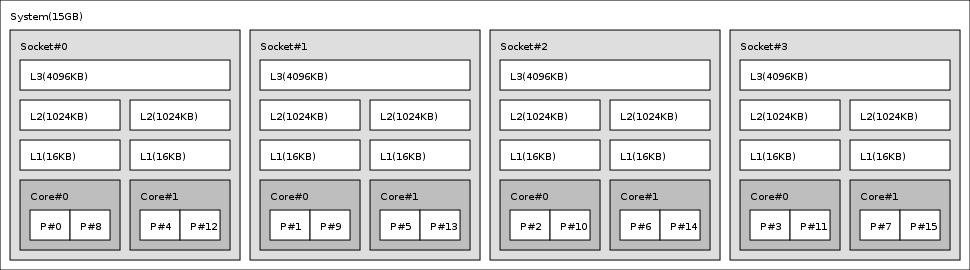
\includegraphics[width=\textwidth]{dudley.png}}
\end{ImageNoCaption}




\begin{Code}\begin{verbatim}System(15GB)
  Socket#0 + L3(4096KB)
    L2(1024KB) + L1(16KB) + Core#0
      P#0
      P#8
    L2(1024KB) + L1(16KB) + Core#1
      P#4
      P#12
  Socket#1 + L3(4096KB)
    L2(1024KB) + L1(16KB) + Core#0
      P#1
      P#9
    L2(1024KB) + L1(16KB) + Core#1
      P#5
      P#13
  Socket#2 + L3(4096KB)
    L2(1024KB) + L1(16KB) + Core#0
      P#2
      P#10
    L2(1024KB) + L1(16KB) + Core#1
      P#6
      P#14
  Socket#3 + L3(4096KB)
    L2(1024KB) + L1(16KB) + Core#0
      P#3
      P#11
    L2(1024KB) + L1(16KB) + Core#1
      P#7
      P#15
\end{verbatim}
\end{Code}



On a 4-socket 2-core Opteron NUMA machine, the {\tt lstopo} tool may show the following outputs:

 \begin{ImageNoCaption}\mbox{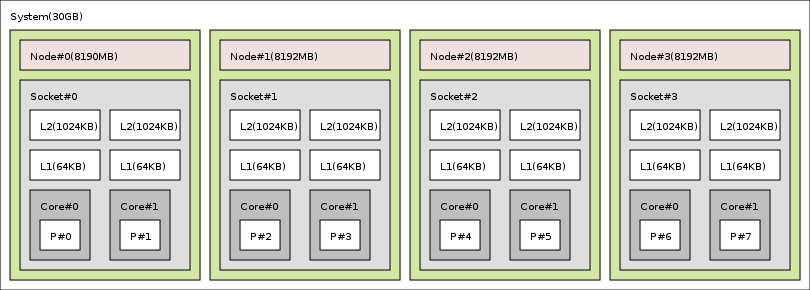
\includegraphics[width=\textwidth]{hagrid.png}}
\end{ImageNoCaption}




\begin{Code}\begin{verbatim}System(62GB)
  Node#0(8190MB) + Socket#0
    L2(1024KB) + L1(64KB) + Core#0 + P#0
    L2(1024KB) + L1(64KB) + Core#1 + P#1
  Node#1(8192MB) + Socket#1
    L2(1024KB) + L1(64KB) + Core#0 + P#2
    L2(1024KB) + L1(64KB) + Core#1 + P#3
  Node#2(8192MB) + Socket#2
    L2(1024KB) + L1(64KB) + Core#0 + P#4
    L2(1024KB) + L1(64KB) + Core#1 + P#5
  Node#3(8192MB) + Socket#3
    L2(1024KB) + L1(64KB) + Core#0 + P#6
    L2(1024KB) + L1(64KB) + Core#1 + P#7
  Node#4(8192MB) + Socket#4
    L2(1024KB) + L1(64KB) + Core#0 + P#8
    L2(1024KB) + L1(64KB) + Core#1 + P#9
  Node#5(8192MB) + Socket#5
    L2(1024KB) + L1(64KB) + Core#0 + P#10
    L2(1024KB) + L1(64KB) + Core#1 + P#11
  Node#6(8192MB) + Socket#6
    L2(1024KB) + L1(64KB) + Core#0 + P#12
    L2(1024KB) + L1(64KB) + Core#1 + P#13
  Node#7(8192MB) + Socket#7
    L2(1024KB) + L1(64KB) + Core#0 + P#14
    L2(1024KB) + L1(64KB) + Core#1 + P#15
\end{verbatim}
\end{Code}



On a 2-socket quad-core Xeon (pre-Nehalem ones assembling 2 dual-core dies into each socket):

 \begin{ImageNoCaption}\mbox{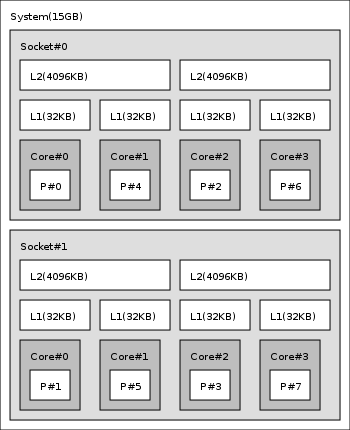
\includegraphics[width=\textwidth]{emmett.png}}
\end{ImageNoCaption}




\begin{Code}\begin{verbatim}System(15GB)
  Socket#0
    L2(4096KB)
      L1(32KB) + Core#0 + P#0
      L1(32KB) + Core#1 + P#4
    L2(4096KB)
      L1(32KB) + Core#2 + P#2
      L1(32KB) + Core#3 + P#6
  Socket#1
    L2(4096KB)
      L1(32KB) + Core#0 + P#1
      L1(32KB) + Core#1 + P#5
    L2(4096KB)
      L1(32KB) + Core#2 + P#3
      L1(32KB) + Core#3 + P#7
\end{verbatim}
\end{Code}



\hypertarget{index_interface}{}\section{Programming interface}\label{index_interface}
The basic interface is available in \hyperlink{hwloc_8h_source}{hwloc.h} . It mostly offers low-level routines for advanced programmers that want to manually manipulate objects and follow links between them. Most users should look at \hyperlink{helper_8h_source}{hwloc/helper.h} which provides a lot of interesting higher-level traversal examples.

Each object contains a cpuset which describes the list of processors that it contains. These cpusets may be used for \hyperlink{group__hwlocality__binding}{Binding}. hwloc offers an extensive cpuset manipulation interface in \hyperlink{cpuset_8h_source}{hwloc/cpuset.h} .

Moreover, hwloc also comes with additional helpers for interoperability with several commonly used environments. For Linux, some specific helpers are available in hwloc/linux.h , and \hyperlink{linux-libnuma_8h_source}{hwloc/linux-libnuma.h} if using libnuma. On glibc-based systems, additional helpers are available in \hyperlink{glibc-sched_8h_source}{hwloc/glibc-sched.h} . For systems with the Infiniband Verbs library, some dedicated helpers are provided in hwloc/ibverbs.h .

To precisely define the vocabulary used by hwloc, a \hyperlink{glossary}{Glossary} is available and should probably be read first.

Further documentation is available in html, manual pages, and pdf format in the source tarball in doc/doxygen-doc/ (after doxygen compilation for svn checkouts) and are installed in \$prefix/share/doc/hwloc/ and the usual manual repository.

The following section presents an example of API usage.\hypertarget{index_interface_example}{}\section{Interface example}\label{index_interface_example}
This section shows how to use hwloc with an small example {\tt hwloc-hello.c} that just prints the topology and binds itself to the first processor of the second core of the machine.

Hardware Location provides a pkg-config object, so compiling the example boils down to



\begin{footnotesize}\begin{verbatim}
CFLAGS+=$(pkg-config --cflags hwloc)
LDLIBS+=$(pkg-config --libs hwloc)
cc hwloc-hello.c $(CFLAGS) -o hwloc-hello $(LDLIBS)
\end{verbatim}
\end{footnotesize}




\begin{DocInclude}\begin{verbatim}/* topo-hello.c */
#include <hwloc.h>

static void print_children(hwloc_topology_t topology, hwloc_obj_t obj, int depth)
      
{
        char string[128];
        int i;

        hwloc_obj_snprintf(string, sizeof(string), topology, obj, "#", 0);
        printf("%*s%s\n", 2*depth, "", string);
        for (i = 0; i < obj->arity; i++)
                print_children(topology, obj->children[i], depth + 1);
}

int main(void)
{
        /* Topology object */
        hwloc_topology_t topology;

        /* Allocate and initialize topology object.  */
        hwloc_topology_init(&topology);

        /* ... Optionally, put detection configuration here to e.g. ignore some
           objects types, define a synthetic topology, etc....  The default is
           to detect all the objects of the machine that the caller is allowed
           to access.
           See Configure Topology Detection.  */

        /* Perform the topology detection.  */
        hwloc_topology_load(topology);


        /* Optionally, get some additional topology information
         * in case we need the topology depth later.
         */
        unsigned topodepth = hwloc_topology_get_depth(topology);


        /* Walk the topology with an array style, from level 0 (always the
         * system level) to the lowest level (always the proc level). */
        int depth, i;
        char string[128];
        for (depth = 0; depth < topodepth; depth++) {
                for (i = 0; i < hwloc_get_nbobjs_by_depth(topology, depth); i++) 
      {
                        hwloc_obj_snprintf(string, sizeof(string), topology,
                                        hwloc_get_obj_by_depth(topology, depth, i
      ), "#", 0);
                        printf("%s\n", string);
                }
        }

        /* Walk the topology with a tree style.  */
        print_children(topology, hwloc_get_system_obj(topology), 0);


        /* Print the number of sockets.  */
        depth = hwloc_get_type_depth(topology, HWLOC_OBJ_SOCKET);
        if (depth == HWLOC_TYPE_DEPTH_UNKNOWN)
                printf("The number of sockets is unknown\n");
        else
                printf("%u socket(s)\n", hwloc_get_nbobjs_by_depth(topology, dept
      h));


        /* Find out where cores are, or else smaller sets of CPUs if the OS
         * doesn't have the notion of core. */
        depth = hwloc_get_type_or_below_depth(topology, HWLOC_OBJ_CORE);

        /* Get last one.  */
        hwloc_obj_t obj = hwloc_get_obj_by_depth(topology, depth, 
      hwloc_get_nbobjs_by_depth(topology, depth) - 1);
        if (!obj)
                return 0;

        /* Get a copy of its cpuset that we may modify.  */
        hwloc_cpuset_t cpuset = hwloc_cpuset_dup(obj->cpuset);

        /* Get only one logical processor (in case the core is SMT/hyperthreaded)
      .  */
        hwloc_cpuset_singlify(cpuset);

        /* And try to bind ourself there.  */
        if (hwloc_set_cpubind(topology, cpuset, 0)) {
                char *str = NULL;
                hwloc_cpuset_asprintf(&str, obj->cpuset);
                printf("Couldn't bind to cpuset %s\n", str);
                free(str);
        }

        /* Free our cpuset copy */
        hwloc_cpuset_free(cpuset);

        /* Destroy topology object.  */
        hwloc_topology_destroy(topology);

        return 0;
}
\end{verbatim}
\end{DocInclude}


 \hypertarget{index_bugs}{}\section{Questions and bugs}\label{index_bugs}
Questions should be sent to the devel mailing list (\href{http://www.open-mpi.org/community/lists/hwloc.php}{\tt http://www.open-mpi.org/community/lists/hwloc.php}). Bug reports should be reported in the tracker (\href{https://svn.open-mpi.org/trac/hwloc/}{\tt https://svn.open-mpi.org/trac/hwloc/}).

 \hypertarget{index_history}{}\section{History / credits}\label{index_history}
hwloc is the evolution and merger of the libtopology (\href{http://runtime.bordeaux.inria.fr/libtopology/}{\tt http://runtime.bordeaux.inria.fr/libtopology/}) project and the Portable Linux Processor Affinity (PLPA) (\href{http://www.open-mpi.org/projects/plpa/}{\tt http://www.open-mpi.org/projects/plpa/}) project. Because of functional and ideological overlap, these two code bases and ideas were merged and released under the name \char`\"{}hwloc\char`\"{} as an Open MPI sub-project.

libtopology was initially developed by the INRIA Runtime Team-Project (\href{http://runtime.bordeaux.inria.fr/}{\tt http://runtime.bordeaux.inria.fr/}) (headed by Raymond Namyst (\href{http://dept-info.labri.fr/~namyst/}{\tt http://dept-info.labri.fr/$\sim$namyst/})). PLPA was initially developed by the Open MPI development team as a sub-project. Both are now deprecated in favor of hwloc, which is distributed as an Open MPI sub-project.

 

\chapter{Glossary}
\label{glossary}
\hypertarget{glossary}{}
\begin{description}
\item[Object ]Interesting kind of part of the system, such as a Core, a Cache, a Memory node, etc. The different types detected by hwloc are detailed in the hwloc\_\-obj\_\-type\_\-e enumeration.

They are topologically sorted by CPU set into a tree whose root is the System object which always exists. 

\item[CPU set ]The set of logical processors logically included in an object, if any

\item[Father object ]The object logically containing the current object, for instance because its CPU set includes the CPU set of the current object. 

\item[Children objects ]The object contained in the current object because their CPU set is included in the CPU set of the current object.

\item[Arity ]The number of children of an object

\item[Sibling objects ]Objects of the same type which have the same father

\item[Sibling rank ]Index to uniquely identify objecst of the same type which have the same father, numbered from 0 to the arity of the father minus one.

\item[Cousin objects ]Objects of the same type as the current object

\item[Level ]Set of objects of the same type

\item[OS index ]The index that the OS uses to identify the object. This may sometimes be completely arbitrary or depend on the BIOS configuration.

\item[Depth ]Nesting level in the object tree, starting from the System object.

\item[Logical index ]Index to uniquely identify objects of the same type. This index is always linear from 0 to the number of objects of the level for that type, to express proximity. It could also be called cousin rank.

\end{description}


The following diagram can help to understand the vocabulary of the relationships by showing the example of a machine with two dual core non-SMT sockets, thus a topology with 4 levels.

 \begin{ImageNoCaption}\mbox{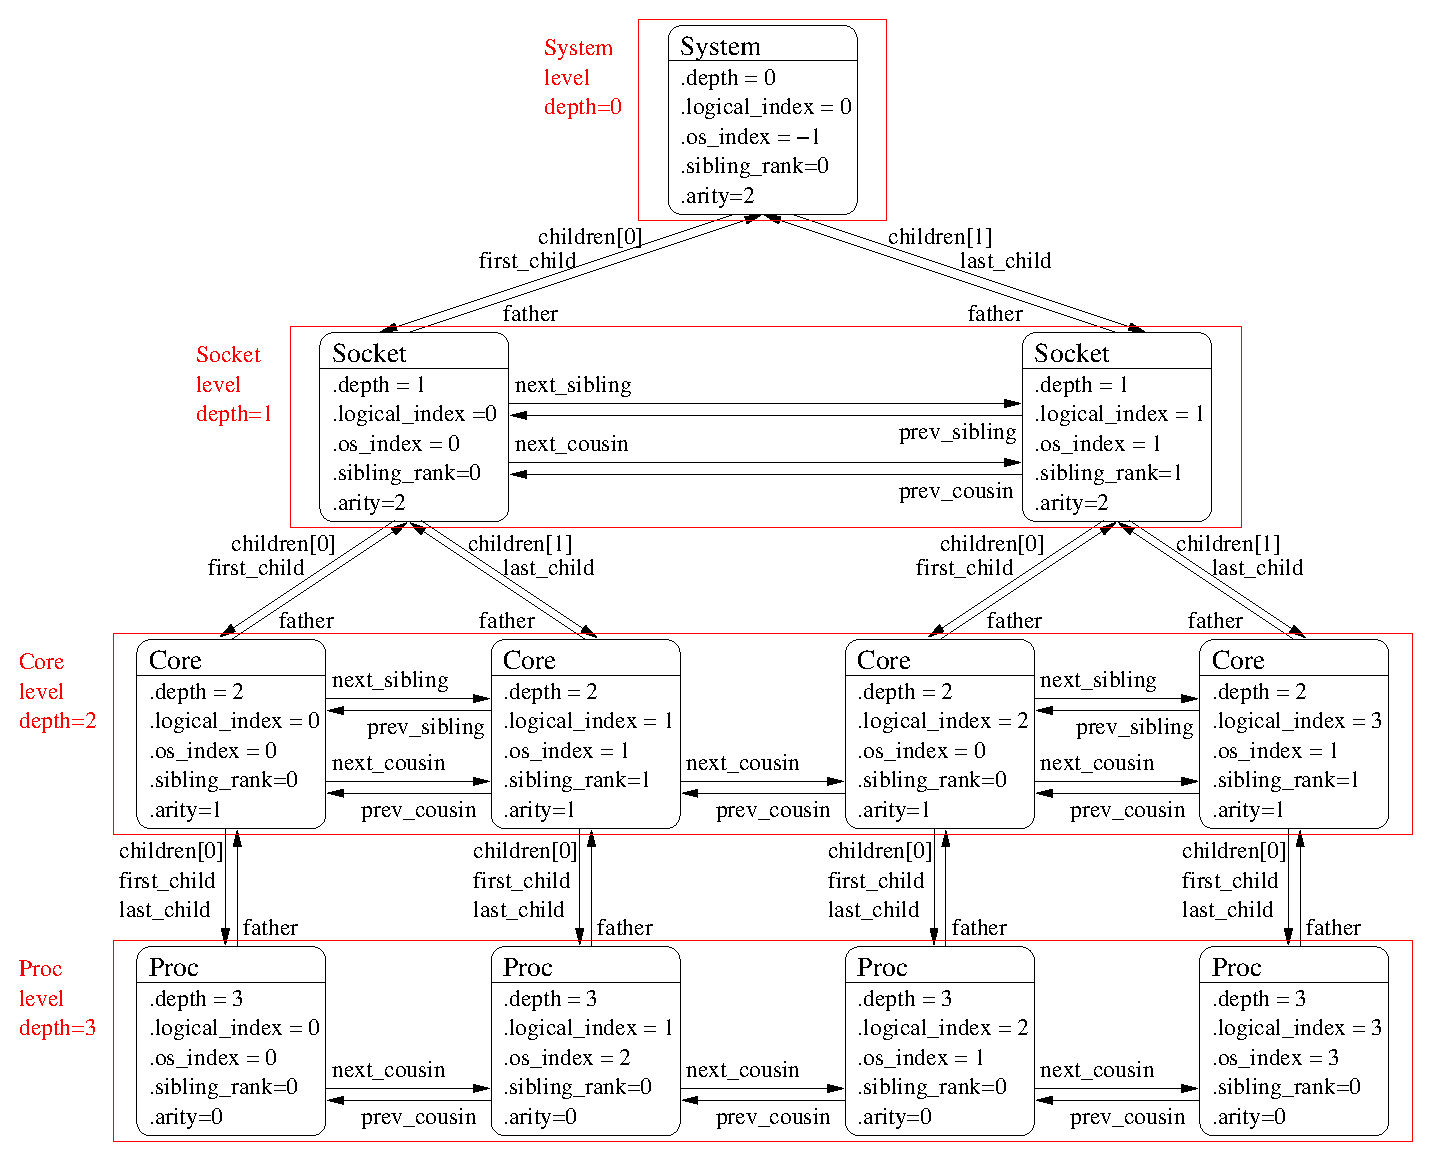
\includegraphics[width=\textwidth]{diagram}}
\end{ImageNoCaption}


It can be noticed that for Processor objects, the logical index, computed linearly by hwloc, is not the same as the OS index. 

\chapter{Module Index}
\section{Modules}
Here is a list of all modules:\begin{CompactList}
\item \contentsline{section}{Topology context}{\pageref{group__hwlocality__topology}}{}
\item \contentsline{section}{Topology Object Types}{\pageref{group__hwlocality__types}}{}
\item \contentsline{section}{Topology Objects}{\pageref{group__hwlocality__objects}}{}
\item \contentsline{section}{Create and Destroy Topologies}{\pageref{group__hwlocality__creation}}{}
\item \contentsline{section}{Configure Topology Detection}{\pageref{group__hwlocality__configuration}}{}
\item \contentsline{section}{Get some Topology Information}{\pageref{group__hwlocality__information}}{}
\item \contentsline{section}{Retrieve Objects}{\pageref{group__hwlocality__traversal}}{}
\item \contentsline{section}{Object/String Conversion}{\pageref{group__hwlocality__conversion}}{}
\item \contentsline{section}{Binding}{\pageref{group__hwlocality__binding}}{}
\item \contentsline{section}{Object Type Helpers}{\pageref{group__hwlocality__helper__types}}{}
\item \contentsline{section}{Basic Traversal Helpers}{\pageref{group__hwlocality__helper__traversal__basic}}{}
\item \contentsline{section}{Finding Objects Inside a CPU set}{\pageref{group__hwlocality__helper__find__inside}}{}
\item \contentsline{section}{Finding a single Object covering at least CPU set}{\pageref{group__hwlocality__helper__find__covering}}{}
\item \contentsline{section}{Finding a set of similar Objects covering at least a CPU set}{\pageref{group__hwlocality__helper__find__coverings}}{}
\item \contentsline{section}{Cache-specific Finding Helpers}{\pageref{group__hwlocality__helper__find__cache}}{}
\item \contentsline{section}{Advanced Traversal Helpers}{\pageref{group__hwlocality__helper__traversal}}{}
\item \contentsline{section}{Binding Helpers}{\pageref{group__hwlocality__helper__binding}}{}
\item \contentsline{section}{The Cpuset API}{\pageref{group__hwlocality__cpuset}}{}
\item \contentsline{section}{Helpers for manipulating glibc sched affinity}{\pageref{group__hwlocality__glibc__sched}}{}
\item \contentsline{section}{Helpers for manipulating Linux libnuma unsigned long masks}{\pageref{group__hwlocality__linux__libnuma__ulongs}}{}
\item \contentsline{section}{Helpers for manipulating Linux libnuma bitmask}{\pageref{group__hwlocality__linux__libnuma__bitmask}}{}
\item \contentsline{section}{Helpers for manipulating Linux libnuma nodemask\_\-t}{\pageref{group__hwlocality__linux__libnuma__nodemask}}{}
\end{CompactList}

\chapter{Data Structure Index}
\section{Data Structures}
Here are the data structures with brief descriptions:\begin{CompactList}
\item\contentsline{section}{\hyperlink{structhwloc__obj__attr__u_1_1hwloc__cache__attr__s}{hwloc\_\-obj\_\-attr\_\-u::hwloc\_\-cache\_\-attr\_\-s} (Cache-specific Object Attributes )}{\pageref{structhwloc__obj__attr__u_1_1hwloc__cache__attr__s}}{}
\item\contentsline{section}{\hyperlink{structhwloc__obj__attr__u_1_1hwloc__machine__attr__s}{hwloc\_\-obj\_\-attr\_\-u::hwloc\_\-machine\_\-attr\_\-s} (Machine-specific Object Attributes )}{\pageref{structhwloc__obj__attr__u_1_1hwloc__machine__attr__s}}{}
\item\contentsline{section}{\hyperlink{structhwloc__obj__attr__u_1_1hwloc__memory__attr__s}{hwloc\_\-obj\_\-attr\_\-u::hwloc\_\-memory\_\-attr\_\-s} (Node-specific Object Attributes )}{\pageref{structhwloc__obj__attr__u_1_1hwloc__memory__attr__s}}{}
\item\contentsline{section}{\hyperlink{structhwloc__obj__attr__u_1_1hwloc__misc__attr__s}{hwloc\_\-obj\_\-attr\_\-u::hwloc\_\-misc\_\-attr\_\-s} (Misc-specific Object Attributes )}{\pageref{structhwloc__obj__attr__u_1_1hwloc__misc__attr__s}}{}
\item\contentsline{section}{\hyperlink{structhwloc__obj}{hwloc\_\-obj} (Structure of a topology object )}{\pageref{structhwloc__obj}}{}
\item\contentsline{section}{\hyperlink{unionhwloc__obj__attr__u}{hwloc\_\-obj\_\-attr\_\-u} (Object type-specific Attributes )}{\pageref{unionhwloc__obj__attr__u}}{}
\end{CompactList}

\chapter{Module Documentation}
\hypertarget{group__hwlocality__topology}{
\section{Topology context}
\label{group__hwlocality__topology}\index{Topology context@{Topology context}}
}
\subsection*{Typedefs}
\begin{CompactItemize}
\item 
typedef struct hwloc\_\-topology $\ast$ \hyperlink{group__hwlocality__topology_g9d1e76ee15a7dee158b786c30b6a6e38}{hwloc\_\-topology\_\-t}
\begin{CompactList}\small\item\em Topology context. \item\end{CompactList}\end{CompactItemize}


\subsection{Typedef Documentation}
\hypertarget{group__hwlocality__topology_g9d1e76ee15a7dee158b786c30b6a6e38}{
\index{hwlocality\_\-topology@{hwlocality\_\-topology}!hwloc\_\-topology\_\-t@{hwloc\_\-topology\_\-t}}
\index{hwloc\_\-topology\_\-t@{hwloc\_\-topology\_\-t}!hwlocality_topology@{hwlocality\_\-topology}}
\subsubsection[{hwloc\_\-topology\_\-t}]{\setlength{\rightskip}{0pt plus 5cm}typedef struct hwloc\_\-topology$\ast$ {\bf hwloc\_\-topology\_\-t}}}
\label{group__hwlocality__topology_g9d1e76ee15a7dee158b786c30b6a6e38}


Topology context. 

To be initialized with \hyperlink{group__hwlocality__creation_g03fd4a16d8b9ee1ffc32b25fd2f6bdfa}{hwloc\_\-topology\_\-init()} and built with \hyperlink{group__hwlocality__creation_gbdf58d87ad77f6615fccdfe0535ff826}{hwloc\_\-topology\_\-load()}. 

\hypertarget{group__hwlocality__types}{
\section{Topology Object Types}
\label{group__hwlocality__types}\index{Topology Object Types@{Topology Object Types}}
}
\subsection*{Defines}
\begin{CompactItemize}
\item 
\#define \hyperlink{group__hwlocality__types_g3b6e4128e9fe773863b123fa6e4a080b}{HWLOC\_\-TYPE\_\-UNORDERED}~INT\_\-MAX
\begin{CompactList}\small\item\em Value returned by hwloc\_\-compare\_\-types when types can not be compared. \item\end{CompactList}\end{CompactItemize}
\subsection*{Enumerations}
\begin{CompactItemize}
\item 
enum \hyperlink{group__hwlocality__types_gcd37bb612667dc437d66bfb175a8dc55}{hwloc\_\-obj\_\-type\_\-t} \{ \par
\hyperlink{group__hwlocality__types_ggcd37bb612667dc437d66bfb175a8dc553aa1b842d1fd4207ebce171f95a244ec}{HWLOC\_\-OBJ\_\-SYSTEM}, 
\hyperlink{group__hwlocality__types_ggcd37bb612667dc437d66bfb175a8dc553f4e83ffc4a259354959ae8a9eaa2a80}{HWLOC\_\-OBJ\_\-MACHINE}, 
\hyperlink{group__hwlocality__types_ggcd37bb612667dc437d66bfb175a8dc55af0964881117bdedf1a5e9332cd120dd}{HWLOC\_\-OBJ\_\-NODE}, 
\hyperlink{group__hwlocality__types_ggcd37bb612667dc437d66bfb175a8dc551ac6e07775ae4324b3fe9dbd72c785ec}{HWLOC\_\-OBJ\_\-SOCKET}, 
\par
\hyperlink{group__hwlocality__types_ggcd37bb612667dc437d66bfb175a8dc5556ee0b7eca88f363b75b34fdde8c9ddc}{HWLOC\_\-OBJ\_\-CACHE}, 
\hyperlink{group__hwlocality__types_ggcd37bb612667dc437d66bfb175a8dc55c793958f330bca371aa1535de8aff45f}{HWLOC\_\-OBJ\_\-CORE}, 
\hyperlink{group__hwlocality__types_ggcd37bb612667dc437d66bfb175a8dc555e0ccbbd5922cbb07b53fe892b91b8f2}{HWLOC\_\-OBJ\_\-PROC}, 
\hyperlink{group__hwlocality__types_ggcd37bb612667dc437d66bfb175a8dc5519f8a6953fa91efc76bcbcdf2d22de4d}{HWLOC\_\-OBJ\_\-MISC}
 \}
\begin{CompactList}\small\item\em Type of topology object. \item\end{CompactList}\end{CompactItemize}
\subsection*{Functions}
\begin{CompactItemize}
\item 
int \hyperlink{group__hwlocality__types_g1820ea0dfd8e9dca28f9ea7624df5ae2}{hwloc\_\-compare\_\-types} (\hyperlink{group__hwlocality__types_gcd37bb612667dc437d66bfb175a8dc55}{hwloc\_\-obj\_\-type\_\-t} type1, \hyperlink{group__hwlocality__types_gcd37bb612667dc437d66bfb175a8dc55}{hwloc\_\-obj\_\-type\_\-t} type2)
\begin{CompactList}\small\item\em Compare the depth of two object types. \item\end{CompactList}\end{CompactItemize}


\subsection{Define Documentation}
\hypertarget{group__hwlocality__types_g3b6e4128e9fe773863b123fa6e4a080b}{
\index{hwlocality\_\-types@{hwlocality\_\-types}!HWLOC\_\-TYPE\_\-UNORDERED@{HWLOC\_\-TYPE\_\-UNORDERED}}
\index{HWLOC\_\-TYPE\_\-UNORDERED@{HWLOC\_\-TYPE\_\-UNORDERED}!hwlocality_types@{hwlocality\_\-types}}
\subsubsection[{HWLOC\_\-TYPE\_\-UNORDERED}]{\setlength{\rightskip}{0pt plus 5cm}\#define HWLOC\_\-TYPE\_\-UNORDERED~INT\_\-MAX}}
\label{group__hwlocality__types_g3b6e4128e9fe773863b123fa6e4a080b}


Value returned by hwloc\_\-compare\_\-types when types can not be compared. 



\subsection{Enumeration Type Documentation}
\hypertarget{group__hwlocality__types_gcd37bb612667dc437d66bfb175a8dc55}{
\index{hwlocality\_\-types@{hwlocality\_\-types}!hwloc\_\-obj\_\-type\_\-t@{hwloc\_\-obj\_\-type\_\-t}}
\index{hwloc\_\-obj\_\-type\_\-t@{hwloc\_\-obj\_\-type\_\-t}!hwlocality_types@{hwlocality\_\-types}}
\subsubsection[{hwloc\_\-obj\_\-type\_\-t}]{\setlength{\rightskip}{0pt plus 5cm}enum {\bf hwloc\_\-obj\_\-type\_\-t}}}
\label{group__hwlocality__types_gcd37bb612667dc437d66bfb175a8dc55}


Type of topology object. 

\begin{Desc}
\item[Note:]Do not rely on the ordering or completeness of the values as new ones may be defined in the future! If you need to compare types, use \hyperlink{group__hwlocality__types_g1820ea0dfd8e9dca28f9ea7624df5ae2}{hwloc\_\-compare\_\-types()} instead. \end{Desc}
\begin{Desc}
\item[Enumerator: ]\par
\begin{description}
\index{HWLOC\_\-OBJ\_\-SYSTEM@{HWLOC\_\-OBJ\_\-SYSTEM}!hwlocality\_\-types@{hwlocality\_\-types}}\index{hwlocality\_\-types@{hwlocality\_\-types}!HWLOC\_\-OBJ\_\-SYSTEM@{HWLOC\_\-OBJ\_\-SYSTEM}}\item[{\em 
\hypertarget{group__hwlocality__types_ggcd37bb612667dc437d66bfb175a8dc553aa1b842d1fd4207ebce171f95a244ec}{
HWLOC\_\-OBJ\_\-SYSTEM}
\label{group__hwlocality__types_ggcd37bb612667dc437d66bfb175a8dc553aa1b842d1fd4207ebce171f95a244ec}
}]Whole system (may be a cluster of machines). The whole system that is accessible to hwloc. That may comprise several machines in SSI systems like Kerrighed. \index{HWLOC\_\-OBJ\_\-MACHINE@{HWLOC\_\-OBJ\_\-MACHINE}!hwlocality\_\-types@{hwlocality\_\-types}}\index{hwlocality\_\-types@{hwlocality\_\-types}!HWLOC\_\-OBJ\_\-MACHINE@{HWLOC\_\-OBJ\_\-MACHINE}}\item[{\em 
\hypertarget{group__hwlocality__types_ggcd37bb612667dc437d66bfb175a8dc553f4e83ffc4a259354959ae8a9eaa2a80}{
HWLOC\_\-OBJ\_\-MACHINE}
\label{group__hwlocality__types_ggcd37bb612667dc437d66bfb175a8dc553f4e83ffc4a259354959ae8a9eaa2a80}
}]Machine. A set of processors and memory with cache coherency. \index{HWLOC\_\-OBJ\_\-NODE@{HWLOC\_\-OBJ\_\-NODE}!hwlocality\_\-types@{hwlocality\_\-types}}\index{hwlocality\_\-types@{hwlocality\_\-types}!HWLOC\_\-OBJ\_\-NODE@{HWLOC\_\-OBJ\_\-NODE}}\item[{\em 
\hypertarget{group__hwlocality__types_ggcd37bb612667dc437d66bfb175a8dc55af0964881117bdedf1a5e9332cd120dd}{
HWLOC\_\-OBJ\_\-NODE}
\label{group__hwlocality__types_ggcd37bb612667dc437d66bfb175a8dc55af0964881117bdedf1a5e9332cd120dd}
}]NUMA node. A set of processors around memory which the processors can directly access. \index{HWLOC\_\-OBJ\_\-SOCKET@{HWLOC\_\-OBJ\_\-SOCKET}!hwlocality\_\-types@{hwlocality\_\-types}}\index{hwlocality\_\-types@{hwlocality\_\-types}!HWLOC\_\-OBJ\_\-SOCKET@{HWLOC\_\-OBJ\_\-SOCKET}}\item[{\em 
\hypertarget{group__hwlocality__types_ggcd37bb612667dc437d66bfb175a8dc551ac6e07775ae4324b3fe9dbd72c785ec}{
HWLOC\_\-OBJ\_\-SOCKET}
\label{group__hwlocality__types_ggcd37bb612667dc437d66bfb175a8dc551ac6e07775ae4324b3fe9dbd72c785ec}
}]Socket, physical package, or chip. In the physical meaning, i.e. that you can add or remove physically. \index{HWLOC\_\-OBJ\_\-CACHE@{HWLOC\_\-OBJ\_\-CACHE}!hwlocality\_\-types@{hwlocality\_\-types}}\index{hwlocality\_\-types@{hwlocality\_\-types}!HWLOC\_\-OBJ\_\-CACHE@{HWLOC\_\-OBJ\_\-CACHE}}\item[{\em 
\hypertarget{group__hwlocality__types_ggcd37bb612667dc437d66bfb175a8dc5556ee0b7eca88f363b75b34fdde8c9ddc}{
HWLOC\_\-OBJ\_\-CACHE}
\label{group__hwlocality__types_ggcd37bb612667dc437d66bfb175a8dc5556ee0b7eca88f363b75b34fdde8c9ddc}
}]Data cache. Can be L1, L2, L3, ... \index{HWLOC\_\-OBJ\_\-CORE@{HWLOC\_\-OBJ\_\-CORE}!hwlocality\_\-types@{hwlocality\_\-types}}\index{hwlocality\_\-types@{hwlocality\_\-types}!HWLOC\_\-OBJ\_\-CORE@{HWLOC\_\-OBJ\_\-CORE}}\item[{\em 
\hypertarget{group__hwlocality__types_ggcd37bb612667dc437d66bfb175a8dc55c793958f330bca371aa1535de8aff45f}{
HWLOC\_\-OBJ\_\-CORE}
\label{group__hwlocality__types_ggcd37bb612667dc437d66bfb175a8dc55c793958f330bca371aa1535de8aff45f}
}]Core. A computation unit (may be shared by several logical processors). \index{HWLOC\_\-OBJ\_\-PROC@{HWLOC\_\-OBJ\_\-PROC}!hwlocality\_\-types@{hwlocality\_\-types}}\index{hwlocality\_\-types@{hwlocality\_\-types}!HWLOC\_\-OBJ\_\-PROC@{HWLOC\_\-OBJ\_\-PROC}}\item[{\em 
\hypertarget{group__hwlocality__types_ggcd37bb612667dc437d66bfb175a8dc555e0ccbbd5922cbb07b53fe892b91b8f2}{
HWLOC\_\-OBJ\_\-PROC}
\label{group__hwlocality__types_ggcd37bb612667dc437d66bfb175a8dc555e0ccbbd5922cbb07b53fe892b91b8f2}
}](Logical) Processor. An execution unit (may share a core with some other logical processors, e.g. in the case of an SMT core). 

Objects of this kind are always reported and can thus be used as fallback when others are not. \index{HWLOC\_\-OBJ\_\-MISC@{HWLOC\_\-OBJ\_\-MISC}!hwlocality\_\-types@{hwlocality\_\-types}}\index{hwlocality\_\-types@{hwlocality\_\-types}!HWLOC\_\-OBJ\_\-MISC@{HWLOC\_\-OBJ\_\-MISC}}\item[{\em 
\hypertarget{group__hwlocality__types_ggcd37bb612667dc437d66bfb175a8dc5519f8a6953fa91efc76bcbcdf2d22de4d}{
HWLOC\_\-OBJ\_\-MISC}
\label{group__hwlocality__types_ggcd37bb612667dc437d66bfb175a8dc5519f8a6953fa91efc76bcbcdf2d22de4d}
}]Miscellaneous objects. Objects which do not fit in the above but are detected by hwloc and are useful to take into account for affinity. For instance, some OSes expose their arbitrary processors aggregation this way. \end{description}
\end{Desc}



\subsection{Function Documentation}
\hypertarget{group__hwlocality__types_g1820ea0dfd8e9dca28f9ea7624df5ae2}{
\index{hwlocality\_\-types@{hwlocality\_\-types}!hwloc\_\-compare\_\-types@{hwloc\_\-compare\_\-types}}
\index{hwloc\_\-compare\_\-types@{hwloc\_\-compare\_\-types}!hwlocality_types@{hwlocality\_\-types}}
\subsubsection[{hwloc\_\-compare\_\-types}]{\setlength{\rightskip}{0pt plus 5cm}int hwloc\_\-compare\_\-types ({\bf hwloc\_\-obj\_\-type\_\-t} {\em type1}, \/  {\bf hwloc\_\-obj\_\-type\_\-t} {\em type2})}}
\label{group__hwlocality__types_g1820ea0dfd8e9dca28f9ea7624df5ae2}


Compare the depth of two object types. 

Types shouldn't be compared as they are, since newer ones may be added in the future. This function returns less than, equal to, or greater than zero if {\tt type1} is considered to be respectively higher than, equal to, or deeper than {\tt type2} in the hierarchy. If the types can not be compared (because it does not make sense), HWLOC\_\-TYPE\_\-UNORDERED is returned. Object types containing CPUs can always be compared.

\begin{Desc}
\item[Note:]HWLOC\_\-OBJ\_\-SYSTEM will always be the highest, and HWLOC\_\-OBJ\_\-PROC will always be the deepest. \end{Desc}

\hypertarget{group__hwlocality__objects}{
\section{Topology Objects}
\label{group__hwlocality__objects}\index{Topology Objects@{Topology Objects}}
}
\subsection*{Data Structures}
\begin{CompactItemize}
\item 
struct \hyperlink{structhwloc__obj}{hwloc\_\-obj}
\begin{CompactList}\small\item\em Structure of a topology object. \item\end{CompactList}\item 
union \hyperlink{unionhwloc__obj__attr__u}{hwloc\_\-obj\_\-attr\_\-u}
\begin{CompactList}\small\item\em Object type-specific Attributes. \item\end{CompactList}\end{CompactItemize}
\subsection*{Typedefs}
\begin{CompactItemize}
\item 
typedef struct \hyperlink{structhwloc__obj}{hwloc\_\-obj} $\ast$ \hyperlink{group__hwlocality__objects_g79b8ab56877ef99ac59b833203391c7d}{hwloc\_\-obj\_\-t}
\end{CompactItemize}


\subsection{Typedef Documentation}
\hypertarget{group__hwlocality__objects_g79b8ab56877ef99ac59b833203391c7d}{
\index{hwlocality\_\-objects@{hwlocality\_\-objects}!hwloc\_\-obj\_\-t@{hwloc\_\-obj\_\-t}}
\index{hwloc\_\-obj\_\-t@{hwloc\_\-obj\_\-t}!hwlocality_objects@{hwlocality\_\-objects}}
\subsubsection[{hwloc\_\-obj\_\-t}]{\setlength{\rightskip}{0pt plus 5cm}typedef struct {\bf hwloc\_\-obj}$\ast$ {\bf hwloc\_\-obj\_\-t}}}
\label{group__hwlocality__objects_g79b8ab56877ef99ac59b833203391c7d}



\hypertarget{group__hwlocality__creation}{
\section{Create and Destroy Topologies}
\label{group__hwlocality__creation}\index{Create and Destroy Topologies@{Create and Destroy Topologies}}
}
\subsection*{Functions}
\begin{CompactItemize}
\item 
int \hyperlink{group__hwlocality__creation_g03fd4a16d8b9ee1ffc32b25fd2f6bdfa}{hwloc\_\-topology\_\-init} (\hyperlink{group__hwlocality__topology_g9d1e76ee15a7dee158b786c30b6a6e38}{hwloc\_\-topology\_\-t} $\ast$topologyp)
\begin{CompactList}\small\item\em Allocate a topology context. \item\end{CompactList}\item 
int \hyperlink{group__hwlocality__creation_gbdf58d87ad77f6615fccdfe0535ff826}{hwloc\_\-topology\_\-load} (\hyperlink{group__hwlocality__topology_g9d1e76ee15a7dee158b786c30b6a6e38}{hwloc\_\-topology\_\-t} topology)
\begin{CompactList}\small\item\em Build the actual topology. \item\end{CompactList}\item 
void \hyperlink{group__hwlocality__creation_g9f34a640b6fd28d23699d4d084667b15}{hwloc\_\-topology\_\-destroy} (\hyperlink{group__hwlocality__topology_g9d1e76ee15a7dee158b786c30b6a6e38}{hwloc\_\-topology\_\-t} topology)
\begin{CompactList}\small\item\em Terminate and free a topology context. \item\end{CompactList}\item 
void \hyperlink{group__hwlocality__creation_gf6746bc3a558ef1ac8348b4491d091b5}{hwloc\_\-topology\_\-check} (\hyperlink{group__hwlocality__topology_g9d1e76ee15a7dee158b786c30b6a6e38}{hwloc\_\-topology\_\-t} topology)
\begin{CompactList}\small\item\em Run internal checks on a topology structure. \item\end{CompactList}\end{CompactItemize}


\subsection{Function Documentation}
\hypertarget{group__hwlocality__creation_gf6746bc3a558ef1ac8348b4491d091b5}{
\index{hwlocality\_\-creation@{hwlocality\_\-creation}!hwloc\_\-topology\_\-check@{hwloc\_\-topology\_\-check}}
\index{hwloc\_\-topology\_\-check@{hwloc\_\-topology\_\-check}!hwlocality_creation@{hwlocality\_\-creation}}
\subsubsection[{hwloc\_\-topology\_\-check}]{\setlength{\rightskip}{0pt plus 5cm}void hwloc\_\-topology\_\-check ({\bf hwloc\_\-topology\_\-t} {\em topology})}}
\label{group__hwlocality__creation_gf6746bc3a558ef1ac8348b4491d091b5}


Run internal checks on a topology structure. 

\begin{Desc}
\item[Parameters:]
\begin{description}
\item[{\em topology}]is the topology to be checked \end{description}
\end{Desc}
\hypertarget{group__hwlocality__creation_g9f34a640b6fd28d23699d4d084667b15}{
\index{hwlocality\_\-creation@{hwlocality\_\-creation}!hwloc\_\-topology\_\-destroy@{hwloc\_\-topology\_\-destroy}}
\index{hwloc\_\-topology\_\-destroy@{hwloc\_\-topology\_\-destroy}!hwlocality_creation@{hwlocality\_\-creation}}
\subsubsection[{hwloc\_\-topology\_\-destroy}]{\setlength{\rightskip}{0pt plus 5cm}void hwloc\_\-topology\_\-destroy ({\bf hwloc\_\-topology\_\-t} {\em topology})}}
\label{group__hwlocality__creation_g9f34a640b6fd28d23699d4d084667b15}


Terminate and free a topology context. 

\begin{Desc}
\item[Parameters:]
\begin{description}
\item[{\em topology}]is the topology to be freed \end{description}
\end{Desc}
\hypertarget{group__hwlocality__creation_g03fd4a16d8b9ee1ffc32b25fd2f6bdfa}{
\index{hwlocality\_\-creation@{hwlocality\_\-creation}!hwloc\_\-topology\_\-init@{hwloc\_\-topology\_\-init}}
\index{hwloc\_\-topology\_\-init@{hwloc\_\-topology\_\-init}!hwlocality_creation@{hwlocality\_\-creation}}
\subsubsection[{hwloc\_\-topology\_\-init}]{\setlength{\rightskip}{0pt plus 5cm}int hwloc\_\-topology\_\-init ({\bf hwloc\_\-topology\_\-t} $\ast$ {\em topologyp})}}
\label{group__hwlocality__creation_g03fd4a16d8b9ee1ffc32b25fd2f6bdfa}


Allocate a topology context. 

\begin{Desc}
\item[Parameters:]
\begin{description}
\item[\mbox{$\rightarrow$} {\em topologyp}]is assigned a pointer to the new allocated context.\end{description}
\end{Desc}
\begin{Desc}
\item[Returns:]0 on success, -1 on error. \end{Desc}
\hypertarget{group__hwlocality__creation_gbdf58d87ad77f6615fccdfe0535ff826}{
\index{hwlocality\_\-creation@{hwlocality\_\-creation}!hwloc\_\-topology\_\-load@{hwloc\_\-topology\_\-load}}
\index{hwloc\_\-topology\_\-load@{hwloc\_\-topology\_\-load}!hwlocality_creation@{hwlocality\_\-creation}}
\subsubsection[{hwloc\_\-topology\_\-load}]{\setlength{\rightskip}{0pt plus 5cm}int hwloc\_\-topology\_\-load ({\bf hwloc\_\-topology\_\-t} {\em topology})}}
\label{group__hwlocality__creation_gbdf58d87ad77f6615fccdfe0535ff826}


Build the actual topology. 

Build the actual topology once initialized with \hyperlink{group__hwlocality__creation_g03fd4a16d8b9ee1ffc32b25fd2f6bdfa}{hwloc\_\-topology\_\-init()} and tuned with hwlocality\_\-configuration routine. No other routine may be called earlier using this topology context.

\begin{Desc}
\item[Parameters:]
\begin{description}
\item[{\em topology}]is the topology to be loaded with objects.\end{description}
\end{Desc}
\begin{Desc}
\item[Returns:]0 on success, -1 on error.\end{Desc}
\begin{Desc}
\item[See also:]\hyperlink{group__hwlocality__configuration}{Configure Topology Detection} \end{Desc}

\hypertarget{group__hwlocality__configuration}{
\section{Configure Topology Detection}
\label{group__hwlocality__configuration}\index{Configure Topology Detection@{Configure Topology Detection}}
}
\subsection*{Enumerations}
\begin{CompactItemize}
\item 
enum \hyperlink{group__hwlocality__configuration_gda025d3ec20b4b420f8038d23d6e7bde}{hwloc\_\-topology\_\-flags\_\-e} \{ \hyperlink{group__hwlocality__configuration_ggda025d3ec20b4b420f8038d23d6e7bde129b4fea1300be22bbaf0bb0958994c8}{HWLOC\_\-TOPOLOGY\_\-FLAG\_\-WHOLE\_\-SYSTEM} =  (1$<$$<$0), 
\hyperlink{group__hwlocality__configuration_ggda025d3ec20b4b420f8038d23d6e7bde6ecb6abc6a0bb75e81564f8bca85783b}{HWLOC\_\-TOPOLOGY\_\-FLAG\_\-IS\_\-THISSYSTEM} =  (1$<$$<$1)
 \}
\begin{CompactList}\small\item\em Flags to be set onto a topology context before load. \item\end{CompactList}\end{CompactItemize}
\subsection*{Functions}
\begin{CompactItemize}
\item 
int \hyperlink{group__hwlocality__configuration_gfcf30842e8cb47b4c3dcaebecea31e17}{hwloc\_\-topology\_\-ignore\_\-type} (\hyperlink{group__hwlocality__topology_g9d1e76ee15a7dee158b786c30b6a6e38}{hwloc\_\-topology\_\-t} topology, \hyperlink{group__hwlocality__types_gcd37bb612667dc437d66bfb175a8dc55}{hwloc\_\-obj\_\-type\_\-t} type)
\begin{CompactList}\small\item\em Ignore an object type. \item\end{CompactList}\item 
int \hyperlink{group__hwlocality__configuration_g1f987bca941d6949faf7b1554dd7bc12}{hwloc\_\-topology\_\-ignore\_\-type\_\-keep\_\-structure} (\hyperlink{group__hwlocality__topology_g9d1e76ee15a7dee158b786c30b6a6e38}{hwloc\_\-topology\_\-t} topology, \hyperlink{group__hwlocality__types_gcd37bb612667dc437d66bfb175a8dc55}{hwloc\_\-obj\_\-type\_\-t} type)
\begin{CompactList}\small\item\em Ignore an object type if it does not bring any structure. \item\end{CompactList}\item 
int \hyperlink{group__hwlocality__configuration_g7c9cf147442d65d755c664ccde3bb3ef}{hwloc\_\-topology\_\-ignore\_\-all\_\-keep\_\-structure} (\hyperlink{group__hwlocality__topology_g9d1e76ee15a7dee158b786c30b6a6e38}{hwloc\_\-topology\_\-t} topology)
\begin{CompactList}\small\item\em Ignore all objects that do not bring any structure. \item\end{CompactList}\item 
int \hyperlink{group__hwlocality__configuration_gaeed4df656979e5f16befea9d29b814b}{hwloc\_\-topology\_\-set\_\-flags} (\hyperlink{group__hwlocality__topology_g9d1e76ee15a7dee158b786c30b6a6e38}{hwloc\_\-topology\_\-t} topology, unsigned long flags)
\begin{CompactList}\small\item\em Set OR'ed flags to non-yet-loaded topology. \item\end{CompactList}\item 
int \hyperlink{group__hwlocality__configuration_g45a6b5dd59be36879a64a7f73e0363c2}{hwloc\_\-topology\_\-set\_\-fsroot} (\hyperlink{group__hwlocality__topology_g9d1e76ee15a7dee158b786c30b6a6e38}{hwloc\_\-topology\_\-t} restrict topology, const char $\ast$restrict fsroot\_\-path)
\begin{CompactList}\small\item\em Change the file-system root path when building the topology from sysfs/procfs. \item\end{CompactList}\item 
int \hyperlink{group__hwlocality__configuration_g5c11f6e454ebd5f4089670269e097a1e}{hwloc\_\-topology\_\-set\_\-synthetic} (\hyperlink{group__hwlocality__topology_g9d1e76ee15a7dee158b786c30b6a6e38}{hwloc\_\-topology\_\-t} restrict topology, const char $\ast$restrict description)
\begin{CompactList}\small\item\em Enable synthetic topology. \item\end{CompactList}\item 
int \hyperlink{group__hwlocality__configuration_g29b8ebec1b85b324af18fdf5040806bf}{hwloc\_\-topology\_\-set\_\-xml} (\hyperlink{group__hwlocality__topology_g9d1e76ee15a7dee158b786c30b6a6e38}{hwloc\_\-topology\_\-t} restrict topology, const char $\ast$restrict xmlpath)
\begin{CompactList}\small\item\em Enable XML-file based topology. \item\end{CompactList}\end{CompactItemize}


\subsection{Detailed Description}
These functions can optionally be called between \hyperlink{group__hwlocality__creation_g03fd4a16d8b9ee1ffc32b25fd2f6bdfa}{hwloc\_\-topology\_\-init()} and \hyperlink{group__hwlocality__creation_gbdf58d87ad77f6615fccdfe0535ff826}{hwloc\_\-topology\_\-load()} to configure how the detection should be performed, e.g. to ignore some objects types, define a synthetic topology, etc.

If none of them is called, the default is to detect all the objects of the machine that the caller is allowed to access. 

\subsection{Enumeration Type Documentation}
\hypertarget{group__hwlocality__configuration_gda025d3ec20b4b420f8038d23d6e7bde}{
\index{hwlocality\_\-configuration@{hwlocality\_\-configuration}!hwloc\_\-topology\_\-flags\_\-e@{hwloc\_\-topology\_\-flags\_\-e}}
\index{hwloc\_\-topology\_\-flags\_\-e@{hwloc\_\-topology\_\-flags\_\-e}!hwlocality_configuration@{hwlocality\_\-configuration}}
\subsubsection[{hwloc\_\-topology\_\-flags\_\-e}]{\setlength{\rightskip}{0pt plus 5cm}enum {\bf hwloc\_\-topology\_\-flags\_\-e}}}
\label{group__hwlocality__configuration_gda025d3ec20b4b420f8038d23d6e7bde}


Flags to be set onto a topology context before load. 

Flags should be given to \hyperlink{group__hwlocality__configuration_gaeed4df656979e5f16befea9d29b814b}{hwloc\_\-topology\_\-set\_\-flags()}. \begin{Desc}
\item[Enumerator: ]\par
\begin{description}
\index{HWLOC\_\-TOPOLOGY\_\-FLAG\_\-WHOLE\_\-SYSTEM@{HWLOC\_\-TOPOLOGY\_\-FLAG\_\-WHOLE\_\-SYSTEM}!hwlocality\_\-configuration@{hwlocality\_\-configuration}}\index{hwlocality\_\-configuration@{hwlocality\_\-configuration}!HWLOC\_\-TOPOLOGY\_\-FLAG\_\-WHOLE\_\-SYSTEM@{HWLOC\_\-TOPOLOGY\_\-FLAG\_\-WHOLE\_\-SYSTEM}}\item[{\em 
\hypertarget{group__hwlocality__configuration_ggda025d3ec20b4b420f8038d23d6e7bde129b4fea1300be22bbaf0bb0958994c8}{
HWLOC\_\-TOPOLOGY\_\-FLAG\_\-WHOLE\_\-SYSTEM}
\label{group__hwlocality__configuration_ggda025d3ec20b4b420f8038d23d6e7bde129b4fea1300be22bbaf0bb0958994c8}
}]\index{HWLOC\_\-TOPOLOGY\_\-FLAG\_\-IS\_\-THISSYSTEM@{HWLOC\_\-TOPOLOGY\_\-FLAG\_\-IS\_\-THISSYSTEM}!hwlocality\_\-configuration@{hwlocality\_\-configuration}}\index{hwlocality\_\-configuration@{hwlocality\_\-configuration}!HWLOC\_\-TOPOLOGY\_\-FLAG\_\-IS\_\-THISSYSTEM@{HWLOC\_\-TOPOLOGY\_\-FLAG\_\-IS\_\-THISSYSTEM}}\item[{\em 
\hypertarget{group__hwlocality__configuration_ggda025d3ec20b4b420f8038d23d6e7bde6ecb6abc6a0bb75e81564f8bca85783b}{
HWLOC\_\-TOPOLOGY\_\-FLAG\_\-IS\_\-THISSYSTEM}
\label{group__hwlocality__configuration_ggda025d3ec20b4b420f8038d23d6e7bde6ecb6abc6a0bb75e81564f8bca85783b}
}]\end{description}
\end{Desc}



\subsection{Function Documentation}
\hypertarget{group__hwlocality__configuration_g7c9cf147442d65d755c664ccde3bb3ef}{
\index{hwlocality\_\-configuration@{hwlocality\_\-configuration}!hwloc\_\-topology\_\-ignore\_\-all\_\-keep\_\-structure@{hwloc\_\-topology\_\-ignore\_\-all\_\-keep\_\-structure}}
\index{hwloc\_\-topology\_\-ignore\_\-all\_\-keep\_\-structure@{hwloc\_\-topology\_\-ignore\_\-all\_\-keep\_\-structure}!hwlocality_configuration@{hwlocality\_\-configuration}}
\subsubsection[{hwloc\_\-topology\_\-ignore\_\-all\_\-keep\_\-structure}]{\setlength{\rightskip}{0pt plus 5cm}int hwloc\_\-topology\_\-ignore\_\-all\_\-keep\_\-structure ({\bf hwloc\_\-topology\_\-t} {\em topology})}}
\label{group__hwlocality__configuration_g7c9cf147442d65d755c664ccde3bb3ef}


Ignore all objects that do not bring any structure. 

Ignore all objects that do not bring any structure: Each ignored object should have a single children or be the only child of its father. \hypertarget{group__hwlocality__configuration_gfcf30842e8cb47b4c3dcaebecea31e17}{
\index{hwlocality\_\-configuration@{hwlocality\_\-configuration}!hwloc\_\-topology\_\-ignore\_\-type@{hwloc\_\-topology\_\-ignore\_\-type}}
\index{hwloc\_\-topology\_\-ignore\_\-type@{hwloc\_\-topology\_\-ignore\_\-type}!hwlocality_configuration@{hwlocality\_\-configuration}}
\subsubsection[{hwloc\_\-topology\_\-ignore\_\-type}]{\setlength{\rightskip}{0pt plus 5cm}int hwloc\_\-topology\_\-ignore\_\-type ({\bf hwloc\_\-topology\_\-t} {\em topology}, \/  {\bf hwloc\_\-obj\_\-type\_\-t} {\em type})}}
\label{group__hwlocality__configuration_gfcf30842e8cb47b4c3dcaebecea31e17}


Ignore an object type. 

Ignore all objects from the given type. The top-level type HWLOC\_\-OBJ\_\-SYSTEM and bottom-level type HWLOC\_\-OBJ\_\-PROC may not be ignored. \hypertarget{group__hwlocality__configuration_g1f987bca941d6949faf7b1554dd7bc12}{
\index{hwlocality\_\-configuration@{hwlocality\_\-configuration}!hwloc\_\-topology\_\-ignore\_\-type\_\-keep\_\-structure@{hwloc\_\-topology\_\-ignore\_\-type\_\-keep\_\-structure}}
\index{hwloc\_\-topology\_\-ignore\_\-type\_\-keep\_\-structure@{hwloc\_\-topology\_\-ignore\_\-type\_\-keep\_\-structure}!hwlocality_configuration@{hwlocality\_\-configuration}}
\subsubsection[{hwloc\_\-topology\_\-ignore\_\-type\_\-keep\_\-structure}]{\setlength{\rightskip}{0pt plus 5cm}int hwloc\_\-topology\_\-ignore\_\-type\_\-keep\_\-structure ({\bf hwloc\_\-topology\_\-t} {\em topology}, \/  {\bf hwloc\_\-obj\_\-type\_\-t} {\em type})}}
\label{group__hwlocality__configuration_g1f987bca941d6949faf7b1554dd7bc12}


Ignore an object type if it does not bring any structure. 

Ignore all objects from the given type as long as they do not bring any structure: Each ignored object should have a single children or be the only child of its father. The top-level type HWLOC\_\-OBJ\_\-SYSTEM and bottom-level type HWLOC\_\-OBJ\_\-PROC may not be ignored. \hypertarget{group__hwlocality__configuration_gaeed4df656979e5f16befea9d29b814b}{
\index{hwlocality\_\-configuration@{hwlocality\_\-configuration}!hwloc\_\-topology\_\-set\_\-flags@{hwloc\_\-topology\_\-set\_\-flags}}
\index{hwloc\_\-topology\_\-set\_\-flags@{hwloc\_\-topology\_\-set\_\-flags}!hwlocality_configuration@{hwlocality\_\-configuration}}
\subsubsection[{hwloc\_\-topology\_\-set\_\-flags}]{\setlength{\rightskip}{0pt plus 5cm}int hwloc\_\-topology\_\-set\_\-flags ({\bf hwloc\_\-topology\_\-t} {\em topology}, \/  unsigned long {\em flags})}}
\label{group__hwlocality__configuration_gaeed4df656979e5f16befea9d29b814b}


Set OR'ed flags to non-yet-loaded topology. 

Set a OR'ed set of hwloc\_\-topology\_\-flags\_\-e onto a topology that was not yet loaded. \hypertarget{group__hwlocality__configuration_g45a6b5dd59be36879a64a7f73e0363c2}{
\index{hwlocality\_\-configuration@{hwlocality\_\-configuration}!hwloc\_\-topology\_\-set\_\-fsroot@{hwloc\_\-topology\_\-set\_\-fsroot}}
\index{hwloc\_\-topology\_\-set\_\-fsroot@{hwloc\_\-topology\_\-set\_\-fsroot}!hwlocality_configuration@{hwlocality\_\-configuration}}
\subsubsection[{hwloc\_\-topology\_\-set\_\-fsroot}]{\setlength{\rightskip}{0pt plus 5cm}int hwloc\_\-topology\_\-set\_\-fsroot ({\bf hwloc\_\-topology\_\-t} restrict {\em topology}, \/  const char $\ast$restrict {\em fsroot\_\-path})}}
\label{group__hwlocality__configuration_g45a6b5dd59be36879a64a7f73e0363c2}


Change the file-system root path when building the topology from sysfs/procfs. 

On Linux system, use sysfs and procfs files as if they were mounted on the given {\tt fsroot\_\-path} instead of the main file-system root. Not using the main file-system root causes hwloc\_\-topology\_\-is\_\-thissystem field to return 0.

\begin{Desc}
\item[Note:]For conveniency, this backend provides empty binding hooks which just return success. To have hwloc still actually call OS-specific hooks, the HWLOC\_\-TOPOLOGY\_\-FLAG\_\-IS\_\-THISSYSTEM has to be set to assert that the loaded file is really the underlying system. \end{Desc}
\hypertarget{group__hwlocality__configuration_g5c11f6e454ebd5f4089670269e097a1e}{
\index{hwlocality\_\-configuration@{hwlocality\_\-configuration}!hwloc\_\-topology\_\-set\_\-synthetic@{hwloc\_\-topology\_\-set\_\-synthetic}}
\index{hwloc\_\-topology\_\-set\_\-synthetic@{hwloc\_\-topology\_\-set\_\-synthetic}!hwlocality_configuration@{hwlocality\_\-configuration}}
\subsubsection[{hwloc\_\-topology\_\-set\_\-synthetic}]{\setlength{\rightskip}{0pt plus 5cm}int hwloc\_\-topology\_\-set\_\-synthetic ({\bf hwloc\_\-topology\_\-t} restrict {\em topology}, \/  const char $\ast$restrict {\em description})}}
\label{group__hwlocality__configuration_g5c11f6e454ebd5f4089670269e097a1e}


Enable synthetic topology. 

Gather topology information from the given {\tt description} which should be a comma separated string of numbers describing the arity of each level. Each number may be prefixed with a type and a colon to enforce the type of a level.

\begin{Desc}
\item[Note:]For conveniency, this backend provides empty binding hooks which just return success. \end{Desc}
\hypertarget{group__hwlocality__configuration_g29b8ebec1b85b324af18fdf5040806bf}{
\index{hwlocality\_\-configuration@{hwlocality\_\-configuration}!hwloc\_\-topology\_\-set\_\-xml@{hwloc\_\-topology\_\-set\_\-xml}}
\index{hwloc\_\-topology\_\-set\_\-xml@{hwloc\_\-topology\_\-set\_\-xml}!hwlocality_configuration@{hwlocality\_\-configuration}}
\subsubsection[{hwloc\_\-topology\_\-set\_\-xml}]{\setlength{\rightskip}{0pt plus 5cm}int hwloc\_\-topology\_\-set\_\-xml ({\bf hwloc\_\-topology\_\-t} restrict {\em topology}, \/  const char $\ast$restrict {\em xmlpath})}}
\label{group__hwlocality__configuration_g29b8ebec1b85b324af18fdf5040806bf}


Enable XML-file based topology. 

Gather topology information the XML file given at {\tt xmlpath}. This file may have been generated earlier with lstopo file.xml.

\begin{Desc}
\item[Note:]For conveniency, this backend provides empty binding hooks which just return success. To have hwloc still actually call OS-specific hooks, the HWLOC\_\-TOPOLOGY\_\-FLAG\_\-IS\_\-THISSYSTEM has to be set to assert that the loaded file is really the underlying system. \end{Desc}

\hypertarget{group__hwlocality__information}{
\section{Get some Topology Information}
\label{group__hwlocality__information}\index{Get some Topology Information@{Get some Topology Information}}
}
\subsection*{Defines}
\begin{CompactItemize}
\item 
\#define \hyperlink{group__hwlocality__information_g9e86ce528f626330de2da7adb6c4e02e}{HWLOC\_\-TYPE\_\-DEPTH\_\-UNKNOWN}~-1
\begin{CompactList}\small\item\em No object of given type exists in the topology. \item\end{CompactList}\item 
\#define \hyperlink{group__hwlocality__information_g64c80d3e0501b321d217b1642d68e23d}{HWLOC\_\-TYPE\_\-DEPTH\_\-MULTIPLE}~-2
\begin{CompactList}\small\item\em Objects of given type exist at different depth in the topology. \item\end{CompactList}\end{CompactItemize}
\subsection*{Functions}
\begin{CompactItemize}
\item 
unsigned \hyperlink{group__hwlocality__information_g3cc2255e237b751a6c8efa8703b3daf5}{hwloc\_\-topology\_\-get\_\-depth} (\hyperlink{group__hwlocality__topology_g9d1e76ee15a7dee158b786c30b6a6e38}{hwloc\_\-topology\_\-t} restrict topology)
\begin{CompactList}\small\item\em Get the depth of the hierachical tree of objects. \item\end{CompactList}\item 
int \hyperlink{group__hwlocality__information_g8bec782e21be313750da70cf7428b374}{hwloc\_\-get\_\-type\_\-depth} (\hyperlink{group__hwlocality__topology_g9d1e76ee15a7dee158b786c30b6a6e38}{hwloc\_\-topology\_\-t} topology, \hyperlink{group__hwlocality__types_gcd37bb612667dc437d66bfb175a8dc55}{hwloc\_\-obj\_\-type\_\-t} type)
\begin{CompactList}\small\item\em Returns the depth of objects of type {\tt type}. \item\end{CompactList}\item 
\hyperlink{group__hwlocality__types_gcd37bb612667dc437d66bfb175a8dc55}{hwloc\_\-obj\_\-type\_\-t} \hyperlink{group__hwlocality__information_g8cc04ad9eb03b0b74d420adf8cc11ad2}{hwloc\_\-get\_\-depth\_\-type} (\hyperlink{group__hwlocality__topology_g9d1e76ee15a7dee158b786c30b6a6e38}{hwloc\_\-topology\_\-t} topology, unsigned depth)
\begin{CompactList}\small\item\em Returns the type of objects at depth {\tt depth}. \item\end{CompactList}\item 
unsigned \hyperlink{group__hwlocality__information_gb17065e3d53455973844568d9f21c72c}{hwloc\_\-get\_\-nbobjs\_\-by\_\-depth} (\hyperlink{group__hwlocality__topology_g9d1e76ee15a7dee158b786c30b6a6e38}{hwloc\_\-topology\_\-t} topology, unsigned depth)
\begin{CompactList}\small\item\em Returns the width of level at depth {\tt depth}. \item\end{CompactList}\item 
static inline int \hyperlink{group__hwlocality__information_gd86a90c0d3501d90410fb1a4eb36f5d0}{hwloc\_\-get\_\-nbobjs\_\-by\_\-type} (\hyperlink{group__hwlocality__topology_g9d1e76ee15a7dee158b786c30b6a6e38}{hwloc\_\-topology\_\-t} topology, \hyperlink{group__hwlocality__types_gcd37bb612667dc437d66bfb175a8dc55}{hwloc\_\-obj\_\-type\_\-t} type)
\begin{CompactList}\small\item\em Returns the width of level type {\tt type}. \item\end{CompactList}\item 
int \hyperlink{group__hwlocality__information_g29cdfde981aafc92eb89639a36b1ff9b}{hwloc\_\-topology\_\-is\_\-thissystem} (\hyperlink{group__hwlocality__topology_g9d1e76ee15a7dee158b786c30b6a6e38}{hwloc\_\-topology\_\-t} restrict topology)
\begin{CompactList}\small\item\em Does the topology context come from this system? \item\end{CompactList}\end{CompactItemize}


\subsection{Define Documentation}
\hypertarget{group__hwlocality__information_g64c80d3e0501b321d217b1642d68e23d}{
\index{hwlocality\_\-information@{hwlocality\_\-information}!HWLOC\_\-TYPE\_\-DEPTH\_\-MULTIPLE@{HWLOC\_\-TYPE\_\-DEPTH\_\-MULTIPLE}}
\index{HWLOC\_\-TYPE\_\-DEPTH\_\-MULTIPLE@{HWLOC\_\-TYPE\_\-DEPTH\_\-MULTIPLE}!hwlocality_information@{hwlocality\_\-information}}
\subsubsection[{HWLOC\_\-TYPE\_\-DEPTH\_\-MULTIPLE}]{\setlength{\rightskip}{0pt plus 5cm}\#define HWLOC\_\-TYPE\_\-DEPTH\_\-MULTIPLE~-2}}
\label{group__hwlocality__information_g64c80d3e0501b321d217b1642d68e23d}


Objects of given type exist at different depth in the topology. 

\hypertarget{group__hwlocality__information_g9e86ce528f626330de2da7adb6c4e02e}{
\index{hwlocality\_\-information@{hwlocality\_\-information}!HWLOC\_\-TYPE\_\-DEPTH\_\-UNKNOWN@{HWLOC\_\-TYPE\_\-DEPTH\_\-UNKNOWN}}
\index{HWLOC\_\-TYPE\_\-DEPTH\_\-UNKNOWN@{HWLOC\_\-TYPE\_\-DEPTH\_\-UNKNOWN}!hwlocality_information@{hwlocality\_\-information}}
\subsubsection[{HWLOC\_\-TYPE\_\-DEPTH\_\-UNKNOWN}]{\setlength{\rightskip}{0pt plus 5cm}\#define HWLOC\_\-TYPE\_\-DEPTH\_\-UNKNOWN~-1}}
\label{group__hwlocality__information_g9e86ce528f626330de2da7adb6c4e02e}


No object of given type exists in the topology. 



\subsection{Function Documentation}
\hypertarget{group__hwlocality__information_g8cc04ad9eb03b0b74d420adf8cc11ad2}{
\index{hwlocality\_\-information@{hwlocality\_\-information}!hwloc\_\-get\_\-depth\_\-type@{hwloc\_\-get\_\-depth\_\-type}}
\index{hwloc\_\-get\_\-depth\_\-type@{hwloc\_\-get\_\-depth\_\-type}!hwlocality_information@{hwlocality\_\-information}}
\subsubsection[{hwloc\_\-get\_\-depth\_\-type}]{\setlength{\rightskip}{0pt plus 5cm}{\bf hwloc\_\-obj\_\-type\_\-t} hwloc\_\-get\_\-depth\_\-type ({\bf hwloc\_\-topology\_\-t} {\em topology}, \/  unsigned {\em depth})}}
\label{group__hwlocality__information_g8cc04ad9eb03b0b74d420adf8cc11ad2}


Returns the type of objects at depth {\tt depth}. 

\hypertarget{group__hwlocality__information_gb17065e3d53455973844568d9f21c72c}{
\index{hwlocality\_\-information@{hwlocality\_\-information}!hwloc\_\-get\_\-nbobjs\_\-by\_\-depth@{hwloc\_\-get\_\-nbobjs\_\-by\_\-depth}}
\index{hwloc\_\-get\_\-nbobjs\_\-by\_\-depth@{hwloc\_\-get\_\-nbobjs\_\-by\_\-depth}!hwlocality_information@{hwlocality\_\-information}}
\subsubsection[{hwloc\_\-get\_\-nbobjs\_\-by\_\-depth}]{\setlength{\rightskip}{0pt plus 5cm}unsigned hwloc\_\-get\_\-nbobjs\_\-by\_\-depth ({\bf hwloc\_\-topology\_\-t} {\em topology}, \/  unsigned {\em depth})}}
\label{group__hwlocality__information_gb17065e3d53455973844568d9f21c72c}


Returns the width of level at depth {\tt depth}. 

\hypertarget{group__hwlocality__information_gd86a90c0d3501d90410fb1a4eb36f5d0}{
\index{hwlocality\_\-information@{hwlocality\_\-information}!hwloc\_\-get\_\-nbobjs\_\-by\_\-type@{hwloc\_\-get\_\-nbobjs\_\-by\_\-type}}
\index{hwloc\_\-get\_\-nbobjs\_\-by\_\-type@{hwloc\_\-get\_\-nbobjs\_\-by\_\-type}!hwlocality_information@{hwlocality\_\-information}}
\subsubsection[{hwloc\_\-get\_\-nbobjs\_\-by\_\-type}]{\setlength{\rightskip}{0pt plus 5cm}static inline int hwloc\_\-get\_\-nbobjs\_\-by\_\-type ({\bf hwloc\_\-topology\_\-t} {\em topology}, \/  {\bf hwloc\_\-obj\_\-type\_\-t} {\em type})\hspace{0.3cm}{\tt  \mbox{[}static\mbox{]}}}}
\label{group__hwlocality__information_gd86a90c0d3501d90410fb1a4eb36f5d0}


Returns the width of level type {\tt type}. 

If no object for that type exists, 0 is returned. If there are several levels with objects of that type, -1 is returned. \hypertarget{group__hwlocality__information_g8bec782e21be313750da70cf7428b374}{
\index{hwlocality\_\-information@{hwlocality\_\-information}!hwloc\_\-get\_\-type\_\-depth@{hwloc\_\-get\_\-type\_\-depth}}
\index{hwloc\_\-get\_\-type\_\-depth@{hwloc\_\-get\_\-type\_\-depth}!hwlocality_information@{hwlocality\_\-information}}
\subsubsection[{hwloc\_\-get\_\-type\_\-depth}]{\setlength{\rightskip}{0pt plus 5cm}int hwloc\_\-get\_\-type\_\-depth ({\bf hwloc\_\-topology\_\-t} {\em topology}, \/  {\bf hwloc\_\-obj\_\-type\_\-t} {\em type})}}
\label{group__hwlocality__information_g8bec782e21be313750da70cf7428b374}


Returns the depth of objects of type {\tt type}. 

If no object of this type is present on the underlying architecture, or if the OS doesn't provide this kind of information, the function returns HWLOC\_\-TYPE\_\-DEPTH\_\-UNKNOWN.

If type is absent but a similar type is acceptable, see also \hyperlink{group__hwlocality__helper__types_ga0835c86ef2ce8c62637d61a1cf134f9}{hwloc\_\-get\_\-type\_\-or\_\-below\_\-depth()} and \hyperlink{group__hwlocality__helper__types_g65a1d8f1012cb500817893ef848bc3f1}{hwloc\_\-get\_\-type\_\-or\_\-above\_\-depth()}. \hypertarget{group__hwlocality__information_g3cc2255e237b751a6c8efa8703b3daf5}{
\index{hwlocality\_\-information@{hwlocality\_\-information}!hwloc\_\-topology\_\-get\_\-depth@{hwloc\_\-topology\_\-get\_\-depth}}
\index{hwloc\_\-topology\_\-get\_\-depth@{hwloc\_\-topology\_\-get\_\-depth}!hwlocality_information@{hwlocality\_\-information}}
\subsubsection[{hwloc\_\-topology\_\-get\_\-depth}]{\setlength{\rightskip}{0pt plus 5cm}unsigned hwloc\_\-topology\_\-get\_\-depth ({\bf hwloc\_\-topology\_\-t} restrict {\em topology})}}
\label{group__hwlocality__information_g3cc2255e237b751a6c8efa8703b3daf5}


Get the depth of the hierachical tree of objects. 

This is the depth of HWLOC\_\-OBJ\_\-PROC objects plus one. \hypertarget{group__hwlocality__information_g29cdfde981aafc92eb89639a36b1ff9b}{
\index{hwlocality\_\-information@{hwlocality\_\-information}!hwloc\_\-topology\_\-is\_\-thissystem@{hwloc\_\-topology\_\-is\_\-thissystem}}
\index{hwloc\_\-topology\_\-is\_\-thissystem@{hwloc\_\-topology\_\-is\_\-thissystem}!hwlocality_information@{hwlocality\_\-information}}
\subsubsection[{hwloc\_\-topology\_\-is\_\-thissystem}]{\setlength{\rightskip}{0pt plus 5cm}int hwloc\_\-topology\_\-is\_\-thissystem ({\bf hwloc\_\-topology\_\-t} restrict {\em topology})}}
\label{group__hwlocality__information_g29cdfde981aafc92eb89639a36b1ff9b}


Does the topology context come from this system? 

\begin{Desc}
\item[Returns:]1 if this topology context was built using the system running this program. 

0 instead (for instance if using another file-system root, a XML topology file, or a synthetic topology). \end{Desc}

\hypertarget{group__hwlocality__traversal}{
\section{Retrieve Objects}
\label{group__hwlocality__traversal}\index{Retrieve Objects@{Retrieve Objects}}
}
\subsection*{Functions}
\begin{CompactItemize}
\item 
\hyperlink{structhwloc__obj}{hwloc\_\-obj\_\-t} \hyperlink{group__hwlocality__traversal_g75e8ae1463be35a0fb82f2f7f73b8170}{hwloc\_\-get\_\-obj\_\-by\_\-depth} (\hyperlink{group__hwlocality__topology_g9d1e76ee15a7dee158b786c30b6a6e38}{hwloc\_\-topology\_\-t} topology, unsigned depth, unsigned index)
\begin{CompactList}\small\item\em Returns the topology object at index {\tt index} from depth {\tt depth}. \item\end{CompactList}\item 
static inline \hyperlink{structhwloc__obj}{hwloc\_\-obj\_\-t} \hyperlink{group__hwlocality__traversal_g0ed52dae74f311185210e7a19dbf44c5}{hwloc\_\-get\_\-obj\_\-by\_\-type} (\hyperlink{group__hwlocality__topology_g9d1e76ee15a7dee158b786c30b6a6e38}{hwloc\_\-topology\_\-t} topology, \hyperlink{group__hwlocality__types_gcd37bb612667dc437d66bfb175a8dc55}{hwloc\_\-obj\_\-type\_\-t} type, unsigned index)
\begin{CompactList}\small\item\em Returns the topology object at index {\tt index} with type {\tt type}. \item\end{CompactList}\end{CompactItemize}


\subsection{Function Documentation}
\hypertarget{group__hwlocality__traversal_g75e8ae1463be35a0fb82f2f7f73b8170}{
\index{hwlocality\_\-traversal@{hwlocality\_\-traversal}!hwloc\_\-get\_\-obj\_\-by\_\-depth@{hwloc\_\-get\_\-obj\_\-by\_\-depth}}
\index{hwloc\_\-get\_\-obj\_\-by\_\-depth@{hwloc\_\-get\_\-obj\_\-by\_\-depth}!hwlocality_traversal@{hwlocality\_\-traversal}}
\subsubsection[{hwloc\_\-get\_\-obj\_\-by\_\-depth}]{\setlength{\rightskip}{0pt plus 5cm}{\bf hwloc\_\-obj\_\-t} hwloc\_\-get\_\-obj\_\-by\_\-depth ({\bf hwloc\_\-topology\_\-t} {\em topology}, \/  unsigned {\em depth}, \/  unsigned {\em index})}}
\label{group__hwlocality__traversal_g75e8ae1463be35a0fb82f2f7f73b8170}


Returns the topology object at index {\tt index} from depth {\tt depth}. 

\hypertarget{group__hwlocality__traversal_g0ed52dae74f311185210e7a19dbf44c5}{
\index{hwlocality\_\-traversal@{hwlocality\_\-traversal}!hwloc\_\-get\_\-obj\_\-by\_\-type@{hwloc\_\-get\_\-obj\_\-by\_\-type}}
\index{hwloc\_\-get\_\-obj\_\-by\_\-type@{hwloc\_\-get\_\-obj\_\-by\_\-type}!hwlocality_traversal@{hwlocality\_\-traversal}}
\subsubsection[{hwloc\_\-get\_\-obj\_\-by\_\-type}]{\setlength{\rightskip}{0pt plus 5cm}static inline {\bf hwloc\_\-obj\_\-t} hwloc\_\-get\_\-obj\_\-by\_\-type ({\bf hwloc\_\-topology\_\-t} {\em topology}, \/  {\bf hwloc\_\-obj\_\-type\_\-t} {\em type}, \/  unsigned {\em index})\hspace{0.3cm}{\tt  \mbox{[}static\mbox{]}}}}
\label{group__hwlocality__traversal_g0ed52dae74f311185210e7a19dbf44c5}


Returns the topology object at index {\tt index} with type {\tt type}. 

If no object for that type exists, {\tt NULL} is returned. If there are several levels with objects of that type, {\tt NULL} is returned and ther caller may fallback to \hyperlink{group__hwlocality__traversal_g75e8ae1463be35a0fb82f2f7f73b8170}{hwloc\_\-get\_\-obj\_\-by\_\-depth()}. 

\hypertarget{group__hwlocality__conversion}{
\section{Object/String Conversion}
\label{group__hwlocality__conversion}\index{Object/String Conversion@{Object/String Conversion}}
}
\subsection*{Functions}
\begin{CompactItemize}
\item 
const char $\ast$ \hyperlink{group__hwlocality__conversion_g5ca0bf94bbbb080d0eff17a57bd90422}{hwloc\_\-obj\_\-type\_\-string} (\hyperlink{group__hwlocality__types_gcd37bb612667dc437d66bfb175a8dc55}{hwloc\_\-obj\_\-type\_\-t} type)
\begin{CompactList}\small\item\em Return a stringified topology object type. \item\end{CompactList}\item 
\hyperlink{group__hwlocality__types_gcd37bb612667dc437d66bfb175a8dc55}{hwloc\_\-obj\_\-type\_\-t} \hyperlink{group__hwlocality__conversion_g8a1eee67a1de115d264719157c109a20}{hwloc\_\-obj\_\-type\_\-of\_\-string} (const char $\ast$string)
\begin{CompactList}\small\item\em Return an object type from the string. \item\end{CompactList}\item 
int \hyperlink{group__hwlocality__conversion_g612dc210053b65d2466ac7ad39db92a4}{hwloc\_\-obj\_\-snprintf} (char $\ast$restrict string, size\_\-t size, \hyperlink{group__hwlocality__topology_g9d1e76ee15a7dee158b786c30b6a6e38}{hwloc\_\-topology\_\-t} topology, \hyperlink{structhwloc__obj}{hwloc\_\-obj\_\-t} obj, const char $\ast$restrict indexprefix, int verbose)
\begin{CompactList}\small\item\em Stringify a given topology object into a human-readable form. \item\end{CompactList}\item 
int \hyperlink{group__hwlocality__conversion_ge001fafdeda3a67695d406affde1ab0d}{hwloc\_\-obj\_\-cpuset\_\-snprintf} (char $\ast$restrict str, size\_\-t size, size\_\-t nobj, const \hyperlink{structhwloc__obj}{hwloc\_\-obj\_\-t} $\ast$restrict objs)
\begin{CompactList}\small\item\em Stringify the cpuset containing a set of objects. \item\end{CompactList}\end{CompactItemize}


\subsection{Function Documentation}
\hypertarget{group__hwlocality__conversion_ge001fafdeda3a67695d406affde1ab0d}{
\index{hwlocality\_\-conversion@{hwlocality\_\-conversion}!hwloc\_\-obj\_\-cpuset\_\-snprintf@{hwloc\_\-obj\_\-cpuset\_\-snprintf}}
\index{hwloc\_\-obj\_\-cpuset\_\-snprintf@{hwloc\_\-obj\_\-cpuset\_\-snprintf}!hwlocality_conversion@{hwlocality\_\-conversion}}
\subsubsection[{hwloc\_\-obj\_\-cpuset\_\-snprintf}]{\setlength{\rightskip}{0pt plus 5cm}int hwloc\_\-obj\_\-cpuset\_\-snprintf (char $\ast$restrict {\em str}, \/  size\_\-t {\em size}, \/  size\_\-t {\em nobj}, \/  const {\bf hwloc\_\-obj\_\-t} $\ast$restrict {\em objs})}}
\label{group__hwlocality__conversion_ge001fafdeda3a67695d406affde1ab0d}


Stringify the cpuset containing a set of objects. 

\begin{Desc}
\item[Returns:]how many characters were actually written (not including the ending $\backslash$0). \end{Desc}
\hypertarget{group__hwlocality__conversion_g612dc210053b65d2466ac7ad39db92a4}{
\index{hwlocality\_\-conversion@{hwlocality\_\-conversion}!hwloc\_\-obj\_\-snprintf@{hwloc\_\-obj\_\-snprintf}}
\index{hwloc\_\-obj\_\-snprintf@{hwloc\_\-obj\_\-snprintf}!hwlocality_conversion@{hwlocality\_\-conversion}}
\subsubsection[{hwloc\_\-obj\_\-snprintf}]{\setlength{\rightskip}{0pt plus 5cm}int hwloc\_\-obj\_\-snprintf (char $\ast$restrict {\em string}, \/  size\_\-t {\em size}, \/  {\bf hwloc\_\-topology\_\-t} {\em topology}, \/  {\bf hwloc\_\-obj\_\-t} {\em obj}, \/  const char $\ast$restrict {\em indexprefix}, \/  int {\em verbose})}}
\label{group__hwlocality__conversion_g612dc210053b65d2466ac7ad39db92a4}


Stringify a given topology object into a human-readable form. 

\begin{Desc}
\item[Returns:]how many characters were actually written (not including the ending $\backslash$0). \end{Desc}
\hypertarget{group__hwlocality__conversion_g8a1eee67a1de115d264719157c109a20}{
\index{hwlocality\_\-conversion@{hwlocality\_\-conversion}!hwloc\_\-obj\_\-type\_\-of\_\-string@{hwloc\_\-obj\_\-type\_\-of\_\-string}}
\index{hwloc\_\-obj\_\-type\_\-of\_\-string@{hwloc\_\-obj\_\-type\_\-of\_\-string}!hwlocality_conversion@{hwlocality\_\-conversion}}
\subsubsection[{hwloc\_\-obj\_\-type\_\-of\_\-string}]{\setlength{\rightskip}{0pt plus 5cm}{\bf hwloc\_\-obj\_\-type\_\-t} hwloc\_\-obj\_\-type\_\-of\_\-string (const char $\ast$ {\em string})}}
\label{group__hwlocality__conversion_g8a1eee67a1de115d264719157c109a20}


Return an object type from the string. 

\hypertarget{group__hwlocality__conversion_g5ca0bf94bbbb080d0eff17a57bd90422}{
\index{hwlocality\_\-conversion@{hwlocality\_\-conversion}!hwloc\_\-obj\_\-type\_\-string@{hwloc\_\-obj\_\-type\_\-string}}
\index{hwloc\_\-obj\_\-type\_\-string@{hwloc\_\-obj\_\-type\_\-string}!hwlocality_conversion@{hwlocality\_\-conversion}}
\subsubsection[{hwloc\_\-obj\_\-type\_\-string}]{\setlength{\rightskip}{0pt plus 5cm}const char$\ast$ hwloc\_\-obj\_\-type\_\-string ({\bf hwloc\_\-obj\_\-type\_\-t} {\em type})}}
\label{group__hwlocality__conversion_g5ca0bf94bbbb080d0eff17a57bd90422}


Return a stringified topology object type. 


\hypertarget{group__hwlocality__binding}{
\section{Binding}
\label{group__hwlocality__binding}\index{Binding@{Binding}}
}
\subsection*{Enumerations}
\begin{CompactItemize}
\item 
enum \hyperlink{group__hwlocality__binding_g9b2de9a34a18edb39fb272adf9c33622}{hwloc\_\-cpubind\_\-policy\_\-t} \{ \hyperlink{group__hwlocality__binding_gg9b2de9a34a18edb39fb272adf9c336222e0dd0128dac6b03408c7dd170477fdc}{HWLOC\_\-CPUBIND\_\-PROCESS} =  (1$<$$<$0), 
\hyperlink{group__hwlocality__binding_gg9b2de9a34a18edb39fb272adf9c33622f1b6bbad00d7b1017b918e3719f4d421}{HWLOC\_\-CPUBIND\_\-THREAD} =  (1$<$$<$1), 
\hyperlink{group__hwlocality__binding_gg9b2de9a34a18edb39fb272adf9c33622679a7e0f0c7ee06b123565f90d98e7fa}{HWLOC\_\-CPUBIND\_\-STRICT} =  (1$<$$<$2)
 \}
\begin{CompactList}\small\item\em Process/Thread binding policy. \item\end{CompactList}\end{CompactItemize}
\subsection*{Functions}
\begin{CompactItemize}
\item 
int \hyperlink{group__hwlocality__binding_g47053da286384d86ec3e4fb3fe148dae}{hwloc\_\-set\_\-cpubind} (\hyperlink{group__hwlocality__topology_g9d1e76ee15a7dee158b786c30b6a6e38}{hwloc\_\-topology\_\-t} topology, const \hyperlink{group__hwlocality__cpuset_g82e51d695c430832b703dad5ab8d75e4}{hwloc\_\-cpuset\_\-t} set, int policy)
\begin{CompactList}\small\item\em Bind current process or thread on cpus given in cpuset {\tt set}. \item\end{CompactList}\item 
int \hyperlink{group__hwlocality__binding_g27f372f8d5fd8c9844318b492b316dfb}{hwloc\_\-set\_\-proc\_\-cpubind} (\hyperlink{group__hwlocality__topology_g9d1e76ee15a7dee158b786c30b6a6e38}{hwloc\_\-topology\_\-t} topology, hwloc\_\-pid\_\-t pid, const \hyperlink{group__hwlocality__cpuset_g82e51d695c430832b703dad5ab8d75e4}{hwloc\_\-cpuset\_\-t} set, int policy)
\begin{CompactList}\small\item\em Bind a process {\tt pid} on cpus given in cpuset {\tt set}. \item\end{CompactList}\item 
int \hyperlink{group__hwlocality__binding_gdba2db76b9359d39c33bac86f2fb77b4}{hwloc\_\-set\_\-thread\_\-cpubind} (\hyperlink{group__hwlocality__topology_g9d1e76ee15a7dee158b786c30b6a6e38}{hwloc\_\-topology\_\-t} topology, hwloc\_\-thread\_\-t tid, const \hyperlink{group__hwlocality__cpuset_g82e51d695c430832b703dad5ab8d75e4}{hwloc\_\-cpuset\_\-t} set, int policy)
\begin{CompactList}\small\item\em Bind a thread {\tt tid} on cpus given in cpuset {\tt set}. \item\end{CompactList}\end{CompactItemize}


\subsection{Detailed Description}
It is often useful to call \hyperlink{group__hwlocality__cpuset_g548a6620cce008fc5b1e2110d25135fe}{hwloc\_\-cpuset\_\-singlify()} first so that a single CPU remains in the set. This way, the process will not even migrate between different CPUs. Some OSes also only support that kind of binding.

\begin{Desc}
\item[Note:]Some OSes do not provide all ways to bind processes, threads, etc and the corresponding binding functions may fail. ENOSYS is returned when it is not possible to bind the requested kind of object processes/threads). EXDEV is returned when the requested cpuset can not be enforced (e.g. some systems only allow one CPU, and some other systems only allow one NUMA node)\end{Desc}
The most portable version that should be preferred over the others, whenever possible, is



\begin{Code}\begin{verbatim} hwloc_set_cpubind(topology, set, 0),
\end{verbatim}
\end{Code}



as it just binds the current program, assuming it is monothread, or



\begin{Code}\begin{verbatim} hwloc_set_cpubind(topology, set, HWLOC_CPUBIND_THREAD),
\end{verbatim}
\end{Code}



which binds the current thread of the current program (which may be multithreaded).

\begin{Desc}
\item[Note:]To unbind, just call the binding function with either a full cpuset or a cpuset equal to the system cpuset. \end{Desc}


\subsection{Enumeration Type Documentation}
\hypertarget{group__hwlocality__binding_g9b2de9a34a18edb39fb272adf9c33622}{
\index{hwlocality\_\-binding@{hwlocality\_\-binding}!hwloc\_\-cpubind\_\-policy\_\-t@{hwloc\_\-cpubind\_\-policy\_\-t}}
\index{hwloc\_\-cpubind\_\-policy\_\-t@{hwloc\_\-cpubind\_\-policy\_\-t}!hwlocality_binding@{hwlocality\_\-binding}}
\subsubsection[{hwloc\_\-cpubind\_\-policy\_\-t}]{\setlength{\rightskip}{0pt plus 5cm}enum {\bf hwloc\_\-cpubind\_\-policy\_\-t}}}
\label{group__hwlocality__binding_g9b2de9a34a18edb39fb272adf9c33622}


Process/Thread binding policy. 

These flags can be used to refine the binding policy.

The default (0) is to bind the current process, assumed to be mono-thread, in a non-strict way. This is the most portable way to bind as all OSes usually provide it.

\begin{Desc}
\item[Note:]Depending on OSes and implementations, strict binding (i.e. the thread/process will really never be scheduled outside of the cpuset) may not be possible, not be allowed, only used as a hint when no load balancing is needed, etc. If strict binding is required, the strict flag should be set, and the function will fail if strict binding is not possible or allowed. \end{Desc}
\begin{Desc}
\item[Enumerator: ]\par
\begin{description}
\index{HWLOC\_\-CPUBIND\_\-PROCESS@{HWLOC\_\-CPUBIND\_\-PROCESS}!hwlocality\_\-binding@{hwlocality\_\-binding}}\index{hwlocality\_\-binding@{hwlocality\_\-binding}!HWLOC\_\-CPUBIND\_\-PROCESS@{HWLOC\_\-CPUBIND\_\-PROCESS}}\item[{\em 
\hypertarget{group__hwlocality__binding_gg9b2de9a34a18edb39fb272adf9c336222e0dd0128dac6b03408c7dd170477fdc}{
HWLOC\_\-CPUBIND\_\-PROCESS}
\label{group__hwlocality__binding_gg9b2de9a34a18edb39fb272adf9c336222e0dd0128dac6b03408c7dd170477fdc}
}]Bind all threads of the current multithreaded process. This may not be supported by some OSes (e.g. Linux). \index{HWLOC\_\-CPUBIND\_\-THREAD@{HWLOC\_\-CPUBIND\_\-THREAD}!hwlocality\_\-binding@{hwlocality\_\-binding}}\index{hwlocality\_\-binding@{hwlocality\_\-binding}!HWLOC\_\-CPUBIND\_\-THREAD@{HWLOC\_\-CPUBIND\_\-THREAD}}\item[{\em 
\hypertarget{group__hwlocality__binding_gg9b2de9a34a18edb39fb272adf9c33622f1b6bbad00d7b1017b918e3719f4d421}{
HWLOC\_\-CPUBIND\_\-THREAD}
\label{group__hwlocality__binding_gg9b2de9a34a18edb39fb272adf9c33622f1b6bbad00d7b1017b918e3719f4d421}
}]Bind current thread of current process. \index{HWLOC\_\-CPUBIND\_\-STRICT@{HWLOC\_\-CPUBIND\_\-STRICT}!hwlocality\_\-binding@{hwlocality\_\-binding}}\index{hwlocality\_\-binding@{hwlocality\_\-binding}!HWLOC\_\-CPUBIND\_\-STRICT@{HWLOC\_\-CPUBIND\_\-STRICT}}\item[{\em 
\hypertarget{group__hwlocality__binding_gg9b2de9a34a18edb39fb272adf9c33622679a7e0f0c7ee06b123565f90d98e7fa}{
HWLOC\_\-CPUBIND\_\-STRICT}
\label{group__hwlocality__binding_gg9b2de9a34a18edb39fb272adf9c33622679a7e0f0c7ee06b123565f90d98e7fa}
}]Request for strict binding from the OS Note that strict binding may not be allowed for administrative reasons, and the binding function will fail in that case. \end{description}
\end{Desc}



\subsection{Function Documentation}
\hypertarget{group__hwlocality__binding_g47053da286384d86ec3e4fb3fe148dae}{
\index{hwlocality\_\-binding@{hwlocality\_\-binding}!hwloc\_\-set\_\-cpubind@{hwloc\_\-set\_\-cpubind}}
\index{hwloc\_\-set\_\-cpubind@{hwloc\_\-set\_\-cpubind}!hwlocality_binding@{hwlocality\_\-binding}}
\subsubsection[{hwloc\_\-set\_\-cpubind}]{\setlength{\rightskip}{0pt plus 5cm}int hwloc\_\-set\_\-cpubind ({\bf hwloc\_\-topology\_\-t} {\em topology}, \/  const {\bf hwloc\_\-cpuset\_\-t} {\em set}, \/  int {\em policy})}}
\label{group__hwlocality__binding_g47053da286384d86ec3e4fb3fe148dae}


Bind current process or thread on cpus given in cpuset {\tt set}. 

\hypertarget{group__hwlocality__binding_g27f372f8d5fd8c9844318b492b316dfb}{
\index{hwlocality\_\-binding@{hwlocality\_\-binding}!hwloc\_\-set\_\-proc\_\-cpubind@{hwloc\_\-set\_\-proc\_\-cpubind}}
\index{hwloc\_\-set\_\-proc\_\-cpubind@{hwloc\_\-set\_\-proc\_\-cpubind}!hwlocality_binding@{hwlocality\_\-binding}}
\subsubsection[{hwloc\_\-set\_\-proc\_\-cpubind}]{\setlength{\rightskip}{0pt plus 5cm}int hwloc\_\-set\_\-proc\_\-cpubind ({\bf hwloc\_\-topology\_\-t} {\em topology}, \/  hwloc\_\-pid\_\-t {\em pid}, \/  const {\bf hwloc\_\-cpuset\_\-t} {\em set}, \/  int {\em policy})}}
\label{group__hwlocality__binding_g27f372f8d5fd8c9844318b492b316dfb}


Bind a process {\tt pid} on cpus given in cpuset {\tt set}. 

\begin{Desc}
\item[Note:]hwloc\_\-pid\_\-t is pid\_\-t on unix platforms, and HANDLE on native Windows platforms

HWLOC\_\-CPUBIND\_\-THREAD can not be used in {\tt policy}. \end{Desc}
\hypertarget{group__hwlocality__binding_gdba2db76b9359d39c33bac86f2fb77b4}{
\index{hwlocality\_\-binding@{hwlocality\_\-binding}!hwloc\_\-set\_\-thread\_\-cpubind@{hwloc\_\-set\_\-thread\_\-cpubind}}
\index{hwloc\_\-set\_\-thread\_\-cpubind@{hwloc\_\-set\_\-thread\_\-cpubind}!hwlocality_binding@{hwlocality\_\-binding}}
\subsubsection[{hwloc\_\-set\_\-thread\_\-cpubind}]{\setlength{\rightskip}{0pt plus 5cm}int hwloc\_\-set\_\-thread\_\-cpubind ({\bf hwloc\_\-topology\_\-t} {\em topology}, \/  hwloc\_\-thread\_\-t {\em tid}, \/  const {\bf hwloc\_\-cpuset\_\-t} {\em set}, \/  int {\em policy})}}
\label{group__hwlocality__binding_gdba2db76b9359d39c33bac86f2fb77b4}


Bind a thread {\tt tid} on cpus given in cpuset {\tt set}. 

\begin{Desc}
\item[Note:]hwloc\_\-thread\_\-t is pthread\_\-t on unix platforms, and HANDLE on native Windows platforms

HWLOC\_\-CPUBIND\_\-PROCESS can not be used in {\tt policy}. \end{Desc}

\hypertarget{group__hwlocality__helper__types}{
\section{Object Type Helpers}
\label{group__hwlocality__helper__types}\index{Object Type Helpers@{Object Type Helpers}}
}
\subsection*{Functions}
\begin{CompactItemize}
\item 
static inline unsigned \hyperlink{group__hwlocality__helper__types_ga0835c86ef2ce8c62637d61a1cf134f9}{hwloc\_\-get\_\-type\_\-or\_\-below\_\-depth} (\hyperlink{group__hwlocality__topology_g9d1e76ee15a7dee158b786c30b6a6e38}{hwloc\_\-topology\_\-t} topology, \hyperlink{group__hwlocality__types_gcd37bb612667dc437d66bfb175a8dc55}{hwloc\_\-obj\_\-type\_\-t} type)
\begin{CompactList}\small\item\em Returns the depth of objects of type {\tt type} or below. \item\end{CompactList}\item 
static inline unsigned \hyperlink{group__hwlocality__helper__types_g65a1d8f1012cb500817893ef848bc3f1}{hwloc\_\-get\_\-type\_\-or\_\-above\_\-depth} (\hyperlink{group__hwlocality__topology_g9d1e76ee15a7dee158b786c30b6a6e38}{hwloc\_\-topology\_\-t} topology, \hyperlink{group__hwlocality__types_gcd37bb612667dc437d66bfb175a8dc55}{hwloc\_\-obj\_\-type\_\-t} type)
\begin{CompactList}\small\item\em Returns the depth of objects of type {\tt type} or above. \item\end{CompactList}\end{CompactItemize}


\subsection{Function Documentation}
\hypertarget{group__hwlocality__helper__types_g65a1d8f1012cb500817893ef848bc3f1}{
\index{hwlocality\_\-helper\_\-types@{hwlocality\_\-helper\_\-types}!hwloc\_\-get\_\-type\_\-or\_\-above\_\-depth@{hwloc\_\-get\_\-type\_\-or\_\-above\_\-depth}}
\index{hwloc\_\-get\_\-type\_\-or\_\-above\_\-depth@{hwloc\_\-get\_\-type\_\-or\_\-above\_\-depth}!hwlocality_helper_types@{hwlocality\_\-helper\_\-types}}
\subsubsection[{hwloc\_\-get\_\-type\_\-or\_\-above\_\-depth}]{\setlength{\rightskip}{0pt plus 5cm}static inline unsigned hwloc\_\-get\_\-type\_\-or\_\-above\_\-depth ({\bf hwloc\_\-topology\_\-t} {\em topology}, \/  {\bf hwloc\_\-obj\_\-type\_\-t} {\em type})\hspace{0.3cm}{\tt  \mbox{[}static\mbox{]}}}}
\label{group__hwlocality__helper__types_g65a1d8f1012cb500817893ef848bc3f1}


Returns the depth of objects of type {\tt type} or above. 

If no object of this type is present on the underlying architecture, the function returns the depth of the first \char`\"{}present\char`\"{} object typically containing {\tt type}. \hypertarget{group__hwlocality__helper__types_ga0835c86ef2ce8c62637d61a1cf134f9}{
\index{hwlocality\_\-helper\_\-types@{hwlocality\_\-helper\_\-types}!hwloc\_\-get\_\-type\_\-or\_\-below\_\-depth@{hwloc\_\-get\_\-type\_\-or\_\-below\_\-depth}}
\index{hwloc\_\-get\_\-type\_\-or\_\-below\_\-depth@{hwloc\_\-get\_\-type\_\-or\_\-below\_\-depth}!hwlocality_helper_types@{hwlocality\_\-helper\_\-types}}
\subsubsection[{hwloc\_\-get\_\-type\_\-or\_\-below\_\-depth}]{\setlength{\rightskip}{0pt plus 5cm}static inline unsigned hwloc\_\-get\_\-type\_\-or\_\-below\_\-depth ({\bf hwloc\_\-topology\_\-t} {\em topology}, \/  {\bf hwloc\_\-obj\_\-type\_\-t} {\em type})\hspace{0.3cm}{\tt  \mbox{[}static\mbox{]}}}}
\label{group__hwlocality__helper__types_ga0835c86ef2ce8c62637d61a1cf134f9}


Returns the depth of objects of type {\tt type} or below. 

If no object of this type is present on the underlying architecture, the function returns the depth of the first \char`\"{}present\char`\"{} object typically found inside {\tt type}. 

\hypertarget{group__hwlocality__helper__traversal__basic}{
\section{Basic Traversal Helpers}
\label{group__hwlocality__helper__traversal__basic}\index{Basic Traversal Helpers@{Basic Traversal Helpers}}
}
\subsection*{Functions}
\begin{CompactItemize}
\item 
static inline \hyperlink{structhwloc__obj}{hwloc\_\-obj\_\-t} \hyperlink{group__hwlocality__helper__traversal__basic_gb39658e42f1046db0f8870a0d0ba9f42}{hwloc\_\-get\_\-system\_\-obj} (\hyperlink{group__hwlocality__topology_g9d1e76ee15a7dee158b786c30b6a6e38}{hwloc\_\-topology\_\-t} topology)
\begin{CompactList}\small\item\em Returns the top-object of the topology-tree. Its type is \hyperlink{group__hwlocality__types_ggcd37bb612667dc437d66bfb175a8dc553aa1b842d1fd4207ebce171f95a244ec}{HWLOC\_\-OBJ\_\-SYSTEM}. \item\end{CompactList}\item 
static inline \hyperlink{structhwloc__obj}{hwloc\_\-obj\_\-t} \hyperlink{group__hwlocality__helper__traversal__basic_g5755cecb9124c5181642ac84dc5bc554}{hwloc\_\-get\_\-next\_\-obj\_\-by\_\-depth} (\hyperlink{group__hwlocality__topology_g9d1e76ee15a7dee158b786c30b6a6e38}{hwloc\_\-topology\_\-t} topology, unsigned depth, \hyperlink{structhwloc__obj}{hwloc\_\-obj\_\-t} prev)
\begin{CompactList}\small\item\em Returns the next object at depth {\tt depth}. \item\end{CompactList}\item 
static inline \hyperlink{structhwloc__obj}{hwloc\_\-obj\_\-t} \hyperlink{group__hwlocality__helper__traversal__basic_gd011fce572551516267de3c57241a326}{hwloc\_\-get\_\-next\_\-obj\_\-by\_\-type} (\hyperlink{group__hwlocality__topology_g9d1e76ee15a7dee158b786c30b6a6e38}{hwloc\_\-topology\_\-t} topology, \hyperlink{group__hwlocality__types_gcd37bb612667dc437d66bfb175a8dc55}{hwloc\_\-obj\_\-type\_\-t} type, \hyperlink{structhwloc__obj}{hwloc\_\-obj\_\-t} prev)
\begin{CompactList}\small\item\em Returns the next object of type {\tt type}. \item\end{CompactList}\item 
static inline \hyperlink{structhwloc__obj}{hwloc\_\-obj\_\-t} \hyperlink{group__hwlocality__helper__traversal__basic_g3727d1e62843468ad3796fae52881512}{hwloc\_\-get\_\-next\_\-child} (\hyperlink{group__hwlocality__topology_g9d1e76ee15a7dee158b786c30b6a6e38}{hwloc\_\-topology\_\-t} topology, \hyperlink{structhwloc__obj}{hwloc\_\-obj\_\-t} father, \hyperlink{structhwloc__obj}{hwloc\_\-obj\_\-t} prev)
\begin{CompactList}\small\item\em Return the next child. \item\end{CompactList}\item 
static inline \hyperlink{structhwloc__obj}{hwloc\_\-obj\_\-t} \hyperlink{group__hwlocality__helper__traversal__basic_g58ba3d31ed79e7a1a47909824489d317}{hwloc\_\-get\_\-common\_\-ancestor\_\-obj} (\hyperlink{group__hwlocality__topology_g9d1e76ee15a7dee158b786c30b6a6e38}{hwloc\_\-topology\_\-t} topology, \hyperlink{structhwloc__obj}{hwloc\_\-obj\_\-t} obj1, \hyperlink{structhwloc__obj}{hwloc\_\-obj\_\-t} obj2)
\begin{CompactList}\small\item\em Returns the common father object to objects lvl1 and lvl2. \item\end{CompactList}\item 
static inline int \hyperlink{group__hwlocality__helper__traversal__basic_g810bf401a37f879f864aa1ab9d10b12f}{hwloc\_\-obj\_\-is\_\-in\_\-subtree} (\hyperlink{group__hwlocality__topology_g9d1e76ee15a7dee158b786c30b6a6e38}{hwloc\_\-topology\_\-t} topology, \hyperlink{structhwloc__obj}{hwloc\_\-obj\_\-t} obj, \hyperlink{structhwloc__obj}{hwloc\_\-obj\_\-t} subtree\_\-root)
\begin{CompactList}\small\item\em Returns true if \_\-obj\_\- is inside the subtree beginning with {\tt subtree\_\-root}. \item\end{CompactList}\end{CompactItemize}


\subsection{Function Documentation}
\hypertarget{group__hwlocality__helper__traversal__basic_g58ba3d31ed79e7a1a47909824489d317}{
\index{hwlocality\_\-helper\_\-traversal\_\-basic@{hwlocality\_\-helper\_\-traversal\_\-basic}!hwloc\_\-get\_\-common\_\-ancestor\_\-obj@{hwloc\_\-get\_\-common\_\-ancestor\_\-obj}}
\index{hwloc\_\-get\_\-common\_\-ancestor\_\-obj@{hwloc\_\-get\_\-common\_\-ancestor\_\-obj}!hwlocality_helper_traversal_basic@{hwlocality\_\-helper\_\-traversal\_\-basic}}
\subsubsection[{hwloc\_\-get\_\-common\_\-ancestor\_\-obj}]{\setlength{\rightskip}{0pt plus 5cm}static inline {\bf hwloc\_\-obj\_\-t} hwloc\_\-get\_\-common\_\-ancestor\_\-obj ({\bf hwloc\_\-topology\_\-t} {\em topology}, \/  {\bf hwloc\_\-obj\_\-t} {\em obj1}, \/  {\bf hwloc\_\-obj\_\-t} {\em obj2})\hspace{0.3cm}{\tt  \mbox{[}static\mbox{]}}}}
\label{group__hwlocality__helper__traversal__basic_g58ba3d31ed79e7a1a47909824489d317}


Returns the common father object to objects lvl1 and lvl2. 

\hypertarget{group__hwlocality__helper__traversal__basic_g3727d1e62843468ad3796fae52881512}{
\index{hwlocality\_\-helper\_\-traversal\_\-basic@{hwlocality\_\-helper\_\-traversal\_\-basic}!hwloc\_\-get\_\-next\_\-child@{hwloc\_\-get\_\-next\_\-child}}
\index{hwloc\_\-get\_\-next\_\-child@{hwloc\_\-get\_\-next\_\-child}!hwlocality_helper_traversal_basic@{hwlocality\_\-helper\_\-traversal\_\-basic}}
\subsubsection[{hwloc\_\-get\_\-next\_\-child}]{\setlength{\rightskip}{0pt plus 5cm}static inline {\bf hwloc\_\-obj\_\-t} hwloc\_\-get\_\-next\_\-child ({\bf hwloc\_\-topology\_\-t} {\em topology}, \/  {\bf hwloc\_\-obj\_\-t} {\em father}, \/  {\bf hwloc\_\-obj\_\-t} {\em prev})\hspace{0.3cm}{\tt  \mbox{[}static\mbox{]}}}}
\label{group__hwlocality__helper__traversal__basic_g3727d1e62843468ad3796fae52881512}


Return the next child. 

If {\tt prev} is {\tt NULL}, return the first child. \hypertarget{group__hwlocality__helper__traversal__basic_g5755cecb9124c5181642ac84dc5bc554}{
\index{hwlocality\_\-helper\_\-traversal\_\-basic@{hwlocality\_\-helper\_\-traversal\_\-basic}!hwloc\_\-get\_\-next\_\-obj\_\-by\_\-depth@{hwloc\_\-get\_\-next\_\-obj\_\-by\_\-depth}}
\index{hwloc\_\-get\_\-next\_\-obj\_\-by\_\-depth@{hwloc\_\-get\_\-next\_\-obj\_\-by\_\-depth}!hwlocality_helper_traversal_basic@{hwlocality\_\-helper\_\-traversal\_\-basic}}
\subsubsection[{hwloc\_\-get\_\-next\_\-obj\_\-by\_\-depth}]{\setlength{\rightskip}{0pt plus 5cm}static inline {\bf hwloc\_\-obj\_\-t} hwloc\_\-get\_\-next\_\-obj\_\-by\_\-depth ({\bf hwloc\_\-topology\_\-t} {\em topology}, \/  unsigned {\em depth}, \/  {\bf hwloc\_\-obj\_\-t} {\em prev})\hspace{0.3cm}{\tt  \mbox{[}static\mbox{]}}}}
\label{group__hwlocality__helper__traversal__basic_g5755cecb9124c5181642ac84dc5bc554}


Returns the next object at depth {\tt depth}. 

If {\tt prev} is {\tt NULL}, return the first object at depth {\tt depth}. \hypertarget{group__hwlocality__helper__traversal__basic_gd011fce572551516267de3c57241a326}{
\index{hwlocality\_\-helper\_\-traversal\_\-basic@{hwlocality\_\-helper\_\-traversal\_\-basic}!hwloc\_\-get\_\-next\_\-obj\_\-by\_\-type@{hwloc\_\-get\_\-next\_\-obj\_\-by\_\-type}}
\index{hwloc\_\-get\_\-next\_\-obj\_\-by\_\-type@{hwloc\_\-get\_\-next\_\-obj\_\-by\_\-type}!hwlocality_helper_traversal_basic@{hwlocality\_\-helper\_\-traversal\_\-basic}}
\subsubsection[{hwloc\_\-get\_\-next\_\-obj\_\-by\_\-type}]{\setlength{\rightskip}{0pt plus 5cm}static inline {\bf hwloc\_\-obj\_\-t} hwloc\_\-get\_\-next\_\-obj\_\-by\_\-type ({\bf hwloc\_\-topology\_\-t} {\em topology}, \/  {\bf hwloc\_\-obj\_\-type\_\-t} {\em type}, \/  {\bf hwloc\_\-obj\_\-t} {\em prev})\hspace{0.3cm}{\tt  \mbox{[}static\mbox{]}}}}
\label{group__hwlocality__helper__traversal__basic_gd011fce572551516267de3c57241a326}


Returns the next object of type {\tt type}. 

If {\tt prev} is {\tt NULL}, return the first object at type {\tt type}. If there are multiple or no depth for given type, return {\tt NULL} and let the caller fallback to \hyperlink{group__hwlocality__helper__traversal__basic_g5755cecb9124c5181642ac84dc5bc554}{hwloc\_\-get\_\-next\_\-obj\_\-by\_\-depth()}. \hypertarget{group__hwlocality__helper__traversal__basic_gb39658e42f1046db0f8870a0d0ba9f42}{
\index{hwlocality\_\-helper\_\-traversal\_\-basic@{hwlocality\_\-helper\_\-traversal\_\-basic}!hwloc\_\-get\_\-system\_\-obj@{hwloc\_\-get\_\-system\_\-obj}}
\index{hwloc\_\-get\_\-system\_\-obj@{hwloc\_\-get\_\-system\_\-obj}!hwlocality_helper_traversal_basic@{hwlocality\_\-helper\_\-traversal\_\-basic}}
\subsubsection[{hwloc\_\-get\_\-system\_\-obj}]{\setlength{\rightskip}{0pt plus 5cm}static inline {\bf hwloc\_\-obj\_\-t} hwloc\_\-get\_\-system\_\-obj ({\bf hwloc\_\-topology\_\-t} {\em topology})\hspace{0.3cm}{\tt  \mbox{[}static\mbox{]}}}}
\label{group__hwlocality__helper__traversal__basic_gb39658e42f1046db0f8870a0d0ba9f42}


Returns the top-object of the topology-tree. Its type is \hyperlink{group__hwlocality__types_ggcd37bb612667dc437d66bfb175a8dc553aa1b842d1fd4207ebce171f95a244ec}{HWLOC\_\-OBJ\_\-SYSTEM}. 

\hypertarget{group__hwlocality__helper__traversal__basic_g810bf401a37f879f864aa1ab9d10b12f}{
\index{hwlocality\_\-helper\_\-traversal\_\-basic@{hwlocality\_\-helper\_\-traversal\_\-basic}!hwloc\_\-obj\_\-is\_\-in\_\-subtree@{hwloc\_\-obj\_\-is\_\-in\_\-subtree}}
\index{hwloc\_\-obj\_\-is\_\-in\_\-subtree@{hwloc\_\-obj\_\-is\_\-in\_\-subtree}!hwlocality_helper_traversal_basic@{hwlocality\_\-helper\_\-traversal\_\-basic}}
\subsubsection[{hwloc\_\-obj\_\-is\_\-in\_\-subtree}]{\setlength{\rightskip}{0pt plus 5cm}static inline int hwloc\_\-obj\_\-is\_\-in\_\-subtree ({\bf hwloc\_\-topology\_\-t} {\em topology}, \/  {\bf hwloc\_\-obj\_\-t} {\em obj}, \/  {\bf hwloc\_\-obj\_\-t} {\em subtree\_\-root})\hspace{0.3cm}{\tt  \mbox{[}static\mbox{]}}}}
\label{group__hwlocality__helper__traversal__basic_g810bf401a37f879f864aa1ab9d10b12f}


Returns true if \_\-obj\_\- is inside the subtree beginning with {\tt subtree\_\-root}. 


\hypertarget{group__hwlocality__helper__find__inside}{
\section{Finding Objects Inside a CPU set}
\label{group__hwlocality__helper__find__inside}\index{Finding Objects Inside a CPU set@{Finding Objects Inside a CPU set}}
}
\subsection*{Functions}
\begin{CompactItemize}
\item 
int \hyperlink{group__hwlocality__helper__find__inside_g762bf572ecf691ad812977ce29496ac2}{hwloc\_\-get\_\-largest\_\-objs\_\-inside\_\-cpuset} (\hyperlink{group__hwlocality__topology_g9d1e76ee15a7dee158b786c30b6a6e38}{hwloc\_\-topology\_\-t} topology, \hyperlink{group__hwlocality__cpuset_g82e51d695c430832b703dad5ab8d75e4}{hwloc\_\-cpuset\_\-t} set, \hyperlink{structhwloc__obj}{hwloc\_\-obj\_\-t} $\ast$restrict objs, int max)
\begin{CompactList}\small\item\em Get the set of largest objects covering exactly a given cpuset {\tt set}. \item\end{CompactList}\item 
static inline \hyperlink{structhwloc__obj}{hwloc\_\-obj\_\-t} \hyperlink{group__hwlocality__helper__find__inside_g9f0cdb50962d59220a557757278e1919}{hwloc\_\-get\_\-next\_\-obj\_\-inside\_\-cpuset\_\-by\_\-depth} (\hyperlink{group__hwlocality__topology_g9d1e76ee15a7dee158b786c30b6a6e38}{hwloc\_\-topology\_\-t} topology, \hyperlink{group__hwlocality__cpuset_g82e51d695c430832b703dad5ab8d75e4}{hwloc\_\-cpuset\_\-t} set, unsigned depth, \hyperlink{structhwloc__obj}{hwloc\_\-obj\_\-t} prev)
\begin{CompactList}\small\item\em Return the next object at depth {\tt depth} included in CPU set {\tt set}. \item\end{CompactList}\item 
static inline \hyperlink{structhwloc__obj}{hwloc\_\-obj\_\-t} \hyperlink{group__hwlocality__helper__find__inside_g060d4f60652ef68bc25bf83e5db1fdb9}{hwloc\_\-get\_\-next\_\-obj\_\-inside\_\-cpuset\_\-by\_\-type} (\hyperlink{group__hwlocality__topology_g9d1e76ee15a7dee158b786c30b6a6e38}{hwloc\_\-topology\_\-t} topology, \hyperlink{group__hwlocality__cpuset_g82e51d695c430832b703dad5ab8d75e4}{hwloc\_\-cpuset\_\-t} set, \hyperlink{group__hwlocality__types_gcd37bb612667dc437d66bfb175a8dc55}{hwloc\_\-obj\_\-type\_\-t} type, \hyperlink{structhwloc__obj}{hwloc\_\-obj\_\-t} prev)
\begin{CompactList}\small\item\em Return the next object of type {\tt type} included in CPU set {\tt set}. \item\end{CompactList}\item 
static inline \hyperlink{structhwloc__obj}{hwloc\_\-obj\_\-t} \hyperlink{group__hwlocality__helper__find__inside_ge16043beea2e342c66b762854d95381f}{hwloc\_\-get\_\-obj\_\-inside\_\-cpuset\_\-by\_\-depth} (\hyperlink{group__hwlocality__topology_g9d1e76ee15a7dee158b786c30b6a6e38}{hwloc\_\-topology\_\-t} topology, \hyperlink{group__hwlocality__cpuset_g82e51d695c430832b703dad5ab8d75e4}{hwloc\_\-cpuset\_\-t} set, unsigned depth, unsigned index)
\begin{CompactList}\small\item\em Return the {\tt index} -th object at depth {\tt depth} included in CPU set {\tt set}. \item\end{CompactList}\item 
static inline \hyperlink{structhwloc__obj}{hwloc\_\-obj\_\-t} \hyperlink{group__hwlocality__helper__find__inside_gcd512d31b960cfaf1defee895cb6dfff}{hwloc\_\-get\_\-obj\_\-inside\_\-cpuset\_\-by\_\-type} (\hyperlink{group__hwlocality__topology_g9d1e76ee15a7dee158b786c30b6a6e38}{hwloc\_\-topology\_\-t} topology, \hyperlink{group__hwlocality__cpuset_g82e51d695c430832b703dad5ab8d75e4}{hwloc\_\-cpuset\_\-t} set, \hyperlink{group__hwlocality__types_gcd37bb612667dc437d66bfb175a8dc55}{hwloc\_\-obj\_\-type\_\-t} type, unsigned index)
\begin{CompactList}\small\item\em Return the {\tt index} -th object of type {\tt type} included in CPU set {\tt set}. \item\end{CompactList}\item 
static inline unsigned \hyperlink{group__hwlocality__helper__find__inside_gce5af1ea003c8269566b6726fade7b32}{hwloc\_\-get\_\-nbobjs\_\-inside\_\-cpuset\_\-by\_\-depth} (\hyperlink{group__hwlocality__topology_g9d1e76ee15a7dee158b786c30b6a6e38}{hwloc\_\-topology\_\-t} topology, \hyperlink{group__hwlocality__cpuset_g82e51d695c430832b703dad5ab8d75e4}{hwloc\_\-cpuset\_\-t} set, unsigned depth)
\begin{CompactList}\small\item\em Return the number of objects at depth {\tt depth} included in CPU set {\tt set}. \item\end{CompactList}\item 
static inline int \hyperlink{group__hwlocality__helper__find__inside_g7e44cec58c6bdb681400a52d007d2597}{hwloc\_\-get\_\-nbobjs\_\-inside\_\-cpuset\_\-by\_\-type} (\hyperlink{group__hwlocality__topology_g9d1e76ee15a7dee158b786c30b6a6e38}{hwloc\_\-topology\_\-t} topology, \hyperlink{group__hwlocality__cpuset_g82e51d695c430832b703dad5ab8d75e4}{hwloc\_\-cpuset\_\-t} set, \hyperlink{group__hwlocality__types_gcd37bb612667dc437d66bfb175a8dc55}{hwloc\_\-obj\_\-type\_\-t} type)
\begin{CompactList}\small\item\em Return the number of objects of type {\tt type} included in CPU set {\tt set}. \item\end{CompactList}\end{CompactItemize}


\subsection{Function Documentation}
\hypertarget{group__hwlocality__helper__find__inside_g762bf572ecf691ad812977ce29496ac2}{
\index{hwlocality\_\-helper\_\-find\_\-inside@{hwlocality\_\-helper\_\-find\_\-inside}!hwloc\_\-get\_\-largest\_\-objs\_\-inside\_\-cpuset@{hwloc\_\-get\_\-largest\_\-objs\_\-inside\_\-cpuset}}
\index{hwloc\_\-get\_\-largest\_\-objs\_\-inside\_\-cpuset@{hwloc\_\-get\_\-largest\_\-objs\_\-inside\_\-cpuset}!hwlocality_helper_find_inside@{hwlocality\_\-helper\_\-find\_\-inside}}
\subsubsection[{hwloc\_\-get\_\-largest\_\-objs\_\-inside\_\-cpuset}]{\setlength{\rightskip}{0pt plus 5cm}int hwloc\_\-get\_\-largest\_\-objs\_\-inside\_\-cpuset ({\bf hwloc\_\-topology\_\-t} {\em topology}, \/  {\bf hwloc\_\-cpuset\_\-t} {\em set}, \/  {\bf hwloc\_\-obj\_\-t} $\ast$restrict {\em objs}, \/  int {\em max})}}
\label{group__hwlocality__helper__find__inside_g762bf572ecf691ad812977ce29496ac2}


Get the set of largest objects covering exactly a given cpuset {\tt set}. 

\begin{Desc}
\item[Returns:]the number of objects returned in {\tt objs}. \end{Desc}
\hypertarget{group__hwlocality__helper__find__inside_gce5af1ea003c8269566b6726fade7b32}{
\index{hwlocality\_\-helper\_\-find\_\-inside@{hwlocality\_\-helper\_\-find\_\-inside}!hwloc\_\-get\_\-nbobjs\_\-inside\_\-cpuset\_\-by\_\-depth@{hwloc\_\-get\_\-nbobjs\_\-inside\_\-cpuset\_\-by\_\-depth}}
\index{hwloc\_\-get\_\-nbobjs\_\-inside\_\-cpuset\_\-by\_\-depth@{hwloc\_\-get\_\-nbobjs\_\-inside\_\-cpuset\_\-by\_\-depth}!hwlocality_helper_find_inside@{hwlocality\_\-helper\_\-find\_\-inside}}
\subsubsection[{hwloc\_\-get\_\-nbobjs\_\-inside\_\-cpuset\_\-by\_\-depth}]{\setlength{\rightskip}{0pt plus 5cm}static inline unsigned hwloc\_\-get\_\-nbobjs\_\-inside\_\-cpuset\_\-by\_\-depth ({\bf hwloc\_\-topology\_\-t} {\em topology}, \/  {\bf hwloc\_\-cpuset\_\-t} {\em set}, \/  unsigned {\em depth})\hspace{0.3cm}{\tt  \mbox{[}static\mbox{]}}}}
\label{group__hwlocality__helper__find__inside_gce5af1ea003c8269566b6726fade7b32}


Return the number of objects at depth {\tt depth} included in CPU set {\tt set}. 

\hypertarget{group__hwlocality__helper__find__inside_g7e44cec58c6bdb681400a52d007d2597}{
\index{hwlocality\_\-helper\_\-find\_\-inside@{hwlocality\_\-helper\_\-find\_\-inside}!hwloc\_\-get\_\-nbobjs\_\-inside\_\-cpuset\_\-by\_\-type@{hwloc\_\-get\_\-nbobjs\_\-inside\_\-cpuset\_\-by\_\-type}}
\index{hwloc\_\-get\_\-nbobjs\_\-inside\_\-cpuset\_\-by\_\-type@{hwloc\_\-get\_\-nbobjs\_\-inside\_\-cpuset\_\-by\_\-type}!hwlocality_helper_find_inside@{hwlocality\_\-helper\_\-find\_\-inside}}
\subsubsection[{hwloc\_\-get\_\-nbobjs\_\-inside\_\-cpuset\_\-by\_\-type}]{\setlength{\rightskip}{0pt plus 5cm}static inline int hwloc\_\-get\_\-nbobjs\_\-inside\_\-cpuset\_\-by\_\-type ({\bf hwloc\_\-topology\_\-t} {\em topology}, \/  {\bf hwloc\_\-cpuset\_\-t} {\em set}, \/  {\bf hwloc\_\-obj\_\-type\_\-t} {\em type})\hspace{0.3cm}{\tt  \mbox{[}static\mbox{]}}}}
\label{group__hwlocality__helper__find__inside_g7e44cec58c6bdb681400a52d007d2597}


Return the number of objects of type {\tt type} included in CPU set {\tt set}. 

If no object for that type exists inside CPU set {\tt set}, 0 is returned. If there are several levels with objects of that type inside CPU set {\tt set}, -1 is returned. \hypertarget{group__hwlocality__helper__find__inside_g9f0cdb50962d59220a557757278e1919}{
\index{hwlocality\_\-helper\_\-find\_\-inside@{hwlocality\_\-helper\_\-find\_\-inside}!hwloc\_\-get\_\-next\_\-obj\_\-inside\_\-cpuset\_\-by\_\-depth@{hwloc\_\-get\_\-next\_\-obj\_\-inside\_\-cpuset\_\-by\_\-depth}}
\index{hwloc\_\-get\_\-next\_\-obj\_\-inside\_\-cpuset\_\-by\_\-depth@{hwloc\_\-get\_\-next\_\-obj\_\-inside\_\-cpuset\_\-by\_\-depth}!hwlocality_helper_find_inside@{hwlocality\_\-helper\_\-find\_\-inside}}
\subsubsection[{hwloc\_\-get\_\-next\_\-obj\_\-inside\_\-cpuset\_\-by\_\-depth}]{\setlength{\rightskip}{0pt plus 5cm}static inline {\bf hwloc\_\-obj\_\-t} hwloc\_\-get\_\-next\_\-obj\_\-inside\_\-cpuset\_\-by\_\-depth ({\bf hwloc\_\-topology\_\-t} {\em topology}, \/  {\bf hwloc\_\-cpuset\_\-t} {\em set}, \/  unsigned {\em depth}, \/  {\bf hwloc\_\-obj\_\-t} {\em prev})\hspace{0.3cm}{\tt  \mbox{[}static\mbox{]}}}}
\label{group__hwlocality__helper__find__inside_g9f0cdb50962d59220a557757278e1919}


Return the next object at depth {\tt depth} included in CPU set {\tt set}. 

If {\tt prev} is {\tt NULL}, return the first object at depth {\tt depth} included in {\tt set}. The next invokation should pass the previous return value in {\tt prev} so as to obtain the next object in {\tt set}. \hypertarget{group__hwlocality__helper__find__inside_g060d4f60652ef68bc25bf83e5db1fdb9}{
\index{hwlocality\_\-helper\_\-find\_\-inside@{hwlocality\_\-helper\_\-find\_\-inside}!hwloc\_\-get\_\-next\_\-obj\_\-inside\_\-cpuset\_\-by\_\-type@{hwloc\_\-get\_\-next\_\-obj\_\-inside\_\-cpuset\_\-by\_\-type}}
\index{hwloc\_\-get\_\-next\_\-obj\_\-inside\_\-cpuset\_\-by\_\-type@{hwloc\_\-get\_\-next\_\-obj\_\-inside\_\-cpuset\_\-by\_\-type}!hwlocality_helper_find_inside@{hwlocality\_\-helper\_\-find\_\-inside}}
\subsubsection[{hwloc\_\-get\_\-next\_\-obj\_\-inside\_\-cpuset\_\-by\_\-type}]{\setlength{\rightskip}{0pt plus 5cm}static inline {\bf hwloc\_\-obj\_\-t} hwloc\_\-get\_\-next\_\-obj\_\-inside\_\-cpuset\_\-by\_\-type ({\bf hwloc\_\-topology\_\-t} {\em topology}, \/  {\bf hwloc\_\-cpuset\_\-t} {\em set}, \/  {\bf hwloc\_\-obj\_\-type\_\-t} {\em type}, \/  {\bf hwloc\_\-obj\_\-t} {\em prev})\hspace{0.3cm}{\tt  \mbox{[}static\mbox{]}}}}
\label{group__hwlocality__helper__find__inside_g060d4f60652ef68bc25bf83e5db1fdb9}


Return the next object of type {\tt type} included in CPU set {\tt set}. 

If there are multiple or no depth for given type, return {\tt NULL} and let the caller fallback to \hyperlink{group__hwlocality__helper__find__inside_g9f0cdb50962d59220a557757278e1919}{hwloc\_\-get\_\-next\_\-obj\_\-inside\_\-cpuset\_\-by\_\-depth()}. \hypertarget{group__hwlocality__helper__find__inside_ge16043beea2e342c66b762854d95381f}{
\index{hwlocality\_\-helper\_\-find\_\-inside@{hwlocality\_\-helper\_\-find\_\-inside}!hwloc\_\-get\_\-obj\_\-inside\_\-cpuset\_\-by\_\-depth@{hwloc\_\-get\_\-obj\_\-inside\_\-cpuset\_\-by\_\-depth}}
\index{hwloc\_\-get\_\-obj\_\-inside\_\-cpuset\_\-by\_\-depth@{hwloc\_\-get\_\-obj\_\-inside\_\-cpuset\_\-by\_\-depth}!hwlocality_helper_find_inside@{hwlocality\_\-helper\_\-find\_\-inside}}
\subsubsection[{hwloc\_\-get\_\-obj\_\-inside\_\-cpuset\_\-by\_\-depth}]{\setlength{\rightskip}{0pt plus 5cm}static inline {\bf hwloc\_\-obj\_\-t} hwloc\_\-get\_\-obj\_\-inside\_\-cpuset\_\-by\_\-depth ({\bf hwloc\_\-topology\_\-t} {\em topology}, \/  {\bf hwloc\_\-cpuset\_\-t} {\em set}, \/  unsigned {\em depth}, \/  unsigned {\em index})\hspace{0.3cm}{\tt  \mbox{[}static\mbox{]}}}}
\label{group__hwlocality__helper__find__inside_ge16043beea2e342c66b762854d95381f}


Return the {\tt index} -th object at depth {\tt depth} included in CPU set {\tt set}. 

\hypertarget{group__hwlocality__helper__find__inside_gcd512d31b960cfaf1defee895cb6dfff}{
\index{hwlocality\_\-helper\_\-find\_\-inside@{hwlocality\_\-helper\_\-find\_\-inside}!hwloc\_\-get\_\-obj\_\-inside\_\-cpuset\_\-by\_\-type@{hwloc\_\-get\_\-obj\_\-inside\_\-cpuset\_\-by\_\-type}}
\index{hwloc\_\-get\_\-obj\_\-inside\_\-cpuset\_\-by\_\-type@{hwloc\_\-get\_\-obj\_\-inside\_\-cpuset\_\-by\_\-type}!hwlocality_helper_find_inside@{hwlocality\_\-helper\_\-find\_\-inside}}
\subsubsection[{hwloc\_\-get\_\-obj\_\-inside\_\-cpuset\_\-by\_\-type}]{\setlength{\rightskip}{0pt plus 5cm}static inline {\bf hwloc\_\-obj\_\-t} hwloc\_\-get\_\-obj\_\-inside\_\-cpuset\_\-by\_\-type ({\bf hwloc\_\-topology\_\-t} {\em topology}, \/  {\bf hwloc\_\-cpuset\_\-t} {\em set}, \/  {\bf hwloc\_\-obj\_\-type\_\-t} {\em type}, \/  unsigned {\em index})\hspace{0.3cm}{\tt  \mbox{[}static\mbox{]}}}}
\label{group__hwlocality__helper__find__inside_gcd512d31b960cfaf1defee895cb6dfff}


Return the {\tt index} -th object of type {\tt type} included in CPU set {\tt set}. 

If there are multiple or no depth for given type, return {\tt NULL} and let the caller fallback to \hyperlink{group__hwlocality__helper__find__inside_ge16043beea2e342c66b762854d95381f}{hwloc\_\-get\_\-obj\_\-inside\_\-cpuset\_\-by\_\-depth()}. 

\hypertarget{group__hwlocality__helper__find__covering}{
\section{Finding a single Object covering at least CPU set}
\label{group__hwlocality__helper__find__covering}\index{Finding a single Object covering at least CPU set@{Finding a single Object covering at least CPU set}}
}
\subsection*{Functions}
\begin{CompactItemize}
\item 
static \hyperlink{structhwloc__obj}{hwloc\_\-obj\_\-t} \hyperlink{group__hwlocality__helper__find__covering_ge5124e202a86121b45c28ac6d67b5e5b}{hwloc\_\-get\_\-child\_\-covering\_\-cpuset} (\hyperlink{group__hwlocality__topology_g9d1e76ee15a7dee158b786c30b6a6e38}{hwloc\_\-topology\_\-t} topology, \hyperlink{group__hwlocality__cpuset_g82e51d695c430832b703dad5ab8d75e4}{hwloc\_\-cpuset\_\-t} set, \hyperlink{structhwloc__obj}{hwloc\_\-obj\_\-t} father)
\begin{CompactList}\small\item\em Get the child covering at least CPU set {\tt set}. \item\end{CompactList}\item 
static \hyperlink{structhwloc__obj}{hwloc\_\-obj\_\-t} \hyperlink{group__hwlocality__helper__find__covering_gbbbc2201adff148989b2faf532de3a5f}{hwloc\_\-get\_\-obj\_\-covering\_\-cpuset} (\hyperlink{group__hwlocality__topology_g9d1e76ee15a7dee158b786c30b6a6e38}{hwloc\_\-topology\_\-t} topology, \hyperlink{group__hwlocality__cpuset_g82e51d695c430832b703dad5ab8d75e4}{hwloc\_\-cpuset\_\-t} set)
\begin{CompactList}\small\item\em Get the lowest object covering at least CPU set {\tt set}. \item\end{CompactList}\end{CompactItemize}


\subsection{Function Documentation}
\hypertarget{group__hwlocality__helper__find__covering_ge5124e202a86121b45c28ac6d67b5e5b}{
\index{hwlocality\_\-helper\_\-find\_\-covering@{hwlocality\_\-helper\_\-find\_\-covering}!hwloc\_\-get\_\-child\_\-covering\_\-cpuset@{hwloc\_\-get\_\-child\_\-covering\_\-cpuset}}
\index{hwloc\_\-get\_\-child\_\-covering\_\-cpuset@{hwloc\_\-get\_\-child\_\-covering\_\-cpuset}!hwlocality_helper_find_covering@{hwlocality\_\-helper\_\-find\_\-covering}}
\subsubsection[{hwloc\_\-get\_\-child\_\-covering\_\-cpuset}]{\setlength{\rightskip}{0pt plus 5cm}static {\bf hwloc\_\-obj\_\-t} hwloc\_\-get\_\-child\_\-covering\_\-cpuset ({\bf hwloc\_\-topology\_\-t} {\em topology}, \/  {\bf hwloc\_\-cpuset\_\-t} {\em set}, \/  {\bf hwloc\_\-obj\_\-t} {\em father})\hspace{0.3cm}{\tt  \mbox{[}inline, static\mbox{]}}}}
\label{group__hwlocality__helper__find__covering_ge5124e202a86121b45c28ac6d67b5e5b}


Get the child covering at least CPU set {\tt set}. 

\begin{Desc}
\item[Returns:]{\tt NULL} if no child matches. \end{Desc}
\hypertarget{group__hwlocality__helper__find__covering_gbbbc2201adff148989b2faf532de3a5f}{
\index{hwlocality\_\-helper\_\-find\_\-covering@{hwlocality\_\-helper\_\-find\_\-covering}!hwloc\_\-get\_\-obj\_\-covering\_\-cpuset@{hwloc\_\-get\_\-obj\_\-covering\_\-cpuset}}
\index{hwloc\_\-get\_\-obj\_\-covering\_\-cpuset@{hwloc\_\-get\_\-obj\_\-covering\_\-cpuset}!hwlocality_helper_find_covering@{hwlocality\_\-helper\_\-find\_\-covering}}
\subsubsection[{hwloc\_\-get\_\-obj\_\-covering\_\-cpuset}]{\setlength{\rightskip}{0pt plus 5cm}static {\bf hwloc\_\-obj\_\-t} hwloc\_\-get\_\-obj\_\-covering\_\-cpuset ({\bf hwloc\_\-topology\_\-t} {\em topology}, \/  {\bf hwloc\_\-cpuset\_\-t} {\em set})\hspace{0.3cm}{\tt  \mbox{[}inline, static\mbox{]}}}}
\label{group__hwlocality__helper__find__covering_gbbbc2201adff148989b2faf532de3a5f}


Get the lowest object covering at least CPU set {\tt set}. 

\begin{Desc}
\item[Returns:]{\tt NULL} if no object matches. \end{Desc}

\hypertarget{group__hwlocality__helper__find__coverings}{
\section{Finding a set of similar Objects covering at least a CPU set}
\label{group__hwlocality__helper__find__coverings}\index{Finding a set of similar Objects covering at least a CPU set@{Finding a set of similar Objects covering at least a CPU set}}
}
\subsection*{Functions}
\begin{CompactItemize}
\item 
static inline \hyperlink{structhwloc__obj}{hwloc\_\-obj\_\-t} \hyperlink{group__hwlocality__helper__find__coverings_g39cbd3f1608d0fe503d396430cffe219}{hwloc\_\-get\_\-next\_\-obj\_\-covering\_\-cpuset\_\-by\_\-depth} (\hyperlink{group__hwlocality__topology_g9d1e76ee15a7dee158b786c30b6a6e38}{hwloc\_\-topology\_\-t} topology, \hyperlink{group__hwlocality__cpuset_g82e51d695c430832b703dad5ab8d75e4}{hwloc\_\-cpuset\_\-t} set, unsigned depth, \hyperlink{structhwloc__obj}{hwloc\_\-obj\_\-t} prev)
\begin{CompactList}\small\item\em Iterate through same-depth objects covering at least CPU set {\tt set}. \item\end{CompactList}\item 
static inline \hyperlink{structhwloc__obj}{hwloc\_\-obj\_\-t} \hyperlink{group__hwlocality__helper__find__coverings_gad89905a7c9388283535296802d766cb}{hwloc\_\-get\_\-next\_\-obj\_\-covering\_\-cpuset\_\-by\_\-type} (\hyperlink{group__hwlocality__topology_g9d1e76ee15a7dee158b786c30b6a6e38}{hwloc\_\-topology\_\-t} topology, \hyperlink{group__hwlocality__cpuset_g82e51d695c430832b703dad5ab8d75e4}{hwloc\_\-cpuset\_\-t} set, \hyperlink{group__hwlocality__types_gcd37bb612667dc437d66bfb175a8dc55}{hwloc\_\-obj\_\-type\_\-t} type, \hyperlink{structhwloc__obj}{hwloc\_\-obj\_\-t} prev)
\begin{CompactList}\small\item\em Iterate through same-type objects covering at least CPU set {\tt set}. \item\end{CompactList}\end{CompactItemize}


\subsection{Function Documentation}
\hypertarget{group__hwlocality__helper__find__coverings_g39cbd3f1608d0fe503d396430cffe219}{
\index{hwlocality\_\-helper\_\-find\_\-coverings@{hwlocality\_\-helper\_\-find\_\-coverings}!hwloc\_\-get\_\-next\_\-obj\_\-covering\_\-cpuset\_\-by\_\-depth@{hwloc\_\-get\_\-next\_\-obj\_\-covering\_\-cpuset\_\-by\_\-depth}}
\index{hwloc\_\-get\_\-next\_\-obj\_\-covering\_\-cpuset\_\-by\_\-depth@{hwloc\_\-get\_\-next\_\-obj\_\-covering\_\-cpuset\_\-by\_\-depth}!hwlocality_helper_find_coverings@{hwlocality\_\-helper\_\-find\_\-coverings}}
\subsubsection[{hwloc\_\-get\_\-next\_\-obj\_\-covering\_\-cpuset\_\-by\_\-depth}]{\setlength{\rightskip}{0pt plus 5cm}static inline {\bf hwloc\_\-obj\_\-t} hwloc\_\-get\_\-next\_\-obj\_\-covering\_\-cpuset\_\-by\_\-depth ({\bf hwloc\_\-topology\_\-t} {\em topology}, \/  {\bf hwloc\_\-cpuset\_\-t} {\em set}, \/  unsigned {\em depth}, \/  {\bf hwloc\_\-obj\_\-t} {\em prev})\hspace{0.3cm}{\tt  \mbox{[}static\mbox{]}}}}
\label{group__hwlocality__helper__find__coverings_g39cbd3f1608d0fe503d396430cffe219}


Iterate through same-depth objects covering at least CPU set {\tt set}. 

If object {\tt prev} is {\tt NULL}, return the first object at depth {\tt depth} covering at least part of CPU set {\tt set}. The next invokation should pass the previous return value in {\tt prev} so as to obtain the next object covering at least another part of {\tt set}. \hypertarget{group__hwlocality__helper__find__coverings_gad89905a7c9388283535296802d766cb}{
\index{hwlocality\_\-helper\_\-find\_\-coverings@{hwlocality\_\-helper\_\-find\_\-coverings}!hwloc\_\-get\_\-next\_\-obj\_\-covering\_\-cpuset\_\-by\_\-type@{hwloc\_\-get\_\-next\_\-obj\_\-covering\_\-cpuset\_\-by\_\-type}}
\index{hwloc\_\-get\_\-next\_\-obj\_\-covering\_\-cpuset\_\-by\_\-type@{hwloc\_\-get\_\-next\_\-obj\_\-covering\_\-cpuset\_\-by\_\-type}!hwlocality_helper_find_coverings@{hwlocality\_\-helper\_\-find\_\-coverings}}
\subsubsection[{hwloc\_\-get\_\-next\_\-obj\_\-covering\_\-cpuset\_\-by\_\-type}]{\setlength{\rightskip}{0pt plus 5cm}static inline {\bf hwloc\_\-obj\_\-t} hwloc\_\-get\_\-next\_\-obj\_\-covering\_\-cpuset\_\-by\_\-type ({\bf hwloc\_\-topology\_\-t} {\em topology}, \/  {\bf hwloc\_\-cpuset\_\-t} {\em set}, \/  {\bf hwloc\_\-obj\_\-type\_\-t} {\em type}, \/  {\bf hwloc\_\-obj\_\-t} {\em prev})\hspace{0.3cm}{\tt  \mbox{[}static\mbox{]}}}}
\label{group__hwlocality__helper__find__coverings_gad89905a7c9388283535296802d766cb}


Iterate through same-type objects covering at least CPU set {\tt set}. 

If object {\tt prev} is {\tt NULL}, return the first object of type {\tt type} covering at least part of CPU set {\tt set}. The next invokation should pass the previous return value in {\tt prev} so as to obtain the next object of type {\tt type} covering at least another part of {\tt set}.

If there are no or multiple depths for type {\tt type}, {\tt NULL} is returned. The caller may fallback to \hyperlink{group__hwlocality__helper__find__coverings_g39cbd3f1608d0fe503d396430cffe219}{hwloc\_\-get\_\-next\_\-obj\_\-covering\_\-cpuset\_\-by\_\-depth()} for each depth. 

\hypertarget{group__hwlocality__helper__find__cache}{
\section{Cache-specific Finding Helpers}
\label{group__hwlocality__helper__find__cache}\index{Cache-specific Finding Helpers@{Cache-specific Finding Helpers}}
}
\subsection*{Functions}
\begin{CompactItemize}
\item 
static inline \hyperlink{structhwloc__obj}{hwloc\_\-obj\_\-t} \hyperlink{group__hwlocality__helper__find__cache_g5e56e841b6887dc596214965d379781e}{hwloc\_\-get\_\-cache\_\-covering\_\-cpuset} (\hyperlink{group__hwlocality__topology_g9d1e76ee15a7dee158b786c30b6a6e38}{hwloc\_\-topology\_\-t} topology, \hyperlink{group__hwlocality__cpuset_g82e51d695c430832b703dad5ab8d75e4}{hwloc\_\-cpuset\_\-t} set)
\begin{CompactList}\small\item\em Get the first cache covering a cpuset {\tt set}. \item\end{CompactList}\item 
static inline \hyperlink{structhwloc__obj}{hwloc\_\-obj\_\-t} \hyperlink{group__hwlocality__helper__find__cache_gfdb27db8cae6b97c7e4271844e1ba986}{hwloc\_\-get\_\-cache\_\-covering\_\-obj} (\hyperlink{group__hwlocality__topology_g9d1e76ee15a7dee158b786c30b6a6e38}{hwloc\_\-topology\_\-t} topology, \hyperlink{structhwloc__obj}{hwloc\_\-obj\_\-t} obj)
\begin{CompactList}\small\item\em Get the first cache shared between an object and somebody else. \item\end{CompactList}\end{CompactItemize}


\subsection{Function Documentation}
\hypertarget{group__hwlocality__helper__find__cache_g5e56e841b6887dc596214965d379781e}{
\index{hwlocality\_\-helper\_\-find\_\-cache@{hwlocality\_\-helper\_\-find\_\-cache}!hwloc\_\-get\_\-cache\_\-covering\_\-cpuset@{hwloc\_\-get\_\-cache\_\-covering\_\-cpuset}}
\index{hwloc\_\-get\_\-cache\_\-covering\_\-cpuset@{hwloc\_\-get\_\-cache\_\-covering\_\-cpuset}!hwlocality_helper_find_cache@{hwlocality\_\-helper\_\-find\_\-cache}}
\subsubsection[{hwloc\_\-get\_\-cache\_\-covering\_\-cpuset}]{\setlength{\rightskip}{0pt plus 5cm}static inline {\bf hwloc\_\-obj\_\-t} hwloc\_\-get\_\-cache\_\-covering\_\-cpuset ({\bf hwloc\_\-topology\_\-t} {\em topology}, \/  {\bf hwloc\_\-cpuset\_\-t} {\em set})\hspace{0.3cm}{\tt  \mbox{[}static\mbox{]}}}}
\label{group__hwlocality__helper__find__cache_g5e56e841b6887dc596214965d379781e}


Get the first cache covering a cpuset {\tt set}. 

\begin{Desc}
\item[Returns:]{\tt NULL} if no cache matches \end{Desc}
\hypertarget{group__hwlocality__helper__find__cache_gfdb27db8cae6b97c7e4271844e1ba986}{
\index{hwlocality\_\-helper\_\-find\_\-cache@{hwlocality\_\-helper\_\-find\_\-cache}!hwloc\_\-get\_\-cache\_\-covering\_\-obj@{hwloc\_\-get\_\-cache\_\-covering\_\-obj}}
\index{hwloc\_\-get\_\-cache\_\-covering\_\-obj@{hwloc\_\-get\_\-cache\_\-covering\_\-obj}!hwlocality_helper_find_cache@{hwlocality\_\-helper\_\-find\_\-cache}}
\subsubsection[{hwloc\_\-get\_\-cache\_\-covering\_\-obj}]{\setlength{\rightskip}{0pt plus 5cm}static inline {\bf hwloc\_\-obj\_\-t} hwloc\_\-get\_\-cache\_\-covering\_\-obj ({\bf hwloc\_\-topology\_\-t} {\em topology}, \/  {\bf hwloc\_\-obj\_\-t} {\em obj})\hspace{0.3cm}{\tt  \mbox{[}static\mbox{]}}}}
\label{group__hwlocality__helper__find__cache_gfdb27db8cae6b97c7e4271844e1ba986}


Get the first cache shared between an object and somebody else. 

\begin{Desc}
\item[Returns:]{\tt NULL} if no cache matches \end{Desc}

\hypertarget{group__hwlocality__helper__traversal}{
\section{Advanced Traversal Helpers}
\label{group__hwlocality__helper__traversal}\index{Advanced Traversal Helpers@{Advanced Traversal Helpers}}
}
\subsection*{Functions}
\begin{CompactItemize}
\item 
int \hyperlink{group__hwlocality__helper__traversal_gb761df678cab3699bd1a1d057e98bf1b}{hwloc\_\-get\_\-closest\_\-objs} (\hyperlink{group__hwlocality__topology_g9d1e76ee15a7dee158b786c30b6a6e38}{hwloc\_\-topology\_\-t} topology, \hyperlink{structhwloc__obj}{hwloc\_\-obj\_\-t} src, \hyperlink{structhwloc__obj}{hwloc\_\-obj\_\-t} $\ast$restrict objs, int max)
\begin{CompactList}\small\item\em Do a depth-first traversal of the topology to find and sort. \item\end{CompactList}\end{CompactItemize}


\subsection{Function Documentation}
\hypertarget{group__hwlocality__helper__traversal_gb761df678cab3699bd1a1d057e98bf1b}{
\index{hwlocality\_\-helper\_\-traversal@{hwlocality\_\-helper\_\-traversal}!hwloc\_\-get\_\-closest\_\-objs@{hwloc\_\-get\_\-closest\_\-objs}}
\index{hwloc\_\-get\_\-closest\_\-objs@{hwloc\_\-get\_\-closest\_\-objs}!hwlocality_helper_traversal@{hwlocality\_\-helper\_\-traversal}}
\subsubsection[{hwloc\_\-get\_\-closest\_\-objs}]{\setlength{\rightskip}{0pt plus 5cm}int hwloc\_\-get\_\-closest\_\-objs ({\bf hwloc\_\-topology\_\-t} {\em topology}, \/  {\bf hwloc\_\-obj\_\-t} {\em src}, \/  {\bf hwloc\_\-obj\_\-t} $\ast$restrict {\em objs}, \/  int {\em max})}}
\label{group__hwlocality__helper__traversal_gb761df678cab3699bd1a1d057e98bf1b}


Do a depth-first traversal of the topology to find and sort. 

all objects that are at the same depth than {\tt src}. Report in {\tt objs} up to {\tt max} physically closest ones to {\tt src}.

\begin{Desc}
\item[Returns:]the number of objects returned in {\tt objs}. \end{Desc}

\hypertarget{group__hwlocality__helper__binding}{
\section{Binding Helpers}
\label{group__hwlocality__helper__binding}\index{Binding Helpers@{Binding Helpers}}
}
\subsection*{Functions}
\begin{CompactItemize}
\item 
static inline void \hyperlink{group__hwlocality__helper__binding_gea68e92b026930cf5c368e2d98cb6aac}{hwloc\_\-distribute} (\hyperlink{group__hwlocality__topology_g9d1e76ee15a7dee158b786c30b6a6e38}{hwloc\_\-topology\_\-t} topology, \hyperlink{structhwloc__obj}{hwloc\_\-obj\_\-t} root, \hyperlink{group__hwlocality__cpuset_g82e51d695c430832b703dad5ab8d75e4}{hwloc\_\-cpuset\_\-t} $\ast$cpuset, int n)
\begin{CompactList}\small\item\em Distribute {\tt n} items over the topology under {\tt root}. \item\end{CompactList}\end{CompactItemize}


\subsection{Function Documentation}
\hypertarget{group__hwlocality__helper__binding_gea68e92b026930cf5c368e2d98cb6aac}{
\index{hwlocality\_\-helper\_\-binding@{hwlocality\_\-helper\_\-binding}!hwloc\_\-distribute@{hwloc\_\-distribute}}
\index{hwloc\_\-distribute@{hwloc\_\-distribute}!hwlocality_helper_binding@{hwlocality\_\-helper\_\-binding}}
\subsubsection[{hwloc\_\-distribute}]{\setlength{\rightskip}{0pt plus 5cm}static inline void hwloc\_\-distribute ({\bf hwloc\_\-topology\_\-t} {\em topology}, \/  {\bf hwloc\_\-obj\_\-t} {\em root}, \/  {\bf hwloc\_\-cpuset\_\-t} $\ast$ {\em cpuset}, \/  int {\em n})\hspace{0.3cm}{\tt  \mbox{[}static\mbox{]}}}}
\label{group__hwlocality__helper__binding_gea68e92b026930cf5c368e2d98cb6aac}


Distribute {\tt n} items over the topology under {\tt root}. 

Array {\tt cpuset} will be filled with {\tt n} cpusets distributed linearly over the topology under {\tt root} .

This is typically useful when an application wants to distribute {\tt n} threads over a machine, giving each of them as much private cache as possible and keeping them locally in number order.

The caller may typicall want to additionally call \hyperlink{group__hwlocality__cpuset_g548a6620cce008fc5b1e2110d25135fe}{hwloc\_\-cpuset\_\-singlify()} before binding a thread, so that it doesn't move at all. 

\hypertarget{group__hwlocality__cpuset}{
\section{The Cpuset API}
\label{group__hwlocality__cpuset}\index{The Cpuset API@{The Cpuset API}}
}
\subsection*{Defines}
\begin{CompactItemize}
\item 
\#define \hyperlink{group__hwlocality__cpuset_g8f896ce703ad1740fdf9ce8ac6361359}{hwloc\_\-cpuset\_\-foreach\_\-begin}(cpu, set)
\begin{CompactList}\small\item\em Loop macro iterating on CPU set {\tt set}. \item\end{CompactList}\item 
\#define \hyperlink{group__hwlocality__cpuset_ge2974be78a7d7cddbd38cb23fcc6240a}{hwloc\_\-cpuset\_\-foreach\_\-end}()~\}
\begin{CompactList}\small\item\em End of loop. \item\end{CompactList}\end{CompactItemize}
\subsection*{Typedefs}
\begin{CompactItemize}
\item 
typedef struct hwloc\_\-opaque\_\-cpuset\_\-s $\ast$ \hyperlink{group__hwlocality__cpuset_g82e51d695c430832b703dad5ab8d75e4}{hwloc\_\-cpuset\_\-t}
\begin{CompactList}\small\item\em Set of CPUs represented as an opaque pointer to an internal bitmask. \item\end{CompactList}\end{CompactItemize}
\subsection*{Functions}
\begin{CompactItemize}
\item 
\hyperlink{group__hwlocality__cpuset_g82e51d695c430832b703dad5ab8d75e4}{hwloc\_\-cpuset\_\-t} \hyperlink{group__hwlocality__cpuset_g82803256c7e78369aad77a2a9e5599a2}{hwloc\_\-cpuset\_\-alloc} (void)
\begin{CompactList}\small\item\em Allocate a new empty CPU set. \item\end{CompactList}\item 
void \hyperlink{group__hwlocality__cpuset_gf5d5a9e082a43f8311fdcff55e611b23}{hwloc\_\-cpuset\_\-free} (\hyperlink{group__hwlocality__cpuset_g82e51d695c430832b703dad5ab8d75e4}{hwloc\_\-cpuset\_\-t} set)
\begin{CompactList}\small\item\em Free CPU set {\tt set}. \item\end{CompactList}\item 
\hyperlink{group__hwlocality__cpuset_g82e51d695c430832b703dad5ab8d75e4}{hwloc\_\-cpuset\_\-t} \hyperlink{group__hwlocality__cpuset_g19d8c163e4834ba69c808560aa5a89b3}{hwloc\_\-cpuset\_\-dup} (\hyperlink{group__hwlocality__cpuset_g82e51d695c430832b703dad5ab8d75e4}{hwloc\_\-cpuset\_\-t} set)
\begin{CompactList}\small\item\em Duplicate CPU set {\tt set} by allocating a new CPU set and copying its contents. \item\end{CompactList}\item 
void \hyperlink{group__hwlocality__cpuset_gdad3d25553afca090a81ffa270208f2e}{hwloc\_\-cpuset\_\-copy} (\hyperlink{group__hwlocality__cpuset_g82e51d695c430832b703dad5ab8d75e4}{hwloc\_\-cpuset\_\-t} dst, \hyperlink{group__hwlocality__cpuset_g82e51d695c430832b703dad5ab8d75e4}{hwloc\_\-cpuset\_\-t} src)
\begin{CompactList}\small\item\em Copy the contents of CPU set {\tt src} into the already allocated CPU set {\tt dst}. \item\end{CompactList}\item 
int \hyperlink{group__hwlocality__cpuset_gaa64dfeea7ff3c8427c88ac285be714e}{hwloc\_\-cpuset\_\-snprintf} (char $\ast$restrict buf, size\_\-t buflen, \hyperlink{group__hwlocality__cpuset_g82e51d695c430832b703dad5ab8d75e4}{hwloc\_\-cpuset\_\-t} set)
\begin{CompactList}\small\item\em Stringify a cpuset. \item\end{CompactList}\item 
int \hyperlink{group__hwlocality__cpuset_ge2ebb56edf26097a355f24d859c56713}{hwloc\_\-cpuset\_\-asprintf} (char $\ast$$\ast$strp, \hyperlink{group__hwlocality__cpuset_g82e51d695c430832b703dad5ab8d75e4}{hwloc\_\-cpuset\_\-t} set)
\begin{CompactList}\small\item\em Stringify a cpuset into a newly allocated string. \item\end{CompactList}\item 
\hyperlink{group__hwlocality__cpuset_g82e51d695c430832b703dad5ab8d75e4}{hwloc\_\-cpuset\_\-t} \hyperlink{group__hwlocality__cpuset_g63e62db35640c1b90684952d7a3b5175}{hwloc\_\-cpuset\_\-from\_\-string} (const char $\ast$restrict string)
\begin{CompactList}\small\item\em Parse a cpuset string. \item\end{CompactList}\item 
void \hyperlink{group__hwlocality__cpuset_g4d63507128a35e6eda3fa6104970ac99}{hwloc\_\-cpuset\_\-zero} (\hyperlink{group__hwlocality__cpuset_g82e51d695c430832b703dad5ab8d75e4}{hwloc\_\-cpuset\_\-t} set)
\begin{CompactList}\small\item\em Primitives \& macros for building, modifying and consulting \char`\"{}sets\char`\"{} of cpus. \item\end{CompactList}\item 
void \hyperlink{group__hwlocality__cpuset_gd1a6c02ae378aff412c2b843cf8cc3f4}{hwloc\_\-cpuset\_\-fill} (\hyperlink{group__hwlocality__cpuset_g82e51d695c430832b703dad5ab8d75e4}{hwloc\_\-cpuset\_\-t} set)
\begin{CompactList}\small\item\em Fill CPU set {\tt set}. \item\end{CompactList}\item 
void \hyperlink{group__hwlocality__cpuset_g1dbccf3bbf6e6ec0464bfd9e4d47e5cb}{hwloc\_\-cpuset\_\-from\_\-ulong} (\hyperlink{group__hwlocality__cpuset_g82e51d695c430832b703dad5ab8d75e4}{hwloc\_\-cpuset\_\-t} set, unsigned long mask)
\begin{CompactList}\small\item\em Setup CPU set {\tt set} from unsigned long {\tt mask}. \item\end{CompactList}\item 
void \hyperlink{group__hwlocality__cpuset_ge681e6cd7486dbd03185a8760dc2fa5e}{hwloc\_\-cpuset\_\-from\_\-ith\_\-ulong} (\hyperlink{group__hwlocality__cpuset_g82e51d695c430832b703dad5ab8d75e4}{hwloc\_\-cpuset\_\-t} set, int i, unsigned long mask)
\begin{CompactList}\small\item\em Setup CPU set {\tt set} from unsigned long {\tt mask} used as {\tt i} -th subset. \item\end{CompactList}\item 
unsigned long \hyperlink{group__hwlocality__cpuset_g107de17ed191778705d959fa471a2504}{hwloc\_\-cpuset\_\-to\_\-ulong} (\hyperlink{group__hwlocality__cpuset_g82e51d695c430832b703dad5ab8d75e4}{hwloc\_\-cpuset\_\-t} set)
\begin{CompactList}\small\item\em Convert the beginning part of CPU set {\tt set} into unsigned long {\tt mask}. \item\end{CompactList}\item 
unsigned long \hyperlink{group__hwlocality__cpuset_g509b2e92503092d3809c5fd71ecfceb9}{hwloc\_\-cpuset\_\-to\_\-ith\_\-ulong} (\hyperlink{group__hwlocality__cpuset_g82e51d695c430832b703dad5ab8d75e4}{hwloc\_\-cpuset\_\-t} set, int i)
\begin{CompactList}\small\item\em Convert the {\tt i} -th subset of CPU set {\tt set} into unsigned long mask. \item\end{CompactList}\item 
void \hyperlink{group__hwlocality__cpuset_g212f2df54a64817dd094550a51b32c4f}{hwloc\_\-cpuset\_\-cpu} (\hyperlink{group__hwlocality__cpuset_g82e51d695c430832b703dad5ab8d75e4}{hwloc\_\-cpuset\_\-t} set, unsigned cpu)
\begin{CompactList}\small\item\em Clear CPU set {\tt set} and set CPU {\tt cpu}. \item\end{CompactList}\item 
void \hyperlink{group__hwlocality__cpuset_gddd96b6d8b7d11e0891c7416e5a68598}{hwloc\_\-cpuset\_\-all\_\-but\_\-cpu} (\hyperlink{group__hwlocality__cpuset_g82e51d695c430832b703dad5ab8d75e4}{hwloc\_\-cpuset\_\-t} set, unsigned cpu)
\begin{CompactList}\small\item\em Clear CPU set {\tt set} and set all but the CPU {\tt cpu}. \item\end{CompactList}\item 
void \hyperlink{group__hwlocality__cpuset_gc5ba8c6d6367436995f67dbd4b3ba1de}{hwloc\_\-cpuset\_\-set} (\hyperlink{group__hwlocality__cpuset_g82e51d695c430832b703dad5ab8d75e4}{hwloc\_\-cpuset\_\-t} set, unsigned cpu)
\begin{CompactList}\small\item\em Add CPU {\tt cpu} in CPU set {\tt set}. \item\end{CompactList}\item 
void \hyperlink{group__hwlocality__cpuset_g9bcf94a6a5c877071116ff2f4a395956}{hwloc\_\-cpuset\_\-set\_\-range} (\hyperlink{group__hwlocality__cpuset_g82e51d695c430832b703dad5ab8d75e4}{hwloc\_\-cpuset\_\-t} set, unsigned begincpu, unsigned endcpu)
\begin{CompactList}\small\item\em Add CPUs from {\tt begincpu} to {\tt endcpu} in CPU set {\tt set}. \item\end{CompactList}\item 
void \hyperlink{group__hwlocality__cpuset_g9ae6610a008402bf7959234bd2044a82}{hwloc\_\-cpuset\_\-clr} (\hyperlink{group__hwlocality__cpuset_g82e51d695c430832b703dad5ab8d75e4}{hwloc\_\-cpuset\_\-t} set, unsigned cpu)
\begin{CompactList}\small\item\em Remove CPU {\tt cpu} from CPU set {\tt set}. \item\end{CompactList}\item 
int \hyperlink{group__hwlocality__cpuset_g70f87ccdc6f295206f2d0df32aa62348}{hwloc\_\-cpuset\_\-isset} (\hyperlink{group__hwlocality__cpuset_g82e51d695c430832b703dad5ab8d75e4}{hwloc\_\-cpuset\_\-t} set, unsigned cpu)
\begin{CompactList}\small\item\em Test whether CPU {\tt cpu} is part of set {\tt set}. \item\end{CompactList}\item 
int \hyperlink{group__hwlocality__cpuset_g38796861f5b8282d7f2b3acef36bc309}{hwloc\_\-cpuset\_\-iszero} (\hyperlink{group__hwlocality__cpuset_g82e51d695c430832b703dad5ab8d75e4}{hwloc\_\-cpuset\_\-t} set)
\begin{CompactList}\small\item\em Test whether set {\tt set} is zero. \item\end{CompactList}\item 
int \hyperlink{group__hwlocality__cpuset_g125297097b53bedec7919651ab83609e}{hwloc\_\-cpuset\_\-isfull} (\hyperlink{group__hwlocality__cpuset_g82e51d695c430832b703dad5ab8d75e4}{hwloc\_\-cpuset\_\-t} set)
\begin{CompactList}\small\item\em Test whether set {\tt set} is full. \item\end{CompactList}\item 
int \hyperlink{group__hwlocality__cpuset_g15b36a71a420aab67d99fdaf44a022b1}{hwloc\_\-cpuset\_\-isequal} (\hyperlink{group__hwlocality__cpuset_g82e51d695c430832b703dad5ab8d75e4}{hwloc\_\-cpuset\_\-t} set1, \hyperlink{group__hwlocality__cpuset_g82e51d695c430832b703dad5ab8d75e4}{hwloc\_\-cpuset\_\-t} set2)
\begin{CompactList}\small\item\em Test whether set {\tt set1} is equal to set {\tt set2}. \item\end{CompactList}\item 
int \hyperlink{group__hwlocality__cpuset_g009c89c43c86ece327df0ee4cf54f3a7}{hwloc\_\-cpuset\_\-intersects} (\hyperlink{group__hwlocality__cpuset_g82e51d695c430832b703dad5ab8d75e4}{hwloc\_\-cpuset\_\-t} set1, \hyperlink{group__hwlocality__cpuset_g82e51d695c430832b703dad5ab8d75e4}{hwloc\_\-cpuset\_\-t} set2)
\begin{CompactList}\small\item\em Test whether sets {\tt set1} and {\tt set2} intersects. \item\end{CompactList}\item 
int \hyperlink{group__hwlocality__cpuset_g82c079bdbed518fd175e71bac20223b1}{hwloc\_\-cpuset\_\-isincluded} (\hyperlink{group__hwlocality__cpuset_g82e51d695c430832b703dad5ab8d75e4}{hwloc\_\-cpuset\_\-t} sub\_\-set, \hyperlink{group__hwlocality__cpuset_g82e51d695c430832b703dad5ab8d75e4}{hwloc\_\-cpuset\_\-t} super\_\-set)
\begin{CompactList}\small\item\em Test whether set {\tt sub\_\-set} is part of set {\tt super\_\-set}. \item\end{CompactList}\item 
void \hyperlink{group__hwlocality__cpuset_ga8fe567ba2d77e55d08823c121d19b93}{hwloc\_\-cpuset\_\-orset} (\hyperlink{group__hwlocality__cpuset_g82e51d695c430832b703dad5ab8d75e4}{hwloc\_\-cpuset\_\-t} set, \hyperlink{group__hwlocality__cpuset_g82e51d695c430832b703dad5ab8d75e4}{hwloc\_\-cpuset\_\-t} modifier\_\-set)
\begin{CompactList}\small\item\em Or set {\tt modifier\_\-set} into set {\tt set}. \item\end{CompactList}\item 
void \hyperlink{group__hwlocality__cpuset_gbc1bfa0483f52c3ddb58530076faba07}{hwloc\_\-cpuset\_\-andset} (\hyperlink{group__hwlocality__cpuset_g82e51d695c430832b703dad5ab8d75e4}{hwloc\_\-cpuset\_\-t} set, \hyperlink{group__hwlocality__cpuset_g82e51d695c430832b703dad5ab8d75e4}{hwloc\_\-cpuset\_\-t} modifier\_\-set)
\begin{CompactList}\small\item\em And set {\tt modifier\_\-set} into set {\tt set}. \item\end{CompactList}\item 
void \hyperlink{group__hwlocality__cpuset_gfa939b045440ec9654cf58c2a497bfd0}{hwloc\_\-cpuset\_\-clearset} (\hyperlink{group__hwlocality__cpuset_g82e51d695c430832b703dad5ab8d75e4}{hwloc\_\-cpuset\_\-t} set, \hyperlink{group__hwlocality__cpuset_g82e51d695c430832b703dad5ab8d75e4}{hwloc\_\-cpuset\_\-t} modifier\_\-set)
\begin{CompactList}\small\item\em Clear set {\tt modifier\_\-set} out of set {\tt set}. \item\end{CompactList}\item 
void \hyperlink{group__hwlocality__cpuset_ga79683934fe19784f17da38d16d14ec2}{hwloc\_\-cpuset\_\-xorset} (\hyperlink{group__hwlocality__cpuset_g82e51d695c430832b703dad5ab8d75e4}{hwloc\_\-cpuset\_\-t} set, \hyperlink{group__hwlocality__cpuset_g82e51d695c430832b703dad5ab8d75e4}{hwloc\_\-cpuset\_\-t} modifier\_\-set)
\begin{CompactList}\small\item\em Xor set {\tt set} with set {\tt modifier\_\-set}. \item\end{CompactList}\item 
int \hyperlink{group__hwlocality__cpuset_g916c39218a447c7e2d2cabae004cf6fa}{hwloc\_\-cpuset\_\-first} (\hyperlink{group__hwlocality__cpuset_g82e51d695c430832b703dad5ab8d75e4}{hwloc\_\-cpuset\_\-t} set)
\begin{CompactList}\small\item\em Compute the first CPU (least significant bit) in CPU set {\tt set}. \item\end{CompactList}\item 
int \hyperlink{group__hwlocality__cpuset_g713e886fb6364e6440e911e1c58a7b62}{hwloc\_\-cpuset\_\-last} (\hyperlink{group__hwlocality__cpuset_g82e51d695c430832b703dad5ab8d75e4}{hwloc\_\-cpuset\_\-t} set)
\begin{CompactList}\small\item\em Compute the last CPU (most significant bit) in CPU set {\tt set}. \item\end{CompactList}\item 
void \hyperlink{group__hwlocality__cpuset_g548a6620cce008fc5b1e2110d25135fe}{hwloc\_\-cpuset\_\-singlify} (\hyperlink{group__hwlocality__cpuset_g82e51d695c430832b703dad5ab8d75e4}{hwloc\_\-cpuset\_\-t} set)
\begin{CompactList}\small\item\em Keep a single CPU among those set in CPU set {\tt set}. \item\end{CompactList}\item 
int \hyperlink{group__hwlocality__cpuset_g641ccf476257114e807bd74db0ca9cd0}{hwloc\_\-cpuset\_\-compar\_\-first} (\hyperlink{group__hwlocality__cpuset_g82e51d695c430832b703dad5ab8d75e4}{hwloc\_\-cpuset\_\-t} set1, \hyperlink{group__hwlocality__cpuset_g82e51d695c430832b703dad5ab8d75e4}{hwloc\_\-cpuset\_\-t} set2)
\begin{CompactList}\small\item\em Compar CPU sets {\tt set1} and {\tt set2} using their first set bit. \item\end{CompactList}\item 
int \hyperlink{group__hwlocality__cpuset_ga72d138f3e7a4ea5de4cf7603ef436bf}{hwloc\_\-cpuset\_\-compar} (\hyperlink{group__hwlocality__cpuset_g82e51d695c430832b703dad5ab8d75e4}{hwloc\_\-cpuset\_\-t} set1, \hyperlink{group__hwlocality__cpuset_g82e51d695c430832b703dad5ab8d75e4}{hwloc\_\-cpuset\_\-t} set2)
\begin{CompactList}\small\item\em Compar CPU sets {\tt set1} and {\tt set2} using their last bits. \item\end{CompactList}\item 
int \hyperlink{group__hwlocality__cpuset_g84bda8f4363d5ed3e55ac0634c3bc5cc}{hwloc\_\-cpuset\_\-weight} (\hyperlink{group__hwlocality__cpuset_g82e51d695c430832b703dad5ab8d75e4}{hwloc\_\-cpuset\_\-t} set)
\begin{CompactList}\small\item\em Compute the weight of CPU set {\tt set}. \item\end{CompactList}\end{CompactItemize}


\subsection{Detailed Description}
For use in hwloc itself, a hwloc\_\-cpuset\_\-t represents a set of logical processors.

\begin{Desc}
\item[Note:]cpusets are indexed by OS logical processor number. \end{Desc}


\subsection{Define Documentation}
\hypertarget{group__hwlocality__cpuset_g8f896ce703ad1740fdf9ce8ac6361359}{
\index{hwlocality\_\-cpuset@{hwlocality\_\-cpuset}!hwloc\_\-cpuset\_\-foreach\_\-begin@{hwloc\_\-cpuset\_\-foreach\_\-begin}}
\index{hwloc\_\-cpuset\_\-foreach\_\-begin@{hwloc\_\-cpuset\_\-foreach\_\-begin}!hwlocality_cpuset@{hwlocality\_\-cpuset}}
\subsubsection[{hwloc\_\-cpuset\_\-foreach\_\-begin}]{\setlength{\rightskip}{0pt plus 5cm}\#define hwloc\_\-cpuset\_\-foreach\_\-begin(cpu, \/  set)}}
\label{group__hwlocality__cpuset_g8f896ce703ad1740fdf9ce8ac6361359}


\textbf{Value:}

\begin{Code}\begin{verbatim}for (cpu = 0; cpu < HWLOC_NBMAXCPUS; cpu++) \
                if (hwloc_cpuset_isset(set, cpu)) {
\end{verbatim}
\end{Code}
Loop macro iterating on CPU set {\tt set}. 

It yields on each cpu that is member of the set. It uses variables {\tt set} (the cpu set) and {\tt cpu} (the loop variable) \hypertarget{group__hwlocality__cpuset_ge2974be78a7d7cddbd38cb23fcc6240a}{
\index{hwlocality\_\-cpuset@{hwlocality\_\-cpuset}!hwloc\_\-cpuset\_\-foreach\_\-end@{hwloc\_\-cpuset\_\-foreach\_\-end}}
\index{hwloc\_\-cpuset\_\-foreach\_\-end@{hwloc\_\-cpuset\_\-foreach\_\-end}!hwlocality_cpuset@{hwlocality\_\-cpuset}}
\subsubsection[{hwloc\_\-cpuset\_\-foreach\_\-end}]{\setlength{\rightskip}{0pt plus 5cm}\#define hwloc\_\-cpuset\_\-foreach\_\-end()~\}}}
\label{group__hwlocality__cpuset_ge2974be78a7d7cddbd38cb23fcc6240a}


End of loop. 

\begin{Desc}
\item[See also:]\hyperlink{group__hwlocality__cpuset_g8f896ce703ad1740fdf9ce8ac6361359}{hwloc\_\-cpuset\_\-foreach\_\-begin} \end{Desc}


\subsection{Typedef Documentation}
\hypertarget{group__hwlocality__cpuset_g82e51d695c430832b703dad5ab8d75e4}{
\index{hwlocality\_\-cpuset@{hwlocality\_\-cpuset}!hwloc\_\-cpuset\_\-t@{hwloc\_\-cpuset\_\-t}}
\index{hwloc\_\-cpuset\_\-t@{hwloc\_\-cpuset\_\-t}!hwlocality_cpuset@{hwlocality\_\-cpuset}}
\subsubsection[{hwloc\_\-cpuset\_\-t}]{\setlength{\rightskip}{0pt plus 5cm}typedef struct hwloc\_\-opaque\_\-cpuset\_\-s$\ast$ {\bf hwloc\_\-cpuset\_\-t}}}
\label{group__hwlocality__cpuset_g82e51d695c430832b703dad5ab8d75e4}


Set of CPUs represented as an opaque pointer to an internal bitmask. 



\subsection{Function Documentation}
\hypertarget{group__hwlocality__cpuset_gddd96b6d8b7d11e0891c7416e5a68598}{
\index{hwlocality\_\-cpuset@{hwlocality\_\-cpuset}!hwloc\_\-cpuset\_\-all\_\-but\_\-cpu@{hwloc\_\-cpuset\_\-all\_\-but\_\-cpu}}
\index{hwloc\_\-cpuset\_\-all\_\-but\_\-cpu@{hwloc\_\-cpuset\_\-all\_\-but\_\-cpu}!hwlocality_cpuset@{hwlocality\_\-cpuset}}
\subsubsection[{hwloc\_\-cpuset\_\-all\_\-but\_\-cpu}]{\setlength{\rightskip}{0pt plus 5cm}void hwloc\_\-cpuset\_\-all\_\-but\_\-cpu ({\bf hwloc\_\-cpuset\_\-t} {\em set}, \/  unsigned {\em cpu})}}
\label{group__hwlocality__cpuset_gddd96b6d8b7d11e0891c7416e5a68598}


Clear CPU set {\tt set} and set all but the CPU {\tt cpu}. 

\hypertarget{group__hwlocality__cpuset_g82803256c7e78369aad77a2a9e5599a2}{
\index{hwlocality\_\-cpuset@{hwlocality\_\-cpuset}!hwloc\_\-cpuset\_\-alloc@{hwloc\_\-cpuset\_\-alloc}}
\index{hwloc\_\-cpuset\_\-alloc@{hwloc\_\-cpuset\_\-alloc}!hwlocality_cpuset@{hwlocality\_\-cpuset}}
\subsubsection[{hwloc\_\-cpuset\_\-alloc}]{\setlength{\rightskip}{0pt plus 5cm}{\bf hwloc\_\-cpuset\_\-t} hwloc\_\-cpuset\_\-alloc (void)}}
\label{group__hwlocality__cpuset_g82803256c7e78369aad77a2a9e5599a2}


Allocate a new empty CPU set. 

\hypertarget{group__hwlocality__cpuset_gbc1bfa0483f52c3ddb58530076faba07}{
\index{hwlocality\_\-cpuset@{hwlocality\_\-cpuset}!hwloc\_\-cpuset\_\-andset@{hwloc\_\-cpuset\_\-andset}}
\index{hwloc\_\-cpuset\_\-andset@{hwloc\_\-cpuset\_\-andset}!hwlocality_cpuset@{hwlocality\_\-cpuset}}
\subsubsection[{hwloc\_\-cpuset\_\-andset}]{\setlength{\rightskip}{0pt plus 5cm}void hwloc\_\-cpuset\_\-andset ({\bf hwloc\_\-cpuset\_\-t} {\em set}, \/  {\bf hwloc\_\-cpuset\_\-t} {\em modifier\_\-set})}}
\label{group__hwlocality__cpuset_gbc1bfa0483f52c3ddb58530076faba07}


And set {\tt modifier\_\-set} into set {\tt set}. 

\hypertarget{group__hwlocality__cpuset_ge2ebb56edf26097a355f24d859c56713}{
\index{hwlocality\_\-cpuset@{hwlocality\_\-cpuset}!hwloc\_\-cpuset\_\-asprintf@{hwloc\_\-cpuset\_\-asprintf}}
\index{hwloc\_\-cpuset\_\-asprintf@{hwloc\_\-cpuset\_\-asprintf}!hwlocality_cpuset@{hwlocality\_\-cpuset}}
\subsubsection[{hwloc\_\-cpuset\_\-asprintf}]{\setlength{\rightskip}{0pt plus 5cm}int hwloc\_\-cpuset\_\-asprintf (char $\ast$$\ast$ {\em strp}, \/  {\bf hwloc\_\-cpuset\_\-t} {\em set})}}
\label{group__hwlocality__cpuset_ge2ebb56edf26097a355f24d859c56713}


Stringify a cpuset into a newly allocated string. 

\begin{Desc}
\item[Returns:]the number of character that were actually written (not including the ending $\backslash$0). \end{Desc}
\hypertarget{group__hwlocality__cpuset_gfa939b045440ec9654cf58c2a497bfd0}{
\index{hwlocality\_\-cpuset@{hwlocality\_\-cpuset}!hwloc\_\-cpuset\_\-clearset@{hwloc\_\-cpuset\_\-clearset}}
\index{hwloc\_\-cpuset\_\-clearset@{hwloc\_\-cpuset\_\-clearset}!hwlocality_cpuset@{hwlocality\_\-cpuset}}
\subsubsection[{hwloc\_\-cpuset\_\-clearset}]{\setlength{\rightskip}{0pt plus 5cm}void hwloc\_\-cpuset\_\-clearset ({\bf hwloc\_\-cpuset\_\-t} {\em set}, \/  {\bf hwloc\_\-cpuset\_\-t} {\em modifier\_\-set})}}
\label{group__hwlocality__cpuset_gfa939b045440ec9654cf58c2a497bfd0}


Clear set {\tt modifier\_\-set} out of set {\tt set}. 

\hypertarget{group__hwlocality__cpuset_g9ae6610a008402bf7959234bd2044a82}{
\index{hwlocality\_\-cpuset@{hwlocality\_\-cpuset}!hwloc\_\-cpuset\_\-clr@{hwloc\_\-cpuset\_\-clr}}
\index{hwloc\_\-cpuset\_\-clr@{hwloc\_\-cpuset\_\-clr}!hwlocality_cpuset@{hwlocality\_\-cpuset}}
\subsubsection[{hwloc\_\-cpuset\_\-clr}]{\setlength{\rightskip}{0pt plus 5cm}void hwloc\_\-cpuset\_\-clr ({\bf hwloc\_\-cpuset\_\-t} {\em set}, \/  unsigned {\em cpu})}}
\label{group__hwlocality__cpuset_g9ae6610a008402bf7959234bd2044a82}


Remove CPU {\tt cpu} from CPU set {\tt set}. 

\hypertarget{group__hwlocality__cpuset_ga72d138f3e7a4ea5de4cf7603ef436bf}{
\index{hwlocality\_\-cpuset@{hwlocality\_\-cpuset}!hwloc\_\-cpuset\_\-compar@{hwloc\_\-cpuset\_\-compar}}
\index{hwloc\_\-cpuset\_\-compar@{hwloc\_\-cpuset\_\-compar}!hwlocality_cpuset@{hwlocality\_\-cpuset}}
\subsubsection[{hwloc\_\-cpuset\_\-compar}]{\setlength{\rightskip}{0pt plus 5cm}int hwloc\_\-cpuset\_\-compar ({\bf hwloc\_\-cpuset\_\-t} {\em set1}, \/  {\bf hwloc\_\-cpuset\_\-t} {\em set2})}}
\label{group__hwlocality__cpuset_ga72d138f3e7a4ea5de4cf7603ef436bf}


Compar CPU sets {\tt set1} and {\tt set2} using their last bits. 

Higher most significant bit is higher. The empty CPU set is considered lower than anything. \hypertarget{group__hwlocality__cpuset_g641ccf476257114e807bd74db0ca9cd0}{
\index{hwlocality\_\-cpuset@{hwlocality\_\-cpuset}!hwloc\_\-cpuset\_\-compar\_\-first@{hwloc\_\-cpuset\_\-compar\_\-first}}
\index{hwloc\_\-cpuset\_\-compar\_\-first@{hwloc\_\-cpuset\_\-compar\_\-first}!hwlocality_cpuset@{hwlocality\_\-cpuset}}
\subsubsection[{hwloc\_\-cpuset\_\-compar\_\-first}]{\setlength{\rightskip}{0pt plus 5cm}int hwloc\_\-cpuset\_\-compar\_\-first ({\bf hwloc\_\-cpuset\_\-t} {\em set1}, \/  {\bf hwloc\_\-cpuset\_\-t} {\em set2})}}
\label{group__hwlocality__cpuset_g641ccf476257114e807bd74db0ca9cd0}


Compar CPU sets {\tt set1} and {\tt set2} using their first set bit. 

Smaller least significant bit is smaller. The empty CPU set is considered higher than anything. \hypertarget{group__hwlocality__cpuset_gdad3d25553afca090a81ffa270208f2e}{
\index{hwlocality\_\-cpuset@{hwlocality\_\-cpuset}!hwloc\_\-cpuset\_\-copy@{hwloc\_\-cpuset\_\-copy}}
\index{hwloc\_\-cpuset\_\-copy@{hwloc\_\-cpuset\_\-copy}!hwlocality_cpuset@{hwlocality\_\-cpuset}}
\subsubsection[{hwloc\_\-cpuset\_\-copy}]{\setlength{\rightskip}{0pt plus 5cm}void hwloc\_\-cpuset\_\-copy ({\bf hwloc\_\-cpuset\_\-t} {\em dst}, \/  {\bf hwloc\_\-cpuset\_\-t} {\em src})}}
\label{group__hwlocality__cpuset_gdad3d25553afca090a81ffa270208f2e}


Copy the contents of CPU set {\tt src} into the already allocated CPU set {\tt dst}. 

\hypertarget{group__hwlocality__cpuset_g212f2df54a64817dd094550a51b32c4f}{
\index{hwlocality\_\-cpuset@{hwlocality\_\-cpuset}!hwloc\_\-cpuset\_\-cpu@{hwloc\_\-cpuset\_\-cpu}}
\index{hwloc\_\-cpuset\_\-cpu@{hwloc\_\-cpuset\_\-cpu}!hwlocality_cpuset@{hwlocality\_\-cpuset}}
\subsubsection[{hwloc\_\-cpuset\_\-cpu}]{\setlength{\rightskip}{0pt plus 5cm}void hwloc\_\-cpuset\_\-cpu ({\bf hwloc\_\-cpuset\_\-t} {\em set}, \/  unsigned {\em cpu})}}
\label{group__hwlocality__cpuset_g212f2df54a64817dd094550a51b32c4f}


Clear CPU set {\tt set} and set CPU {\tt cpu}. 

\hypertarget{group__hwlocality__cpuset_g19d8c163e4834ba69c808560aa5a89b3}{
\index{hwlocality\_\-cpuset@{hwlocality\_\-cpuset}!hwloc\_\-cpuset\_\-dup@{hwloc\_\-cpuset\_\-dup}}
\index{hwloc\_\-cpuset\_\-dup@{hwloc\_\-cpuset\_\-dup}!hwlocality_cpuset@{hwlocality\_\-cpuset}}
\subsubsection[{hwloc\_\-cpuset\_\-dup}]{\setlength{\rightskip}{0pt plus 5cm}{\bf hwloc\_\-cpuset\_\-t} hwloc\_\-cpuset\_\-dup ({\bf hwloc\_\-cpuset\_\-t} {\em set})}}
\label{group__hwlocality__cpuset_g19d8c163e4834ba69c808560aa5a89b3}


Duplicate CPU set {\tt set} by allocating a new CPU set and copying its contents. 

\hypertarget{group__hwlocality__cpuset_gd1a6c02ae378aff412c2b843cf8cc3f4}{
\index{hwlocality\_\-cpuset@{hwlocality\_\-cpuset}!hwloc\_\-cpuset\_\-fill@{hwloc\_\-cpuset\_\-fill}}
\index{hwloc\_\-cpuset\_\-fill@{hwloc\_\-cpuset\_\-fill}!hwlocality_cpuset@{hwlocality\_\-cpuset}}
\subsubsection[{hwloc\_\-cpuset\_\-fill}]{\setlength{\rightskip}{0pt plus 5cm}void hwloc\_\-cpuset\_\-fill ({\bf hwloc\_\-cpuset\_\-t} {\em set})}}
\label{group__hwlocality__cpuset_gd1a6c02ae378aff412c2b843cf8cc3f4}


Fill CPU set {\tt set}. 

\hypertarget{group__hwlocality__cpuset_g916c39218a447c7e2d2cabae004cf6fa}{
\index{hwlocality\_\-cpuset@{hwlocality\_\-cpuset}!hwloc\_\-cpuset\_\-first@{hwloc\_\-cpuset\_\-first}}
\index{hwloc\_\-cpuset\_\-first@{hwloc\_\-cpuset\_\-first}!hwlocality_cpuset@{hwlocality\_\-cpuset}}
\subsubsection[{hwloc\_\-cpuset\_\-first}]{\setlength{\rightskip}{0pt plus 5cm}int hwloc\_\-cpuset\_\-first ({\bf hwloc\_\-cpuset\_\-t} {\em set})}}
\label{group__hwlocality__cpuset_g916c39218a447c7e2d2cabae004cf6fa}


Compute the first CPU (least significant bit) in CPU set {\tt set}. 

\hypertarget{group__hwlocality__cpuset_gf5d5a9e082a43f8311fdcff55e611b23}{
\index{hwlocality\_\-cpuset@{hwlocality\_\-cpuset}!hwloc\_\-cpuset\_\-free@{hwloc\_\-cpuset\_\-free}}
\index{hwloc\_\-cpuset\_\-free@{hwloc\_\-cpuset\_\-free}!hwlocality_cpuset@{hwlocality\_\-cpuset}}
\subsubsection[{hwloc\_\-cpuset\_\-free}]{\setlength{\rightskip}{0pt plus 5cm}void hwloc\_\-cpuset\_\-free ({\bf hwloc\_\-cpuset\_\-t} {\em set})}}
\label{group__hwlocality__cpuset_gf5d5a9e082a43f8311fdcff55e611b23}


Free CPU set {\tt set}. 

\hypertarget{group__hwlocality__cpuset_ge681e6cd7486dbd03185a8760dc2fa5e}{
\index{hwlocality\_\-cpuset@{hwlocality\_\-cpuset}!hwloc\_\-cpuset\_\-from\_\-ith\_\-ulong@{hwloc\_\-cpuset\_\-from\_\-ith\_\-ulong}}
\index{hwloc\_\-cpuset\_\-from\_\-ith\_\-ulong@{hwloc\_\-cpuset\_\-from\_\-ith\_\-ulong}!hwlocality_cpuset@{hwlocality\_\-cpuset}}
\subsubsection[{hwloc\_\-cpuset\_\-from\_\-ith\_\-ulong}]{\setlength{\rightskip}{0pt plus 5cm}void hwloc\_\-cpuset\_\-from\_\-ith\_\-ulong ({\bf hwloc\_\-cpuset\_\-t} {\em set}, \/  int {\em i}, \/  unsigned long {\em mask})}}
\label{group__hwlocality__cpuset_ge681e6cd7486dbd03185a8760dc2fa5e}


Setup CPU set {\tt set} from unsigned long {\tt mask} used as {\tt i} -th subset. 

\hypertarget{group__hwlocality__cpuset_g63e62db35640c1b90684952d7a3b5175}{
\index{hwlocality\_\-cpuset@{hwlocality\_\-cpuset}!hwloc\_\-cpuset\_\-from\_\-string@{hwloc\_\-cpuset\_\-from\_\-string}}
\index{hwloc\_\-cpuset\_\-from\_\-string@{hwloc\_\-cpuset\_\-from\_\-string}!hwlocality_cpuset@{hwlocality\_\-cpuset}}
\subsubsection[{hwloc\_\-cpuset\_\-from\_\-string}]{\setlength{\rightskip}{0pt plus 5cm}{\bf hwloc\_\-cpuset\_\-t} hwloc\_\-cpuset\_\-from\_\-string (const char $\ast$restrict {\em string})}}
\label{group__hwlocality__cpuset_g63e62db35640c1b90684952d7a3b5175}


Parse a cpuset string. 

Must start and end with a digit. \hypertarget{group__hwlocality__cpuset_g1dbccf3bbf6e6ec0464bfd9e4d47e5cb}{
\index{hwlocality\_\-cpuset@{hwlocality\_\-cpuset}!hwloc\_\-cpuset\_\-from\_\-ulong@{hwloc\_\-cpuset\_\-from\_\-ulong}}
\index{hwloc\_\-cpuset\_\-from\_\-ulong@{hwloc\_\-cpuset\_\-from\_\-ulong}!hwlocality_cpuset@{hwlocality\_\-cpuset}}
\subsubsection[{hwloc\_\-cpuset\_\-from\_\-ulong}]{\setlength{\rightskip}{0pt plus 5cm}void hwloc\_\-cpuset\_\-from\_\-ulong ({\bf hwloc\_\-cpuset\_\-t} {\em set}, \/  unsigned long {\em mask})}}
\label{group__hwlocality__cpuset_g1dbccf3bbf6e6ec0464bfd9e4d47e5cb}


Setup CPU set {\tt set} from unsigned long {\tt mask}. 

\hypertarget{group__hwlocality__cpuset_g009c89c43c86ece327df0ee4cf54f3a7}{
\index{hwlocality\_\-cpuset@{hwlocality\_\-cpuset}!hwloc\_\-cpuset\_\-intersects@{hwloc\_\-cpuset\_\-intersects}}
\index{hwloc\_\-cpuset\_\-intersects@{hwloc\_\-cpuset\_\-intersects}!hwlocality_cpuset@{hwlocality\_\-cpuset}}
\subsubsection[{hwloc\_\-cpuset\_\-intersects}]{\setlength{\rightskip}{0pt plus 5cm}int hwloc\_\-cpuset\_\-intersects ({\bf hwloc\_\-cpuset\_\-t} {\em set1}, \/  {\bf hwloc\_\-cpuset\_\-t} {\em set2})}}
\label{group__hwlocality__cpuset_g009c89c43c86ece327df0ee4cf54f3a7}


Test whether sets {\tt set1} and {\tt set2} intersects. 

\hypertarget{group__hwlocality__cpuset_g15b36a71a420aab67d99fdaf44a022b1}{
\index{hwlocality\_\-cpuset@{hwlocality\_\-cpuset}!hwloc\_\-cpuset\_\-isequal@{hwloc\_\-cpuset\_\-isequal}}
\index{hwloc\_\-cpuset\_\-isequal@{hwloc\_\-cpuset\_\-isequal}!hwlocality_cpuset@{hwlocality\_\-cpuset}}
\subsubsection[{hwloc\_\-cpuset\_\-isequal}]{\setlength{\rightskip}{0pt plus 5cm}int hwloc\_\-cpuset\_\-isequal ({\bf hwloc\_\-cpuset\_\-t} {\em set1}, \/  {\bf hwloc\_\-cpuset\_\-t} {\em set2})}}
\label{group__hwlocality__cpuset_g15b36a71a420aab67d99fdaf44a022b1}


Test whether set {\tt set1} is equal to set {\tt set2}. 

\hypertarget{group__hwlocality__cpuset_g125297097b53bedec7919651ab83609e}{
\index{hwlocality\_\-cpuset@{hwlocality\_\-cpuset}!hwloc\_\-cpuset\_\-isfull@{hwloc\_\-cpuset\_\-isfull}}
\index{hwloc\_\-cpuset\_\-isfull@{hwloc\_\-cpuset\_\-isfull}!hwlocality_cpuset@{hwlocality\_\-cpuset}}
\subsubsection[{hwloc\_\-cpuset\_\-isfull}]{\setlength{\rightskip}{0pt plus 5cm}int hwloc\_\-cpuset\_\-isfull ({\bf hwloc\_\-cpuset\_\-t} {\em set})}}
\label{group__hwlocality__cpuset_g125297097b53bedec7919651ab83609e}


Test whether set {\tt set} is full. 

\hypertarget{group__hwlocality__cpuset_g82c079bdbed518fd175e71bac20223b1}{
\index{hwlocality\_\-cpuset@{hwlocality\_\-cpuset}!hwloc\_\-cpuset\_\-isincluded@{hwloc\_\-cpuset\_\-isincluded}}
\index{hwloc\_\-cpuset\_\-isincluded@{hwloc\_\-cpuset\_\-isincluded}!hwlocality_cpuset@{hwlocality\_\-cpuset}}
\subsubsection[{hwloc\_\-cpuset\_\-isincluded}]{\setlength{\rightskip}{0pt plus 5cm}int hwloc\_\-cpuset\_\-isincluded ({\bf hwloc\_\-cpuset\_\-t} {\em sub\_\-set}, \/  {\bf hwloc\_\-cpuset\_\-t} {\em super\_\-set})}}
\label{group__hwlocality__cpuset_g82c079bdbed518fd175e71bac20223b1}


Test whether set {\tt sub\_\-set} is part of set {\tt super\_\-set}. 

\hypertarget{group__hwlocality__cpuset_g70f87ccdc6f295206f2d0df32aa62348}{
\index{hwlocality\_\-cpuset@{hwlocality\_\-cpuset}!hwloc\_\-cpuset\_\-isset@{hwloc\_\-cpuset\_\-isset}}
\index{hwloc\_\-cpuset\_\-isset@{hwloc\_\-cpuset\_\-isset}!hwlocality_cpuset@{hwlocality\_\-cpuset}}
\subsubsection[{hwloc\_\-cpuset\_\-isset}]{\setlength{\rightskip}{0pt plus 5cm}int hwloc\_\-cpuset\_\-isset ({\bf hwloc\_\-cpuset\_\-t} {\em set}, \/  unsigned {\em cpu})}}
\label{group__hwlocality__cpuset_g70f87ccdc6f295206f2d0df32aa62348}


Test whether CPU {\tt cpu} is part of set {\tt set}. 

\hypertarget{group__hwlocality__cpuset_g38796861f5b8282d7f2b3acef36bc309}{
\index{hwlocality\_\-cpuset@{hwlocality\_\-cpuset}!hwloc\_\-cpuset\_\-iszero@{hwloc\_\-cpuset\_\-iszero}}
\index{hwloc\_\-cpuset\_\-iszero@{hwloc\_\-cpuset\_\-iszero}!hwlocality_cpuset@{hwlocality\_\-cpuset}}
\subsubsection[{hwloc\_\-cpuset\_\-iszero}]{\setlength{\rightskip}{0pt plus 5cm}int hwloc\_\-cpuset\_\-iszero ({\bf hwloc\_\-cpuset\_\-t} {\em set})}}
\label{group__hwlocality__cpuset_g38796861f5b8282d7f2b3acef36bc309}


Test whether set {\tt set} is zero. 

\hypertarget{group__hwlocality__cpuset_g713e886fb6364e6440e911e1c58a7b62}{
\index{hwlocality\_\-cpuset@{hwlocality\_\-cpuset}!hwloc\_\-cpuset\_\-last@{hwloc\_\-cpuset\_\-last}}
\index{hwloc\_\-cpuset\_\-last@{hwloc\_\-cpuset\_\-last}!hwlocality_cpuset@{hwlocality\_\-cpuset}}
\subsubsection[{hwloc\_\-cpuset\_\-last}]{\setlength{\rightskip}{0pt plus 5cm}int hwloc\_\-cpuset\_\-last ({\bf hwloc\_\-cpuset\_\-t} {\em set})}}
\label{group__hwlocality__cpuset_g713e886fb6364e6440e911e1c58a7b62}


Compute the last CPU (most significant bit) in CPU set {\tt set}. 

\hypertarget{group__hwlocality__cpuset_ga8fe567ba2d77e55d08823c121d19b93}{
\index{hwlocality\_\-cpuset@{hwlocality\_\-cpuset}!hwloc\_\-cpuset\_\-orset@{hwloc\_\-cpuset\_\-orset}}
\index{hwloc\_\-cpuset\_\-orset@{hwloc\_\-cpuset\_\-orset}!hwlocality_cpuset@{hwlocality\_\-cpuset}}
\subsubsection[{hwloc\_\-cpuset\_\-orset}]{\setlength{\rightskip}{0pt plus 5cm}void hwloc\_\-cpuset\_\-orset ({\bf hwloc\_\-cpuset\_\-t} {\em set}, \/  {\bf hwloc\_\-cpuset\_\-t} {\em modifier\_\-set})}}
\label{group__hwlocality__cpuset_ga8fe567ba2d77e55d08823c121d19b93}


Or set {\tt modifier\_\-set} into set {\tt set}. 

\hypertarget{group__hwlocality__cpuset_gc5ba8c6d6367436995f67dbd4b3ba1de}{
\index{hwlocality\_\-cpuset@{hwlocality\_\-cpuset}!hwloc\_\-cpuset\_\-set@{hwloc\_\-cpuset\_\-set}}
\index{hwloc\_\-cpuset\_\-set@{hwloc\_\-cpuset\_\-set}!hwlocality_cpuset@{hwlocality\_\-cpuset}}
\subsubsection[{hwloc\_\-cpuset\_\-set}]{\setlength{\rightskip}{0pt plus 5cm}void hwloc\_\-cpuset\_\-set ({\bf hwloc\_\-cpuset\_\-t} {\em set}, \/  unsigned {\em cpu})}}
\label{group__hwlocality__cpuset_gc5ba8c6d6367436995f67dbd4b3ba1de}


Add CPU {\tt cpu} in CPU set {\tt set}. 

\hypertarget{group__hwlocality__cpuset_g9bcf94a6a5c877071116ff2f4a395956}{
\index{hwlocality\_\-cpuset@{hwlocality\_\-cpuset}!hwloc\_\-cpuset\_\-set\_\-range@{hwloc\_\-cpuset\_\-set\_\-range}}
\index{hwloc\_\-cpuset\_\-set\_\-range@{hwloc\_\-cpuset\_\-set\_\-range}!hwlocality_cpuset@{hwlocality\_\-cpuset}}
\subsubsection[{hwloc\_\-cpuset\_\-set\_\-range}]{\setlength{\rightskip}{0pt plus 5cm}void hwloc\_\-cpuset\_\-set\_\-range ({\bf hwloc\_\-cpuset\_\-t} {\em set}, \/  unsigned {\em begincpu}, \/  unsigned {\em endcpu})}}
\label{group__hwlocality__cpuset_g9bcf94a6a5c877071116ff2f4a395956}


Add CPUs from {\tt begincpu} to {\tt endcpu} in CPU set {\tt set}. 

\hypertarget{group__hwlocality__cpuset_g548a6620cce008fc5b1e2110d25135fe}{
\index{hwlocality\_\-cpuset@{hwlocality\_\-cpuset}!hwloc\_\-cpuset\_\-singlify@{hwloc\_\-cpuset\_\-singlify}}
\index{hwloc\_\-cpuset\_\-singlify@{hwloc\_\-cpuset\_\-singlify}!hwlocality_cpuset@{hwlocality\_\-cpuset}}
\subsubsection[{hwloc\_\-cpuset\_\-singlify}]{\setlength{\rightskip}{0pt plus 5cm}void hwloc\_\-cpuset\_\-singlify ({\bf hwloc\_\-cpuset\_\-t} {\em set})}}
\label{group__hwlocality__cpuset_g548a6620cce008fc5b1e2110d25135fe}


Keep a single CPU among those set in CPU set {\tt set}. 

Might be used before binding so that the process does not have a chance of migrating between multiple logical CPUs in the original mask. \hypertarget{group__hwlocality__cpuset_gaa64dfeea7ff3c8427c88ac285be714e}{
\index{hwlocality\_\-cpuset@{hwlocality\_\-cpuset}!hwloc\_\-cpuset\_\-snprintf@{hwloc\_\-cpuset\_\-snprintf}}
\index{hwloc\_\-cpuset\_\-snprintf@{hwloc\_\-cpuset\_\-snprintf}!hwlocality_cpuset@{hwlocality\_\-cpuset}}
\subsubsection[{hwloc\_\-cpuset\_\-snprintf}]{\setlength{\rightskip}{0pt plus 5cm}int hwloc\_\-cpuset\_\-snprintf (char $\ast$restrict {\em buf}, \/  size\_\-t {\em buflen}, \/  {\bf hwloc\_\-cpuset\_\-t} {\em set})}}
\label{group__hwlocality__cpuset_gaa64dfeea7ff3c8427c88ac285be714e}


Stringify a cpuset. 

Up to {\tt buflen} characters may be written in buffer {\tt buf}.

\begin{Desc}
\item[Returns:]the number of character that were actually written if not truncating, or that would have been written (not including the ending $\backslash$0). \end{Desc}
\hypertarget{group__hwlocality__cpuset_g509b2e92503092d3809c5fd71ecfceb9}{
\index{hwlocality\_\-cpuset@{hwlocality\_\-cpuset}!hwloc\_\-cpuset\_\-to\_\-ith\_\-ulong@{hwloc\_\-cpuset\_\-to\_\-ith\_\-ulong}}
\index{hwloc\_\-cpuset\_\-to\_\-ith\_\-ulong@{hwloc\_\-cpuset\_\-to\_\-ith\_\-ulong}!hwlocality_cpuset@{hwlocality\_\-cpuset}}
\subsubsection[{hwloc\_\-cpuset\_\-to\_\-ith\_\-ulong}]{\setlength{\rightskip}{0pt plus 5cm}unsigned long hwloc\_\-cpuset\_\-to\_\-ith\_\-ulong ({\bf hwloc\_\-cpuset\_\-t} {\em set}, \/  int {\em i})}}
\label{group__hwlocality__cpuset_g509b2e92503092d3809c5fd71ecfceb9}


Convert the {\tt i} -th subset of CPU set {\tt set} into unsigned long mask. 

\hypertarget{group__hwlocality__cpuset_g107de17ed191778705d959fa471a2504}{
\index{hwlocality\_\-cpuset@{hwlocality\_\-cpuset}!hwloc\_\-cpuset\_\-to\_\-ulong@{hwloc\_\-cpuset\_\-to\_\-ulong}}
\index{hwloc\_\-cpuset\_\-to\_\-ulong@{hwloc\_\-cpuset\_\-to\_\-ulong}!hwlocality_cpuset@{hwlocality\_\-cpuset}}
\subsubsection[{hwloc\_\-cpuset\_\-to\_\-ulong}]{\setlength{\rightskip}{0pt plus 5cm}unsigned long hwloc\_\-cpuset\_\-to\_\-ulong ({\bf hwloc\_\-cpuset\_\-t} {\em set})}}
\label{group__hwlocality__cpuset_g107de17ed191778705d959fa471a2504}


Convert the beginning part of CPU set {\tt set} into unsigned long {\tt mask}. 

\hypertarget{group__hwlocality__cpuset_g84bda8f4363d5ed3e55ac0634c3bc5cc}{
\index{hwlocality\_\-cpuset@{hwlocality\_\-cpuset}!hwloc\_\-cpuset\_\-weight@{hwloc\_\-cpuset\_\-weight}}
\index{hwloc\_\-cpuset\_\-weight@{hwloc\_\-cpuset\_\-weight}!hwlocality_cpuset@{hwlocality\_\-cpuset}}
\subsubsection[{hwloc\_\-cpuset\_\-weight}]{\setlength{\rightskip}{0pt plus 5cm}int hwloc\_\-cpuset\_\-weight ({\bf hwloc\_\-cpuset\_\-t} {\em set})}}
\label{group__hwlocality__cpuset_g84bda8f4363d5ed3e55ac0634c3bc5cc}


Compute the weight of CPU set {\tt set}. 

\hypertarget{group__hwlocality__cpuset_ga79683934fe19784f17da38d16d14ec2}{
\index{hwlocality\_\-cpuset@{hwlocality\_\-cpuset}!hwloc\_\-cpuset\_\-xorset@{hwloc\_\-cpuset\_\-xorset}}
\index{hwloc\_\-cpuset\_\-xorset@{hwloc\_\-cpuset\_\-xorset}!hwlocality_cpuset@{hwlocality\_\-cpuset}}
\subsubsection[{hwloc\_\-cpuset\_\-xorset}]{\setlength{\rightskip}{0pt plus 5cm}void hwloc\_\-cpuset\_\-xorset ({\bf hwloc\_\-cpuset\_\-t} {\em set}, \/  {\bf hwloc\_\-cpuset\_\-t} {\em modifier\_\-set})}}
\label{group__hwlocality__cpuset_ga79683934fe19784f17da38d16d14ec2}


Xor set {\tt set} with set {\tt modifier\_\-set}. 

\hypertarget{group__hwlocality__cpuset_g4d63507128a35e6eda3fa6104970ac99}{
\index{hwlocality\_\-cpuset@{hwlocality\_\-cpuset}!hwloc\_\-cpuset\_\-zero@{hwloc\_\-cpuset\_\-zero}}
\index{hwloc\_\-cpuset\_\-zero@{hwloc\_\-cpuset\_\-zero}!hwlocality_cpuset@{hwlocality\_\-cpuset}}
\subsubsection[{hwloc\_\-cpuset\_\-zero}]{\setlength{\rightskip}{0pt plus 5cm}void hwloc\_\-cpuset\_\-zero ({\bf hwloc\_\-cpuset\_\-t} {\em set})}}
\label{group__hwlocality__cpuset_g4d63507128a35e6eda3fa6104970ac99}


Primitives \& macros for building, modifying and consulting \char`\"{}sets\char`\"{} of cpus. 

Empty CPU set {\tt set} 

\hypertarget{group__hwlocality__glibc__sched}{
\section{Helpers for manipulating glibc sched affinity}
\label{group__hwlocality__glibc__sched}\index{Helpers for manipulating glibc sched affinity@{Helpers for manipulating glibc sched affinity}}
}
\subsection*{Functions}
\begin{CompactItemize}
\item 
static inline void \hyperlink{group__hwlocality__glibc__sched_g8d52ded42a9b3d832672d642798cdd8a}{hwloc\_\-cpuset\_\-to\_\-glibc\_\-sched\_\-affinity} (\hyperlink{group__hwlocality__topology_g9d1e76ee15a7dee158b786c30b6a6e38}{hwloc\_\-topology\_\-t} topology, \hyperlink{group__hwlocality__cpuset_g82e51d695c430832b703dad5ab8d75e4}{hwloc\_\-cpuset\_\-t} hwlocset, cpu\_\-set\_\-t $\ast$schedset, size\_\-t schedsetsize)
\begin{CompactList}\small\item\em Convert hwloc CPU set {\tt toposet} into glibc sched affinity CPU set {\tt schedset}. \item\end{CompactList}\item 
static inline \hyperlink{group__hwlocality__cpuset_g82e51d695c430832b703dad5ab8d75e4}{hwloc\_\-cpuset\_\-t} \hyperlink{group__hwlocality__glibc__sched_g95a1b94fc109895ee13b17bddac08f5f}{hwloc\_\-cpuset\_\-from\_\-glibc\_\-sched\_\-affinity} (\hyperlink{group__hwlocality__topology_g9d1e76ee15a7dee158b786c30b6a6e38}{hwloc\_\-topology\_\-t} topology, const cpu\_\-set\_\-t $\ast$schedset, size\_\-t schedsetsize)
\begin{CompactList}\small\item\em Convert glibc sched affinity CPU set {\tt schedset} into hwloc CPU set. \item\end{CompactList}\end{CompactItemize}


\subsection{Function Documentation}
\hypertarget{group__hwlocality__glibc__sched_g95a1b94fc109895ee13b17bddac08f5f}{
\index{hwlocality\_\-glibc\_\-sched@{hwlocality\_\-glibc\_\-sched}!hwloc\_\-cpuset\_\-from\_\-glibc\_\-sched\_\-affinity@{hwloc\_\-cpuset\_\-from\_\-glibc\_\-sched\_\-affinity}}
\index{hwloc\_\-cpuset\_\-from\_\-glibc\_\-sched\_\-affinity@{hwloc\_\-cpuset\_\-from\_\-glibc\_\-sched\_\-affinity}!hwlocality_glibc_sched@{hwlocality\_\-glibc\_\-sched}}
\subsubsection[{hwloc\_\-cpuset\_\-from\_\-glibc\_\-sched\_\-affinity}]{\setlength{\rightskip}{0pt plus 5cm}static inline {\bf hwloc\_\-cpuset\_\-t} hwloc\_\-cpuset\_\-from\_\-glibc\_\-sched\_\-affinity ({\bf hwloc\_\-topology\_\-t} {\em topology}, \/  const cpu\_\-set\_\-t $\ast$ {\em schedset}, \/  size\_\-t {\em schedsetsize})\hspace{0.3cm}{\tt  \mbox{[}static\mbox{]}}}}
\label{group__hwlocality__glibc__sched_g95a1b94fc109895ee13b17bddac08f5f}


Convert glibc sched affinity CPU set {\tt schedset} into hwloc CPU set. 

This function may be used before calling sched\_\-setaffinity or any other function that takes a cpu\_\-set\_\-t as input parameter.

{\tt schedsetsize} should be sizeof(cpu\_\-set\_\-t) unless {\tt schedset} was dynamically allocated with CPU\_\-ALLOC \hypertarget{group__hwlocality__glibc__sched_g8d52ded42a9b3d832672d642798cdd8a}{
\index{hwlocality\_\-glibc\_\-sched@{hwlocality\_\-glibc\_\-sched}!hwloc\_\-cpuset\_\-to\_\-glibc\_\-sched\_\-affinity@{hwloc\_\-cpuset\_\-to\_\-glibc\_\-sched\_\-affinity}}
\index{hwloc\_\-cpuset\_\-to\_\-glibc\_\-sched\_\-affinity@{hwloc\_\-cpuset\_\-to\_\-glibc\_\-sched\_\-affinity}!hwlocality_glibc_sched@{hwlocality\_\-glibc\_\-sched}}
\subsubsection[{hwloc\_\-cpuset\_\-to\_\-glibc\_\-sched\_\-affinity}]{\setlength{\rightskip}{0pt plus 5cm}static inline void hwloc\_\-cpuset\_\-to\_\-glibc\_\-sched\_\-affinity ({\bf hwloc\_\-topology\_\-t} {\em topology}, \/  {\bf hwloc\_\-cpuset\_\-t} {\em hwlocset}, \/  cpu\_\-set\_\-t $\ast$ {\em schedset}, \/  size\_\-t {\em schedsetsize})\hspace{0.3cm}{\tt  \mbox{[}static\mbox{]}}}}
\label{group__hwlocality__glibc__sched_g8d52ded42a9b3d832672d642798cdd8a}


Convert hwloc CPU set {\tt toposet} into glibc sched affinity CPU set {\tt schedset}. 

This function may be used before calling sched\_\-setaffinity or any other function that takes a cpu\_\-set\_\-t as input parameter.

{\tt schedsetsize} should be sizeof(cpu\_\-set\_\-t) unless {\tt schedset} was dynamically allocated with CPU\_\-ALLOC 

\hypertarget{group__hwlocality__linux__libnuma__ulongs}{
\section{Helpers for manipulating Linux libnuma unsigned long masks}
\label{group__hwlocality__linux__libnuma__ulongs}\index{Helpers for manipulating Linux libnuma unsigned long masks@{Helpers for manipulating Linux libnuma unsigned long masks}}
}
\subsection*{Functions}
\begin{CompactItemize}
\item 
static inline void \hyperlink{group__hwlocality__linux__libnuma__ulongs_g7119f03aa7437b027edea3a32ebce265}{hwloc\_\-cpuset\_\-to\_\-linux\_\-libnuma\_\-ulongs} (\hyperlink{group__hwlocality__topology_g9d1e76ee15a7dee158b786c30b6a6e38}{hwloc\_\-topology\_\-t} topology, \hyperlink{group__hwlocality__cpuset_g82e51d695c430832b703dad5ab8d75e4}{hwloc\_\-cpuset\_\-t} cpuset, unsigned long $\ast$mask, unsigned long $\ast$maxnode)
\begin{CompactList}\small\item\em Convert hwloc CPU set {\tt cpuset} into the array of unsigned long {\tt mask}. \item\end{CompactList}\item 
static inline \hyperlink{group__hwlocality__cpuset_g82e51d695c430832b703dad5ab8d75e4}{hwloc\_\-cpuset\_\-t} \hyperlink{group__hwlocality__linux__libnuma__ulongs_gad80d59fee26a1e0ecf7a0bae76dc685}{hwloc\_\-cpuset\_\-from\_\-linux\_\-libnuma\_\-ulongs} (\hyperlink{group__hwlocality__topology_g9d1e76ee15a7dee158b786c30b6a6e38}{hwloc\_\-topology\_\-t} topology, const unsigned long $\ast$mask, unsigned long maxnode)
\begin{CompactList}\small\item\em Convert the array of unsigned long {\tt mask} into hwloc CPU set. \item\end{CompactList}\end{CompactItemize}


\subsection{Function Documentation}
\hypertarget{group__hwlocality__linux__libnuma__ulongs_gad80d59fee26a1e0ecf7a0bae76dc685}{
\index{hwlocality\_\-linux\_\-libnuma\_\-ulongs@{hwlocality\_\-linux\_\-libnuma\_\-ulongs}!hwloc\_\-cpuset\_\-from\_\-linux\_\-libnuma\_\-ulongs@{hwloc\_\-cpuset\_\-from\_\-linux\_\-libnuma\_\-ulongs}}
\index{hwloc\_\-cpuset\_\-from\_\-linux\_\-libnuma\_\-ulongs@{hwloc\_\-cpuset\_\-from\_\-linux\_\-libnuma\_\-ulongs}!hwlocality_linux_libnuma_ulongs@{hwlocality\_\-linux\_\-libnuma\_\-ulongs}}
\subsubsection[{hwloc\_\-cpuset\_\-from\_\-linux\_\-libnuma\_\-ulongs}]{\setlength{\rightskip}{0pt plus 5cm}static inline {\bf hwloc\_\-cpuset\_\-t} hwloc\_\-cpuset\_\-from\_\-linux\_\-libnuma\_\-ulongs ({\bf hwloc\_\-topology\_\-t} {\em topology}, \/  const unsigned long $\ast$ {\em mask}, \/  unsigned long {\em maxnode})\hspace{0.3cm}{\tt  \mbox{[}static\mbox{]}}}}
\label{group__hwlocality__linux__libnuma__ulongs_gad80d59fee26a1e0ecf7a0bae76dc685}


Convert the array of unsigned long {\tt mask} into hwloc CPU set. 

{\tt mask} is a array of unsigned long that will be read. {\tt maxnode} contains the maximal node number that may be read in {\tt mask}.

This function may be used after calling get\_\-mempolicy or any other function that takes an array of unsigned long as output parameter (and possibly a maximal node number as input parameter). \hypertarget{group__hwlocality__linux__libnuma__ulongs_g7119f03aa7437b027edea3a32ebce265}{
\index{hwlocality\_\-linux\_\-libnuma\_\-ulongs@{hwlocality\_\-linux\_\-libnuma\_\-ulongs}!hwloc\_\-cpuset\_\-to\_\-linux\_\-libnuma\_\-ulongs@{hwloc\_\-cpuset\_\-to\_\-linux\_\-libnuma\_\-ulongs}}
\index{hwloc\_\-cpuset\_\-to\_\-linux\_\-libnuma\_\-ulongs@{hwloc\_\-cpuset\_\-to\_\-linux\_\-libnuma\_\-ulongs}!hwlocality_linux_libnuma_ulongs@{hwlocality\_\-linux\_\-libnuma\_\-ulongs}}
\subsubsection[{hwloc\_\-cpuset\_\-to\_\-linux\_\-libnuma\_\-ulongs}]{\setlength{\rightskip}{0pt plus 5cm}static inline void hwloc\_\-cpuset\_\-to\_\-linux\_\-libnuma\_\-ulongs ({\bf hwloc\_\-topology\_\-t} {\em topology}, \/  {\bf hwloc\_\-cpuset\_\-t} {\em cpuset}, \/  unsigned long $\ast$ {\em mask}, \/  unsigned long $\ast$ {\em maxnode})\hspace{0.3cm}{\tt  \mbox{[}static\mbox{]}}}}
\label{group__hwlocality__linux__libnuma__ulongs_g7119f03aa7437b027edea3a32ebce265}


Convert hwloc CPU set {\tt cpuset} into the array of unsigned long {\tt mask}. 

{\tt mask} is the array of unsigned long that will be filled. {\tt maxnode} contains the maximal node number that may be stored in {\tt mask}. {\tt maxnode} will be set to the maximal node number that was found, plus one.

This function may be used before calling set\_\-mempolicy, mbind, migrate\_\-pages or any other function that takes an array of unsigned long and a maximal node number as input parameter. 

\hypertarget{group__hwlocality__linux__libnuma__bitmask}{
\section{Helpers for manipulating Linux libnuma bitmask}
\label{group__hwlocality__linux__libnuma__bitmask}\index{Helpers for manipulating Linux libnuma bitmask@{Helpers for manipulating Linux libnuma bitmask}}
}
\subsection*{Functions}
\begin{CompactItemize}
\item 
static inline struct bitmask $\ast$ \hyperlink{group__hwlocality__linux__libnuma__bitmask_g66720508d673173aea250095be22822d}{hwloc\_\-cpuset\_\-to\_\-linux\_\-libnuma\_\-bitmask} (\hyperlink{group__hwlocality__topology_g9d1e76ee15a7dee158b786c30b6a6e38}{hwloc\_\-topology\_\-t} topology, \hyperlink{group__hwlocality__cpuset_g82e51d695c430832b703dad5ab8d75e4}{hwloc\_\-cpuset\_\-t} cpuset)
\begin{CompactList}\small\item\em Convert hwloc CPU set {\tt cpuset} into the returned libnuma bitmask. \item\end{CompactList}\item 
static inline \hyperlink{group__hwlocality__cpuset_g82e51d695c430832b703dad5ab8d75e4}{hwloc\_\-cpuset\_\-t} \hyperlink{group__hwlocality__linux__libnuma__bitmask_ga7ac171ac41f209bfbc710ca690affe0}{hwloc\_\-cpuset\_\-from\_\-linux\_\-libnuma\_\-bitmask} (\hyperlink{group__hwlocality__topology_g9d1e76ee15a7dee158b786c30b6a6e38}{hwloc\_\-topology\_\-t} topology, const struct bitmask $\ast$bitmask)
\begin{CompactList}\small\item\em Convert libnuma bitmask {\tt bitmask} into hwloc CPU set {\tt cpuset}. \item\end{CompactList}\end{CompactItemize}


\subsection{Function Documentation}
\hypertarget{group__hwlocality__linux__libnuma__bitmask_ga7ac171ac41f209bfbc710ca690affe0}{
\index{hwlocality\_\-linux\_\-libnuma\_\-bitmask@{hwlocality\_\-linux\_\-libnuma\_\-bitmask}!hwloc\_\-cpuset\_\-from\_\-linux\_\-libnuma\_\-bitmask@{hwloc\_\-cpuset\_\-from\_\-linux\_\-libnuma\_\-bitmask}}
\index{hwloc\_\-cpuset\_\-from\_\-linux\_\-libnuma\_\-bitmask@{hwloc\_\-cpuset\_\-from\_\-linux\_\-libnuma\_\-bitmask}!hwlocality_linux_libnuma_bitmask@{hwlocality\_\-linux\_\-libnuma\_\-bitmask}}
\subsubsection[{hwloc\_\-cpuset\_\-from\_\-linux\_\-libnuma\_\-bitmask}]{\setlength{\rightskip}{0pt plus 5cm}static inline {\bf hwloc\_\-cpuset\_\-t} hwloc\_\-cpuset\_\-from\_\-linux\_\-libnuma\_\-bitmask ({\bf hwloc\_\-topology\_\-t} {\em topology}, \/  const struct bitmask $\ast$ {\em bitmask})\hspace{0.3cm}{\tt  \mbox{[}static\mbox{]}}}}
\label{group__hwlocality__linux__libnuma__bitmask_ga7ac171ac41f209bfbc710ca690affe0}


Convert libnuma bitmask {\tt bitmask} into hwloc CPU set {\tt cpuset}. 

This function may be used after calling many numa\_\- functions that use a struct bitmask as an output parameter. \hypertarget{group__hwlocality__linux__libnuma__bitmask_g66720508d673173aea250095be22822d}{
\index{hwlocality\_\-linux\_\-libnuma\_\-bitmask@{hwlocality\_\-linux\_\-libnuma\_\-bitmask}!hwloc\_\-cpuset\_\-to\_\-linux\_\-libnuma\_\-bitmask@{hwloc\_\-cpuset\_\-to\_\-linux\_\-libnuma\_\-bitmask}}
\index{hwloc\_\-cpuset\_\-to\_\-linux\_\-libnuma\_\-bitmask@{hwloc\_\-cpuset\_\-to\_\-linux\_\-libnuma\_\-bitmask}!hwlocality_linux_libnuma_bitmask@{hwlocality\_\-linux\_\-libnuma\_\-bitmask}}
\subsubsection[{hwloc\_\-cpuset\_\-to\_\-linux\_\-libnuma\_\-bitmask}]{\setlength{\rightskip}{0pt plus 5cm}static inline struct bitmask$\ast$ hwloc\_\-cpuset\_\-to\_\-linux\_\-libnuma\_\-bitmask ({\bf hwloc\_\-topology\_\-t} {\em topology}, \/  {\bf hwloc\_\-cpuset\_\-t} {\em cpuset})\hspace{0.3cm}{\tt  \mbox{[}static, read\mbox{]}}}}
\label{group__hwlocality__linux__libnuma__bitmask_g66720508d673173aea250095be22822d}


Convert hwloc CPU set {\tt cpuset} into the returned libnuma bitmask. 

The returned bitmask should later be freed with numa\_\-bitmask\_\-free.

This function may be used before calling many numa\_\- functions that use a struct bitmask as an input parameter. 

\hypertarget{group__hwlocality__linux__libnuma__nodemask}{
\section{Helpers for manipulating Linux libnuma nodemask\_\-t}
\label{group__hwlocality__linux__libnuma__nodemask}\index{Helpers for manipulating Linux libnuma nodemask\_\-t@{Helpers for manipulating Linux libnuma nodemask\_\-t}}
}
\subsection*{Functions}
\begin{CompactItemize}
\item 
static inline void \hyperlink{group__hwlocality__linux__libnuma__nodemask_gd6c037010e89674b799ed8131d7a632c}{hwloc\_\-cpuset\_\-to\_\-linux\_\-libnuma\_\-nodemask} (\hyperlink{group__hwlocality__topology_g9d1e76ee15a7dee158b786c30b6a6e38}{hwloc\_\-topology\_\-t} topology, \hyperlink{group__hwlocality__cpuset_g82e51d695c430832b703dad5ab8d75e4}{hwloc\_\-cpuset\_\-t} cpuset, nodemask\_\-t $\ast$nodemask)
\begin{CompactList}\small\item\em Convert hwloc CPU set {\tt cpuset} into libnuma nodemask {\tt nodemask}. \item\end{CompactList}\item 
static inline \hyperlink{group__hwlocality__cpuset_g82e51d695c430832b703dad5ab8d75e4}{hwloc\_\-cpuset\_\-t} \hyperlink{group__hwlocality__linux__libnuma__nodemask_gc199bbdcd7913ce17bd36a168e00991f}{hwloc\_\-cpuset\_\-from\_\-linux\_\-libnuma\_\-nodemask} (\hyperlink{group__hwlocality__topology_g9d1e76ee15a7dee158b786c30b6a6e38}{hwloc\_\-topology\_\-t} topology, const nodemask\_\-t $\ast$nodemask)
\begin{CompactList}\small\item\em Convert libnuma nodemask {\tt nodemask} into hwloc CPU set {\tt cpuset}. \item\end{CompactList}\end{CompactItemize}


\subsection{Function Documentation}
\hypertarget{group__hwlocality__linux__libnuma__nodemask_gc199bbdcd7913ce17bd36a168e00991f}{
\index{hwlocality\_\-linux\_\-libnuma\_\-nodemask@{hwlocality\_\-linux\_\-libnuma\_\-nodemask}!hwloc\_\-cpuset\_\-from\_\-linux\_\-libnuma\_\-nodemask@{hwloc\_\-cpuset\_\-from\_\-linux\_\-libnuma\_\-nodemask}}
\index{hwloc\_\-cpuset\_\-from\_\-linux\_\-libnuma\_\-nodemask@{hwloc\_\-cpuset\_\-from\_\-linux\_\-libnuma\_\-nodemask}!hwlocality_linux_libnuma_nodemask@{hwlocality\_\-linux\_\-libnuma\_\-nodemask}}
\subsubsection[{hwloc\_\-cpuset\_\-from\_\-linux\_\-libnuma\_\-nodemask}]{\setlength{\rightskip}{0pt plus 5cm}static inline {\bf hwloc\_\-cpuset\_\-t} hwloc\_\-cpuset\_\-from\_\-linux\_\-libnuma\_\-nodemask ({\bf hwloc\_\-topology\_\-t} {\em topology}, \/  const nodemask\_\-t $\ast$ {\em nodemask})\hspace{0.3cm}{\tt  \mbox{[}static\mbox{]}}}}
\label{group__hwlocality__linux__libnuma__nodemask_gc199bbdcd7913ce17bd36a168e00991f}


Convert libnuma nodemask {\tt nodemask} into hwloc CPU set {\tt cpuset}. 

This function may be used before calling some old libnuma functions that use a nodemask\_\-t as an output parameter. \hypertarget{group__hwlocality__linux__libnuma__nodemask_gd6c037010e89674b799ed8131d7a632c}{
\index{hwlocality\_\-linux\_\-libnuma\_\-nodemask@{hwlocality\_\-linux\_\-libnuma\_\-nodemask}!hwloc\_\-cpuset\_\-to\_\-linux\_\-libnuma\_\-nodemask@{hwloc\_\-cpuset\_\-to\_\-linux\_\-libnuma\_\-nodemask}}
\index{hwloc\_\-cpuset\_\-to\_\-linux\_\-libnuma\_\-nodemask@{hwloc\_\-cpuset\_\-to\_\-linux\_\-libnuma\_\-nodemask}!hwlocality_linux_libnuma_nodemask@{hwlocality\_\-linux\_\-libnuma\_\-nodemask}}
\subsubsection[{hwloc\_\-cpuset\_\-to\_\-linux\_\-libnuma\_\-nodemask}]{\setlength{\rightskip}{0pt plus 5cm}static inline void hwloc\_\-cpuset\_\-to\_\-linux\_\-libnuma\_\-nodemask ({\bf hwloc\_\-topology\_\-t} {\em topology}, \/  {\bf hwloc\_\-cpuset\_\-t} {\em cpuset}, \/  nodemask\_\-t $\ast$ {\em nodemask})\hspace{0.3cm}{\tt  \mbox{[}static\mbox{]}}}}
\label{group__hwlocality__linux__libnuma__nodemask_gd6c037010e89674b799ed8131d7a632c}


Convert hwloc CPU set {\tt cpuset} into libnuma nodemask {\tt nodemask}. 

This function may be used before calling some old libnuma functions that use a nodemask\_\-t as an input parameter. 

\chapter{Data Structure Documentation}
\hypertarget{structhwloc__obj__attr__u_1_1hwloc__cache__attr__s}{
\section{hwloc\_\-obj\_\-attr\_\-u::hwloc\_\-cache\_\-attr\_\-s Struct Reference}
\label{structhwloc__obj__attr__u_1_1hwloc__cache__attr__s}\index{hwloc\_\-obj\_\-attr\_\-u::hwloc\_\-cache\_\-attr\_\-s@{hwloc\_\-obj\_\-attr\_\-u::hwloc\_\-cache\_\-attr\_\-s}}
}
Cache-specific Object Attributes.  


{\tt \#include $<$hwloc.h$>$}

\subsection*{Data Fields}
\begin{CompactItemize}
\item 
unsigned long \hyperlink{structhwloc__obj__attr__u_1_1hwloc__cache__attr__s_1320a26922eafef462f78ebcb4a46090}{memory\_\-kB}
\begin{CompactList}\small\item\em Size of cache. \item\end{CompactList}\item 
unsigned \hyperlink{structhwloc__obj__attr__u_1_1hwloc__cache__attr__s_5c8f7f39193736c2187ed626940835d5}{depth}
\begin{CompactList}\small\item\em Depth of cache. \item\end{CompactList}\end{CompactItemize}


\subsection{Detailed Description}
Cache-specific Object Attributes. 

\subsection{Field Documentation}
\hypertarget{structhwloc__obj__attr__u_1_1hwloc__cache__attr__s_5c8f7f39193736c2187ed626940835d5}{
\index{hwloc\_\-obj\_\-attr\_\-u::hwloc\_\-cache\_\-attr\_\-s@{hwloc\_\-obj\_\-attr\_\-u::hwloc\_\-cache\_\-attr\_\-s}!depth@{depth}}
\index{depth@{depth}!hwloc_obj_attr_u::hwloc_cache_attr_s@{hwloc\_\-obj\_\-attr\_\-u::hwloc\_\-cache\_\-attr\_\-s}}
\subsubsection[{depth}]{\setlength{\rightskip}{0pt plus 5cm}unsigned {\bf hwloc\_\-obj\_\-attr\_\-u::hwloc\_\-cache\_\-attr\_\-s::depth}}}
\label{structhwloc__obj__attr__u_1_1hwloc__cache__attr__s_5c8f7f39193736c2187ed626940835d5}


Depth of cache. 

\hypertarget{structhwloc__obj__attr__u_1_1hwloc__cache__attr__s_1320a26922eafef462f78ebcb4a46090}{
\index{hwloc\_\-obj\_\-attr\_\-u::hwloc\_\-cache\_\-attr\_\-s@{hwloc\_\-obj\_\-attr\_\-u::hwloc\_\-cache\_\-attr\_\-s}!memory\_\-kB@{memory\_\-kB}}
\index{memory\_\-kB@{memory\_\-kB}!hwloc_obj_attr_u::hwloc_cache_attr_s@{hwloc\_\-obj\_\-attr\_\-u::hwloc\_\-cache\_\-attr\_\-s}}
\subsubsection[{memory\_\-kB}]{\setlength{\rightskip}{0pt plus 5cm}unsigned long {\bf hwloc\_\-obj\_\-attr\_\-u::hwloc\_\-cache\_\-attr\_\-s::memory\_\-kB}}}
\label{structhwloc__obj__attr__u_1_1hwloc__cache__attr__s_1320a26922eafef462f78ebcb4a46090}


Size of cache. 



The documentation for this struct was generated from the following file:\begin{CompactItemize}
\item 
hwloc.h\end{CompactItemize}

\hypertarget{structhwloc__obj__attr__u_1_1hwloc__machine__attr__s}{
\section{hwloc\_\-obj\_\-attr\_\-u::hwloc\_\-machine\_\-attr\_\-s Struct Reference}
\label{structhwloc__obj__attr__u_1_1hwloc__machine__attr__s}\index{hwloc\_\-obj\_\-attr\_\-u::hwloc\_\-machine\_\-attr\_\-s@{hwloc\_\-obj\_\-attr\_\-u::hwloc\_\-machine\_\-attr\_\-s}}
}
Machine-specific Object Attributes.  


{\tt \#include $<$hwloc.h$>$}

\subsection*{Data Fields}
\begin{CompactItemize}
\item 
char $\ast$ \hyperlink{structhwloc__obj__attr__u_1_1hwloc__machine__attr__s_ae85be0b4ebb86501718c4b460df5167}{dmi\_\-board\_\-vendor}
\begin{CompactList}\small\item\em DMI board vendor name. \item\end{CompactList}\item 
char $\ast$ \hyperlink{structhwloc__obj__attr__u_1_1hwloc__machine__attr__s_8b99af84fd38753a91c861f0e856b461}{dmi\_\-board\_\-name}
\begin{CompactList}\small\item\em DMI board model name. \item\end{CompactList}\item 
unsigned long \hyperlink{structhwloc__obj__attr__u_1_1hwloc__machine__attr__s_de283aa936a98b982fdd395d59c3ee32}{memory\_\-kB}
\begin{CompactList}\small\item\em Size of memory node. \item\end{CompactList}\item 
unsigned long \hyperlink{structhwloc__obj__attr__u_1_1hwloc__machine__attr__s_87ff3de9e181599328be92c932cb7a16}{huge\_\-page\_\-free}
\begin{CompactList}\small\item\em Number of available huge pages. \item\end{CompactList}\item 
unsigned long \hyperlink{structhwloc__obj__attr__u_1_1hwloc__machine__attr__s_f9d440e06744c23670a7b2e3a060abb9}{huge\_\-page\_\-size\_\-kB}
\begin{CompactList}\small\item\em Size of huge pages. \item\end{CompactList}\end{CompactItemize}


\subsection{Detailed Description}
Machine-specific Object Attributes. 

\subsection{Field Documentation}
\hypertarget{structhwloc__obj__attr__u_1_1hwloc__machine__attr__s_8b99af84fd38753a91c861f0e856b461}{
\index{hwloc\_\-obj\_\-attr\_\-u::hwloc\_\-machine\_\-attr\_\-s@{hwloc\_\-obj\_\-attr\_\-u::hwloc\_\-machine\_\-attr\_\-s}!dmi\_\-board\_\-name@{dmi\_\-board\_\-name}}
\index{dmi\_\-board\_\-name@{dmi\_\-board\_\-name}!hwloc_obj_attr_u::hwloc_machine_attr_s@{hwloc\_\-obj\_\-attr\_\-u::hwloc\_\-machine\_\-attr\_\-s}}
\subsubsection[{dmi\_\-board\_\-name}]{\setlength{\rightskip}{0pt plus 5cm}char$\ast$ {\bf hwloc\_\-obj\_\-attr\_\-u::hwloc\_\-machine\_\-attr\_\-s::dmi\_\-board\_\-name}}}
\label{structhwloc__obj__attr__u_1_1hwloc__machine__attr__s_8b99af84fd38753a91c861f0e856b461}


DMI board model name. 

\hypertarget{structhwloc__obj__attr__u_1_1hwloc__machine__attr__s_ae85be0b4ebb86501718c4b460df5167}{
\index{hwloc\_\-obj\_\-attr\_\-u::hwloc\_\-machine\_\-attr\_\-s@{hwloc\_\-obj\_\-attr\_\-u::hwloc\_\-machine\_\-attr\_\-s}!dmi\_\-board\_\-vendor@{dmi\_\-board\_\-vendor}}
\index{dmi\_\-board\_\-vendor@{dmi\_\-board\_\-vendor}!hwloc_obj_attr_u::hwloc_machine_attr_s@{hwloc\_\-obj\_\-attr\_\-u::hwloc\_\-machine\_\-attr\_\-s}}
\subsubsection[{dmi\_\-board\_\-vendor}]{\setlength{\rightskip}{0pt plus 5cm}char$\ast$ {\bf hwloc\_\-obj\_\-attr\_\-u::hwloc\_\-machine\_\-attr\_\-s::dmi\_\-board\_\-vendor}}}
\label{structhwloc__obj__attr__u_1_1hwloc__machine__attr__s_ae85be0b4ebb86501718c4b460df5167}


DMI board vendor name. 

\hypertarget{structhwloc__obj__attr__u_1_1hwloc__machine__attr__s_87ff3de9e181599328be92c932cb7a16}{
\index{hwloc\_\-obj\_\-attr\_\-u::hwloc\_\-machine\_\-attr\_\-s@{hwloc\_\-obj\_\-attr\_\-u::hwloc\_\-machine\_\-attr\_\-s}!huge\_\-page\_\-free@{huge\_\-page\_\-free}}
\index{huge\_\-page\_\-free@{huge\_\-page\_\-free}!hwloc_obj_attr_u::hwloc_machine_attr_s@{hwloc\_\-obj\_\-attr\_\-u::hwloc\_\-machine\_\-attr\_\-s}}
\subsubsection[{huge\_\-page\_\-free}]{\setlength{\rightskip}{0pt plus 5cm}unsigned long {\bf hwloc\_\-obj\_\-attr\_\-u::hwloc\_\-machine\_\-attr\_\-s::huge\_\-page\_\-free}}}
\label{structhwloc__obj__attr__u_1_1hwloc__machine__attr__s_87ff3de9e181599328be92c932cb7a16}


Number of available huge pages. 

\hypertarget{structhwloc__obj__attr__u_1_1hwloc__machine__attr__s_f9d440e06744c23670a7b2e3a060abb9}{
\index{hwloc\_\-obj\_\-attr\_\-u::hwloc\_\-machine\_\-attr\_\-s@{hwloc\_\-obj\_\-attr\_\-u::hwloc\_\-machine\_\-attr\_\-s}!huge\_\-page\_\-size\_\-kB@{huge\_\-page\_\-size\_\-kB}}
\index{huge\_\-page\_\-size\_\-kB@{huge\_\-page\_\-size\_\-kB}!hwloc_obj_attr_u::hwloc_machine_attr_s@{hwloc\_\-obj\_\-attr\_\-u::hwloc\_\-machine\_\-attr\_\-s}}
\subsubsection[{huge\_\-page\_\-size\_\-kB}]{\setlength{\rightskip}{0pt plus 5cm}unsigned long {\bf hwloc\_\-obj\_\-attr\_\-u::hwloc\_\-machine\_\-attr\_\-s::huge\_\-page\_\-size\_\-kB}}}
\label{structhwloc__obj__attr__u_1_1hwloc__machine__attr__s_f9d440e06744c23670a7b2e3a060abb9}


Size of huge pages. 

\hypertarget{structhwloc__obj__attr__u_1_1hwloc__machine__attr__s_de283aa936a98b982fdd395d59c3ee32}{
\index{hwloc\_\-obj\_\-attr\_\-u::hwloc\_\-machine\_\-attr\_\-s@{hwloc\_\-obj\_\-attr\_\-u::hwloc\_\-machine\_\-attr\_\-s}!memory\_\-kB@{memory\_\-kB}}
\index{memory\_\-kB@{memory\_\-kB}!hwloc_obj_attr_u::hwloc_machine_attr_s@{hwloc\_\-obj\_\-attr\_\-u::hwloc\_\-machine\_\-attr\_\-s}}
\subsubsection[{memory\_\-kB}]{\setlength{\rightskip}{0pt plus 5cm}unsigned long {\bf hwloc\_\-obj\_\-attr\_\-u::hwloc\_\-machine\_\-attr\_\-s::memory\_\-kB}}}
\label{structhwloc__obj__attr__u_1_1hwloc__machine__attr__s_de283aa936a98b982fdd395d59c3ee32}


Size of memory node. 



The documentation for this struct was generated from the following file:\begin{CompactItemize}
\item 
hwloc.h\end{CompactItemize}

\hypertarget{structhwloc__obj__attr__u_1_1hwloc__memory__attr__s}{
\section{hwloc\_\-obj\_\-attr\_\-u::hwloc\_\-memory\_\-attr\_\-s Struct Reference}
\label{structhwloc__obj__attr__u_1_1hwloc__memory__attr__s}\index{hwloc\_\-obj\_\-attr\_\-u::hwloc\_\-memory\_\-attr\_\-s@{hwloc\_\-obj\_\-attr\_\-u::hwloc\_\-memory\_\-attr\_\-s}}
}
Node-specific Object Attributes.  


{\tt \#include $<$hwloc.h$>$}

\subsection*{Data Fields}
\begin{CompactItemize}
\item 
unsigned long \hyperlink{structhwloc__obj__attr__u_1_1hwloc__memory__attr__s_cf44c5e36f6d156f8a19793715552e71}{memory\_\-kB}
\begin{CompactList}\small\item\em Size of memory node. \item\end{CompactList}\item 
unsigned long \hyperlink{structhwloc__obj__attr__u_1_1hwloc__memory__attr__s_6d0863d71693d53d9ccfb694581efb19}{huge\_\-page\_\-free}
\begin{CompactList}\small\item\em Number of available huge pages. \item\end{CompactList}\end{CompactItemize}


\subsection{Detailed Description}
Node-specific Object Attributes. 

\subsection{Field Documentation}
\hypertarget{structhwloc__obj__attr__u_1_1hwloc__memory__attr__s_6d0863d71693d53d9ccfb694581efb19}{
\index{hwloc\_\-obj\_\-attr\_\-u::hwloc\_\-memory\_\-attr\_\-s@{hwloc\_\-obj\_\-attr\_\-u::hwloc\_\-memory\_\-attr\_\-s}!huge\_\-page\_\-free@{huge\_\-page\_\-free}}
\index{huge\_\-page\_\-free@{huge\_\-page\_\-free}!hwloc_obj_attr_u::hwloc_memory_attr_s@{hwloc\_\-obj\_\-attr\_\-u::hwloc\_\-memory\_\-attr\_\-s}}
\subsubsection[{huge\_\-page\_\-free}]{\setlength{\rightskip}{0pt plus 5cm}unsigned long {\bf hwloc\_\-obj\_\-attr\_\-u::hwloc\_\-memory\_\-attr\_\-s::huge\_\-page\_\-free}}}
\label{structhwloc__obj__attr__u_1_1hwloc__memory__attr__s_6d0863d71693d53d9ccfb694581efb19}


Number of available huge pages. 

\hypertarget{structhwloc__obj__attr__u_1_1hwloc__memory__attr__s_cf44c5e36f6d156f8a19793715552e71}{
\index{hwloc\_\-obj\_\-attr\_\-u::hwloc\_\-memory\_\-attr\_\-s@{hwloc\_\-obj\_\-attr\_\-u::hwloc\_\-memory\_\-attr\_\-s}!memory\_\-kB@{memory\_\-kB}}
\index{memory\_\-kB@{memory\_\-kB}!hwloc_obj_attr_u::hwloc_memory_attr_s@{hwloc\_\-obj\_\-attr\_\-u::hwloc\_\-memory\_\-attr\_\-s}}
\subsubsection[{memory\_\-kB}]{\setlength{\rightskip}{0pt plus 5cm}unsigned long {\bf hwloc\_\-obj\_\-attr\_\-u::hwloc\_\-memory\_\-attr\_\-s::memory\_\-kB}}}
\label{structhwloc__obj__attr__u_1_1hwloc__memory__attr__s_cf44c5e36f6d156f8a19793715552e71}


Size of memory node. 



The documentation for this struct was generated from the following file:\begin{CompactItemize}
\item 
hwloc.h\end{CompactItemize}

\hypertarget{structhwloc__obj__attr__u_1_1hwloc__misc__attr__s}{
\section{hwloc\_\-obj\_\-attr\_\-u::hwloc\_\-misc\_\-attr\_\-s Struct Reference}
\label{structhwloc__obj__attr__u_1_1hwloc__misc__attr__s}\index{hwloc\_\-obj\_\-attr\_\-u::hwloc\_\-misc\_\-attr\_\-s@{hwloc\_\-obj\_\-attr\_\-u::hwloc\_\-misc\_\-attr\_\-s}}
}
Misc-specific Object Attributes.  


{\tt \#include $<$hwloc.h$>$}

\subsection*{Data Fields}
\begin{CompactItemize}
\item 
unsigned \hyperlink{structhwloc__obj__attr__u_1_1hwloc__misc__attr__s_67d34faf12434d9732754dcbfe58e4a9}{depth}
\begin{CompactList}\small\item\em Depth of misc object. \item\end{CompactList}\end{CompactItemize}


\subsection{Detailed Description}
Misc-specific Object Attributes. 

\subsection{Field Documentation}
\hypertarget{structhwloc__obj__attr__u_1_1hwloc__misc__attr__s_67d34faf12434d9732754dcbfe58e4a9}{
\index{hwloc\_\-obj\_\-attr\_\-u::hwloc\_\-misc\_\-attr\_\-s@{hwloc\_\-obj\_\-attr\_\-u::hwloc\_\-misc\_\-attr\_\-s}!depth@{depth}}
\index{depth@{depth}!hwloc_obj_attr_u::hwloc_misc_attr_s@{hwloc\_\-obj\_\-attr\_\-u::hwloc\_\-misc\_\-attr\_\-s}}
\subsubsection[{depth}]{\setlength{\rightskip}{0pt plus 5cm}unsigned {\bf hwloc\_\-obj\_\-attr\_\-u::hwloc\_\-misc\_\-attr\_\-s::depth}}}
\label{structhwloc__obj__attr__u_1_1hwloc__misc__attr__s_67d34faf12434d9732754dcbfe58e4a9}


Depth of misc object. 



The documentation for this struct was generated from the following file:\begin{CompactItemize}
\item 
hwloc.h\end{CompactItemize}

\hypertarget{structhwloc__obj}{
\section{hwloc\_\-obj Struct Reference}
\label{structhwloc__obj}\index{hwloc\_\-obj@{hwloc\_\-obj}}
}
Structure of a topology object.  


{\tt \#include $<$hwloc.h$>$}

\subsection*{Data Fields}
\begin{CompactItemize}
\item 
\hyperlink{group__hwlocality__types_gcd37bb612667dc437d66bfb175a8dc55}{hwloc\_\-obj\_\-type\_\-t} \hyperlink{structhwloc__obj_cc4f0803f244867e68fe0036800be5de}{type}
\begin{CompactList}\small\item\em Type of object. \item\end{CompactList}\item 
signed \hyperlink{structhwloc__obj_79d45afa49e2bd18297660ac68820d91}{os\_\-index}
\begin{CompactList}\small\item\em OS-provided physical index number. \item\end{CompactList}\item 
char $\ast$ \hyperlink{structhwloc__obj_bb709ec38f2970677e4e57d1d30be96d}{name}
\begin{CompactList}\small\item\em Object description if any. \item\end{CompactList}\item 
union \hyperlink{unionhwloc__obj__attr__u}{hwloc\_\-obj\_\-attr\_\-u} $\ast$ \hyperlink{structhwloc__obj_ccd40e29f71f19e88db62ea3df02adc8}{attr}
\begin{CompactList}\small\item\em Object type-specific Attributes. \item\end{CompactList}\item 
unsigned \hyperlink{structhwloc__obj_9d82690370275d42d652eccdea5d3ee5}{depth}
\begin{CompactList}\small\item\em Vertical index in the hierarchy. \item\end{CompactList}\item 
unsigned \hyperlink{structhwloc__obj_0d07fb7b8935e137c94d75a3eb492ae9}{logical\_\-index}
\begin{CompactList}\small\item\em Horizontal index in the whole list of similar objects, could be a \char`\"{}cousin\_\-rank\char`\"{} since it's the rank within the \char`\"{}cousin\char`\"{} list below. \item\end{CompactList}\item 
struct \hyperlink{structhwloc__obj}{hwloc\_\-obj} $\ast$ \hyperlink{structhwloc__obj_85a788017457129589318b6c39451acf}{next\_\-cousin}
\begin{CompactList}\small\item\em Next object of same type. \item\end{CompactList}\item 
struct \hyperlink{structhwloc__obj}{hwloc\_\-obj} $\ast$ \hyperlink{structhwloc__obj_c715989f55ff5a0eb6be2969ee477ec0}{prev\_\-cousin}
\begin{CompactList}\small\item\em Previous object of same type. \item\end{CompactList}\item 
struct \hyperlink{structhwloc__obj}{hwloc\_\-obj} $\ast$ \hyperlink{structhwloc__obj_5fb4d37969f7e132cbd8040df2139dc8}{father}
\begin{CompactList}\small\item\em Father, {\tt NULL} if root (system object). \item\end{CompactList}\item 
unsigned \hyperlink{structhwloc__obj_aa6043eee6f55869933c1d974efd9acd}{sibling\_\-rank}
\begin{CompactList}\small\item\em Index in father's {\tt children}\mbox{[}\mbox{]} array. \item\end{CompactList}\item 
struct \hyperlink{structhwloc__obj}{hwloc\_\-obj} $\ast$ \hyperlink{structhwloc__obj_7f2343ed476fe4942e6fffd4cade1b40}{next\_\-sibling}
\begin{CompactList}\small\item\em Next object below the same father. \item\end{CompactList}\item 
struct \hyperlink{structhwloc__obj}{hwloc\_\-obj} $\ast$ \hyperlink{structhwloc__obj_7b89e8c189876c0158a9282aaaf17f50}{prev\_\-sibling}
\begin{CompactList}\small\item\em Previous object below the same father. \item\end{CompactList}\item 
unsigned \hyperlink{structhwloc__obj_ac3f6da35c9b57599909a44ce2b716c1}{arity}
\begin{CompactList}\small\item\em Number of children. \item\end{CompactList}\item 
struct \hyperlink{structhwloc__obj}{hwloc\_\-obj} $\ast$$\ast$ \hyperlink{structhwloc__obj_04d05403da37bfe17cd63b7c7dd07b1f}{children}
\begin{CompactList}\small\item\em Children, {\tt children}\mbox{[}0 .. arity -1\mbox{]}. \item\end{CompactList}\item 
struct \hyperlink{structhwloc__obj}{hwloc\_\-obj} $\ast$ \hyperlink{structhwloc__obj_f51d08a0a79dba517c06c5afedc8d2dc}{first\_\-child}
\begin{CompactList}\small\item\em First child. \item\end{CompactList}\item 
struct \hyperlink{structhwloc__obj}{hwloc\_\-obj} $\ast$ \hyperlink{structhwloc__obj_84bd65634dbc55f4158b74443a9bd04f}{last\_\-child}
\begin{CompactList}\small\item\em Last child. \item\end{CompactList}\item 
void $\ast$ \hyperlink{structhwloc__obj_76fd3ac94401cf32dfccc3a3a8de68a5}{userdata}
\begin{CompactList}\small\item\em Application-given private data pointer, initialized to {\tt NULL}, use it as you wish. \item\end{CompactList}\item 
\hyperlink{group__hwlocality__cpuset_g82e51d695c430832b703dad5ab8d75e4}{hwloc\_\-cpuset\_\-t} \hyperlink{structhwloc__obj_67925e0f2c47f50408fbdb9bddd0790f}{cpuset}
\begin{CompactList}\small\item\em CPUs covered by this object. \item\end{CompactList}\item 
signed \hyperlink{structhwloc__obj_68766f0b1c4d61b5bad87e3b81dacfde}{os\_\-level}
\begin{CompactList}\small\item\em OS-provided physical level. \item\end{CompactList}\end{CompactItemize}


\subsection{Detailed Description}
Structure of a topology object. 

Applications mustn't modify any field except userdata . 

\subsection{Field Documentation}
\hypertarget{structhwloc__obj_ac3f6da35c9b57599909a44ce2b716c1}{
\index{hwloc\_\-obj@{hwloc\_\-obj}!arity@{arity}}
\index{arity@{arity}!hwloc_obj@{hwloc\_\-obj}}
\subsubsection[{arity}]{\setlength{\rightskip}{0pt plus 5cm}unsigned {\bf hwloc\_\-obj::arity}}}
\label{structhwloc__obj_ac3f6da35c9b57599909a44ce2b716c1}


Number of children. 

\hypertarget{structhwloc__obj_ccd40e29f71f19e88db62ea3df02adc8}{
\index{hwloc\_\-obj@{hwloc\_\-obj}!attr@{attr}}
\index{attr@{attr}!hwloc_obj@{hwloc\_\-obj}}
\subsubsection[{attr}]{\setlength{\rightskip}{0pt plus 5cm}union {\bf hwloc\_\-obj\_\-attr\_\-u}$\ast$ {\bf hwloc\_\-obj::attr}\hspace{0.3cm}{\tt  \mbox{[}write\mbox{]}}}}
\label{structhwloc__obj_ccd40e29f71f19e88db62ea3df02adc8}


Object type-specific Attributes. 

\hypertarget{structhwloc__obj_04d05403da37bfe17cd63b7c7dd07b1f}{
\index{hwloc\_\-obj@{hwloc\_\-obj}!children@{children}}
\index{children@{children}!hwloc_obj@{hwloc\_\-obj}}
\subsubsection[{children}]{\setlength{\rightskip}{0pt plus 5cm}struct {\bf hwloc\_\-obj}$\ast$$\ast$ {\bf hwloc\_\-obj::children}\hspace{0.3cm}{\tt  \mbox{[}read\mbox{]}}}}
\label{structhwloc__obj_04d05403da37bfe17cd63b7c7dd07b1f}


Children, {\tt children}\mbox{[}0 .. arity -1\mbox{]}. 

\hypertarget{structhwloc__obj_67925e0f2c47f50408fbdb9bddd0790f}{
\index{hwloc\_\-obj@{hwloc\_\-obj}!cpuset@{cpuset}}
\index{cpuset@{cpuset}!hwloc_obj@{hwloc\_\-obj}}
\subsubsection[{cpuset}]{\setlength{\rightskip}{0pt plus 5cm}{\bf hwloc\_\-cpuset\_\-t} {\bf hwloc\_\-obj::cpuset}}}
\label{structhwloc__obj_67925e0f2c47f50408fbdb9bddd0790f}


CPUs covered by this object. 

\hypertarget{structhwloc__obj_9d82690370275d42d652eccdea5d3ee5}{
\index{hwloc\_\-obj@{hwloc\_\-obj}!depth@{depth}}
\index{depth@{depth}!hwloc_obj@{hwloc\_\-obj}}
\subsubsection[{depth}]{\setlength{\rightskip}{0pt plus 5cm}unsigned {\bf hwloc\_\-obj::depth}}}
\label{structhwloc__obj_9d82690370275d42d652eccdea5d3ee5}


Vertical index in the hierarchy. 

\hypertarget{structhwloc__obj_5fb4d37969f7e132cbd8040df2139dc8}{
\index{hwloc\_\-obj@{hwloc\_\-obj}!father@{father}}
\index{father@{father}!hwloc_obj@{hwloc\_\-obj}}
\subsubsection[{father}]{\setlength{\rightskip}{0pt plus 5cm}struct {\bf hwloc\_\-obj}$\ast$ {\bf hwloc\_\-obj::father}\hspace{0.3cm}{\tt  \mbox{[}read\mbox{]}}}}
\label{structhwloc__obj_5fb4d37969f7e132cbd8040df2139dc8}


Father, {\tt NULL} if root (system object). 

\hypertarget{structhwloc__obj_f51d08a0a79dba517c06c5afedc8d2dc}{
\index{hwloc\_\-obj@{hwloc\_\-obj}!first\_\-child@{first\_\-child}}
\index{first\_\-child@{first\_\-child}!hwloc_obj@{hwloc\_\-obj}}
\subsubsection[{first\_\-child}]{\setlength{\rightskip}{0pt plus 5cm}struct {\bf hwloc\_\-obj}$\ast$ {\bf hwloc\_\-obj::first\_\-child}\hspace{0.3cm}{\tt  \mbox{[}read\mbox{]}}}}
\label{structhwloc__obj_f51d08a0a79dba517c06c5afedc8d2dc}


First child. 

\hypertarget{structhwloc__obj_84bd65634dbc55f4158b74443a9bd04f}{
\index{hwloc\_\-obj@{hwloc\_\-obj}!last\_\-child@{last\_\-child}}
\index{last\_\-child@{last\_\-child}!hwloc_obj@{hwloc\_\-obj}}
\subsubsection[{last\_\-child}]{\setlength{\rightskip}{0pt plus 5cm}struct {\bf hwloc\_\-obj}$\ast$ {\bf hwloc\_\-obj::last\_\-child}\hspace{0.3cm}{\tt  \mbox{[}read\mbox{]}}}}
\label{structhwloc__obj_84bd65634dbc55f4158b74443a9bd04f}


Last child. 

\hypertarget{structhwloc__obj_0d07fb7b8935e137c94d75a3eb492ae9}{
\index{hwloc\_\-obj@{hwloc\_\-obj}!logical\_\-index@{logical\_\-index}}
\index{logical\_\-index@{logical\_\-index}!hwloc_obj@{hwloc\_\-obj}}
\subsubsection[{logical\_\-index}]{\setlength{\rightskip}{0pt plus 5cm}unsigned {\bf hwloc\_\-obj::logical\_\-index}}}
\label{structhwloc__obj_0d07fb7b8935e137c94d75a3eb492ae9}


Horizontal index in the whole list of similar objects, could be a \char`\"{}cousin\_\-rank\char`\"{} since it's the rank within the \char`\"{}cousin\char`\"{} list below. 

\hypertarget{structhwloc__obj_bb709ec38f2970677e4e57d1d30be96d}{
\index{hwloc\_\-obj@{hwloc\_\-obj}!name@{name}}
\index{name@{name}!hwloc_obj@{hwloc\_\-obj}}
\subsubsection[{name}]{\setlength{\rightskip}{0pt plus 5cm}char$\ast$ {\bf hwloc\_\-obj::name}}}
\label{structhwloc__obj_bb709ec38f2970677e4e57d1d30be96d}


Object description if any. 

\hypertarget{structhwloc__obj_85a788017457129589318b6c39451acf}{
\index{hwloc\_\-obj@{hwloc\_\-obj}!next\_\-cousin@{next\_\-cousin}}
\index{next\_\-cousin@{next\_\-cousin}!hwloc_obj@{hwloc\_\-obj}}
\subsubsection[{next\_\-cousin}]{\setlength{\rightskip}{0pt plus 5cm}struct {\bf hwloc\_\-obj}$\ast$ {\bf hwloc\_\-obj::next\_\-cousin}\hspace{0.3cm}{\tt  \mbox{[}read\mbox{]}}}}
\label{structhwloc__obj_85a788017457129589318b6c39451acf}


Next object of same type. 

\hypertarget{structhwloc__obj_7f2343ed476fe4942e6fffd4cade1b40}{
\index{hwloc\_\-obj@{hwloc\_\-obj}!next\_\-sibling@{next\_\-sibling}}
\index{next\_\-sibling@{next\_\-sibling}!hwloc_obj@{hwloc\_\-obj}}
\subsubsection[{next\_\-sibling}]{\setlength{\rightskip}{0pt plus 5cm}struct {\bf hwloc\_\-obj}$\ast$ {\bf hwloc\_\-obj::next\_\-sibling}\hspace{0.3cm}{\tt  \mbox{[}read\mbox{]}}}}
\label{structhwloc__obj_7f2343ed476fe4942e6fffd4cade1b40}


Next object below the same father. 

\hypertarget{structhwloc__obj_79d45afa49e2bd18297660ac68820d91}{
\index{hwloc\_\-obj@{hwloc\_\-obj}!os\_\-index@{os\_\-index}}
\index{os\_\-index@{os\_\-index}!hwloc_obj@{hwloc\_\-obj}}
\subsubsection[{os\_\-index}]{\setlength{\rightskip}{0pt plus 5cm}signed {\bf hwloc\_\-obj::os\_\-index}}}
\label{structhwloc__obj_79d45afa49e2bd18297660ac68820d91}


OS-provided physical index number. 

\hypertarget{structhwloc__obj_68766f0b1c4d61b5bad87e3b81dacfde}{
\index{hwloc\_\-obj@{hwloc\_\-obj}!os\_\-level@{os\_\-level}}
\index{os\_\-level@{os\_\-level}!hwloc_obj@{hwloc\_\-obj}}
\subsubsection[{os\_\-level}]{\setlength{\rightskip}{0pt plus 5cm}signed {\bf hwloc\_\-obj::os\_\-level}}}
\label{structhwloc__obj_68766f0b1c4d61b5bad87e3b81dacfde}


OS-provided physical level. 

\hypertarget{structhwloc__obj_c715989f55ff5a0eb6be2969ee477ec0}{
\index{hwloc\_\-obj@{hwloc\_\-obj}!prev\_\-cousin@{prev\_\-cousin}}
\index{prev\_\-cousin@{prev\_\-cousin}!hwloc_obj@{hwloc\_\-obj}}
\subsubsection[{prev\_\-cousin}]{\setlength{\rightskip}{0pt plus 5cm}struct {\bf hwloc\_\-obj}$\ast$ {\bf hwloc\_\-obj::prev\_\-cousin}\hspace{0.3cm}{\tt  \mbox{[}read\mbox{]}}}}
\label{structhwloc__obj_c715989f55ff5a0eb6be2969ee477ec0}


Previous object of same type. 

\hypertarget{structhwloc__obj_7b89e8c189876c0158a9282aaaf17f50}{
\index{hwloc\_\-obj@{hwloc\_\-obj}!prev\_\-sibling@{prev\_\-sibling}}
\index{prev\_\-sibling@{prev\_\-sibling}!hwloc_obj@{hwloc\_\-obj}}
\subsubsection[{prev\_\-sibling}]{\setlength{\rightskip}{0pt plus 5cm}struct {\bf hwloc\_\-obj}$\ast$ {\bf hwloc\_\-obj::prev\_\-sibling}\hspace{0.3cm}{\tt  \mbox{[}read\mbox{]}}}}
\label{structhwloc__obj_7b89e8c189876c0158a9282aaaf17f50}


Previous object below the same father. 

\hypertarget{structhwloc__obj_aa6043eee6f55869933c1d974efd9acd}{
\index{hwloc\_\-obj@{hwloc\_\-obj}!sibling\_\-rank@{sibling\_\-rank}}
\index{sibling\_\-rank@{sibling\_\-rank}!hwloc_obj@{hwloc\_\-obj}}
\subsubsection[{sibling\_\-rank}]{\setlength{\rightskip}{0pt plus 5cm}unsigned {\bf hwloc\_\-obj::sibling\_\-rank}}}
\label{structhwloc__obj_aa6043eee6f55869933c1d974efd9acd}


Index in father's {\tt children}\mbox{[}\mbox{]} array. 

\hypertarget{structhwloc__obj_cc4f0803f244867e68fe0036800be5de}{
\index{hwloc\_\-obj@{hwloc\_\-obj}!type@{type}}
\index{type@{type}!hwloc_obj@{hwloc\_\-obj}}
\subsubsection[{type}]{\setlength{\rightskip}{0pt plus 5cm}{\bf hwloc\_\-obj\_\-type\_\-t} {\bf hwloc\_\-obj::type}}}
\label{structhwloc__obj_cc4f0803f244867e68fe0036800be5de}


Type of object. 

\hypertarget{structhwloc__obj_76fd3ac94401cf32dfccc3a3a8de68a5}{
\index{hwloc\_\-obj@{hwloc\_\-obj}!userdata@{userdata}}
\index{userdata@{userdata}!hwloc_obj@{hwloc\_\-obj}}
\subsubsection[{userdata}]{\setlength{\rightskip}{0pt plus 5cm}void$\ast$ {\bf hwloc\_\-obj::userdata}}}
\label{structhwloc__obj_76fd3ac94401cf32dfccc3a3a8de68a5}


Application-given private data pointer, initialized to {\tt NULL}, use it as you wish. 



The documentation for this struct was generated from the following file:\begin{CompactItemize}
\item 
hwloc.h\end{CompactItemize}

\hypertarget{unionhwloc__obj__attr__u}{
\section{hwloc\_\-obj\_\-attr\_\-u Union Reference}
\label{unionhwloc__obj__attr__u}\index{hwloc\_\-obj\_\-attr\_\-u@{hwloc\_\-obj\_\-attr\_\-u}}
}
Object type-specific Attributes.  


{\tt \#include $<$hwloc.h$>$}

\subsection*{Data Structures}
\begin{CompactItemize}
\item 
struct \hyperlink{structhwloc__obj__attr__u_1_1hwloc__cache__attr__s}{hwloc\_\-cache\_\-attr\_\-s}
\begin{CompactList}\small\item\em Cache-specific Object Attributes. \item\end{CompactList}\item 
struct \hyperlink{structhwloc__obj__attr__u_1_1hwloc__machine__attr__s}{hwloc\_\-machine\_\-attr\_\-s}
\begin{CompactList}\small\item\em Machine-specific Object Attributes. \item\end{CompactList}\item 
struct \hyperlink{structhwloc__obj__attr__u_1_1hwloc__memory__attr__s}{hwloc\_\-memory\_\-attr\_\-s}
\begin{CompactList}\small\item\em Node-specific Object Attributes. \item\end{CompactList}\item 
struct \hyperlink{structhwloc__obj__attr__u_1_1hwloc__misc__attr__s}{hwloc\_\-misc\_\-attr\_\-s}
\begin{CompactList}\small\item\em Misc-specific Object Attributes. \item\end{CompactList}\end{CompactItemize}
\subsection*{Data Fields}
\begin{CompactItemize}
\item 
struct \hyperlink{structhwloc__obj__attr__u_1_1hwloc__cache__attr__s}{hwloc\_\-obj\_\-attr\_\-u::hwloc\_\-cache\_\-attr\_\-s} \hyperlink{unionhwloc__obj__attr__u_b5a8ae3bf490e6b1071fea53f7382836}{cache}
\begin{CompactList}\small\item\em Cache-specific Object Attributes. \item\end{CompactList}\item 
struct \hyperlink{structhwloc__obj__attr__u_1_1hwloc__memory__attr__s}{hwloc\_\-obj\_\-attr\_\-u::hwloc\_\-memory\_\-attr\_\-s} \hyperlink{unionhwloc__obj__attr__u_941994ad83275213249f8adfd8204465}{node}
\begin{CompactList}\small\item\em Node-specific Object Attributes. \item\end{CompactList}\item 
struct \hyperlink{structhwloc__obj__attr__u_1_1hwloc__machine__attr__s}{hwloc\_\-obj\_\-attr\_\-u::hwloc\_\-machine\_\-attr\_\-s} \hyperlink{unionhwloc__obj__attr__u_5b42966df7c5bfdc36891e414cc31607}{machine}
\begin{CompactList}\small\item\em Machine-specific Object Attributes. \item\end{CompactList}\item 
struct \hyperlink{structhwloc__obj__attr__u_1_1hwloc__machine__attr__s}{hwloc\_\-machine\_\-attr\_\-s} \hyperlink{unionhwloc__obj__attr__u_a65b98d3eada000628dc66668e4954df}{system}
\begin{CompactList}\small\item\em System-specific Object Attributes. \item\end{CompactList}\item 
struct \hyperlink{structhwloc__obj__attr__u_1_1hwloc__misc__attr__s}{hwloc\_\-obj\_\-attr\_\-u::hwloc\_\-misc\_\-attr\_\-s} \hyperlink{unionhwloc__obj__attr__u_33b7e687b61be1b62e22f4037788582c}{misc}
\begin{CompactList}\small\item\em Misc-specific Object Attributes. \item\end{CompactList}\end{CompactItemize}


\subsection{Detailed Description}
Object type-specific Attributes. 

\subsection{Field Documentation}
\hypertarget{unionhwloc__obj__attr__u_b5a8ae3bf490e6b1071fea53f7382836}{
\index{hwloc\_\-obj\_\-attr\_\-u@{hwloc\_\-obj\_\-attr\_\-u}!cache@{cache}}
\index{cache@{cache}!hwloc_obj_attr_u@{hwloc\_\-obj\_\-attr\_\-u}}
\subsubsection[{cache}]{\setlength{\rightskip}{0pt plus 5cm}struct {\bf hwloc\_\-obj\_\-attr\_\-u::hwloc\_\-cache\_\-attr\_\-s}  {\bf hwloc\_\-obj\_\-attr\_\-u::cache}}}
\label{unionhwloc__obj__attr__u_b5a8ae3bf490e6b1071fea53f7382836}


Cache-specific Object Attributes. 

\hypertarget{unionhwloc__obj__attr__u_5b42966df7c5bfdc36891e414cc31607}{
\index{hwloc\_\-obj\_\-attr\_\-u@{hwloc\_\-obj\_\-attr\_\-u}!machine@{machine}}
\index{machine@{machine}!hwloc_obj_attr_u@{hwloc\_\-obj\_\-attr\_\-u}}
\subsubsection[{machine}]{\setlength{\rightskip}{0pt plus 5cm}struct {\bf hwloc\_\-obj\_\-attr\_\-u::hwloc\_\-machine\_\-attr\_\-s}  {\bf hwloc\_\-obj\_\-attr\_\-u::machine}}}
\label{unionhwloc__obj__attr__u_5b42966df7c5bfdc36891e414cc31607}


Machine-specific Object Attributes. 

\hypertarget{unionhwloc__obj__attr__u_33b7e687b61be1b62e22f4037788582c}{
\index{hwloc\_\-obj\_\-attr\_\-u@{hwloc\_\-obj\_\-attr\_\-u}!misc@{misc}}
\index{misc@{misc}!hwloc_obj_attr_u@{hwloc\_\-obj\_\-attr\_\-u}}
\subsubsection[{misc}]{\setlength{\rightskip}{0pt plus 5cm}struct {\bf hwloc\_\-obj\_\-attr\_\-u::hwloc\_\-misc\_\-attr\_\-s}  {\bf hwloc\_\-obj\_\-attr\_\-u::misc}}}
\label{unionhwloc__obj__attr__u_33b7e687b61be1b62e22f4037788582c}


Misc-specific Object Attributes. 

\hypertarget{unionhwloc__obj__attr__u_941994ad83275213249f8adfd8204465}{
\index{hwloc\_\-obj\_\-attr\_\-u@{hwloc\_\-obj\_\-attr\_\-u}!node@{node}}
\index{node@{node}!hwloc_obj_attr_u@{hwloc\_\-obj\_\-attr\_\-u}}
\subsubsection[{node}]{\setlength{\rightskip}{0pt plus 5cm}struct {\bf hwloc\_\-obj\_\-attr\_\-u::hwloc\_\-memory\_\-attr\_\-s}  {\bf hwloc\_\-obj\_\-attr\_\-u::node}}}
\label{unionhwloc__obj__attr__u_941994ad83275213249f8adfd8204465}


Node-specific Object Attributes. 

\hypertarget{unionhwloc__obj__attr__u_a65b98d3eada000628dc66668e4954df}{
\index{hwloc\_\-obj\_\-attr\_\-u@{hwloc\_\-obj\_\-attr\_\-u}!system@{system}}
\index{system@{system}!hwloc_obj_attr_u@{hwloc\_\-obj\_\-attr\_\-u}}
\subsubsection[{system}]{\setlength{\rightskip}{0pt plus 5cm}struct {\bf hwloc\_\-machine\_\-attr\_\-s} {\bf hwloc\_\-obj\_\-attr\_\-u::system}\hspace{0.3cm}{\tt  \mbox{[}read\mbox{]}}}}
\label{unionhwloc__obj__attr__u_a65b98d3eada000628dc66668e4954df}


System-specific Object Attributes. 



The documentation for this union was generated from the following file:\begin{CompactItemize}
\item 
hwloc.h\end{CompactItemize}

\printindex
\end{document}
